\documentclass[12pt,a4paper]{report}
\usepackage[utf8]{inputenc}
\usepackage[T1]{fontenc}
\usepackage[french]{babel}
\usepackage{geometry}
\geometry{margin=2.5cm, top=3cm}
\setlength{\headheight}{14.5pt}
\usepackage{graphicx}
% NOTE: Ajouter [draft] ci-dessus si les images PNG ne sont pas encore exportées :
% \usepackage[draft]{graphicx}
\usepackage{hyperref}
\usepackage{listings}
\usepackage{xcolor}
\usepackage{booktabs}
\usepackage{longtable}
\usepackage{float}
\usepackage{fancyhdr}
\usepackage{titlesec}
\usepackage{tocloft}
\usepackage{enumitem}
\usepackage{amsmath}
\usepackage{tikz}
\usepackage{pgfplots}
\pgfplotsset{compat=1.18}
\usetikzlibrary{shapes.geometric, arrows.meta, positioning, calc}
\usepackage{setspace}
\onehalfspacing

% Colors
\definecolor{stblue}{RGB}{26,35,126}
\definecolor{stlightblue}{RGB}{200,220,255}
\definecolor{storange}{RGB}{255,152,0}
\definecolor{stgreen}{RGB}{76,175,80}
\definecolor{stgray}{RGB}{200,200,200}
\definecolor{codebg}{RGB}{245,245,245}
\definecolor{codeframe}{RGB}{200,200,200}

% Code listing style
\lstset{
  backgroundcolor=\color{codebg},
  frame=single,
  rulecolor=\color{codeframe},
  basicstyle=\ttfamily\small,
  breaklines=true,
  keywordstyle=\color{blue},
  commentstyle=\color{gray},
  stringstyle=\color{red!70!black},
}

% Headers
\pagestyle{fancy}
\fancyhf{}
\fancyhead[L]{\leftmark}
\fancyhead[R]{PFE --- Chatbot STM32Cube}
\fancyfoot[C]{\thepage}

\hypersetup{
  colorlinks=true,
  linkcolor=stblue,
  urlcolor=blue!70!black,
  citecolor=stblue,
}

% Graphics path for diagrams and evaluation charts
\graphicspath{
  {../diagrams/presentation/exported/}
  {../diagrams/technical/exported/}
  {../../datasets/07_delivery/st_ready/evaluation_report/}
  {./figures/}
}

\begin{document}

%% ============================================================
%% TITLE PAGE
%% ============================================================
\begin{titlepage}
\centering
\vspace*{1cm}

{\Large \textbf{Université / École d'Ingénieur}}\\[0.3cm]
{\large Département Informatique / Génie Logiciel}\\[2cm]

{\Huge \textbf{Projet de Fin d'Études}}\\[0.5cm]
{\LARGE Rapport de Stage}\\[1.5cm]

\rule{\textwidth}{1pt}\\[0.5cm]
{\huge \textbf{Conception et Implémentation d'un Pipeline\\de Prétraitement Intelligent pour la\\Base de Connaissances STM32Cube}}\\[0.5cm]
\rule{\textwidth}{1pt}\\[2cm]

\begin{minipage}{0.45\textwidth}
\begin{flushleft}
\textbf{Réalisé par :}\\
Abir GHARBI
\end{flushleft}
\end{minipage}
\hfill
\begin{minipage}{0.45\textwidth}
\begin{flushright}
\textbf{Encadrant entreprise :}\\
[Nom du tuteur ST]\\[0.5cm]
\textbf{Encadrant académique :}\\
[Nom du tuteur académique]
\end{flushright}
\end{minipage}

\vfill

\textbf{Entreprise d'accueil :} STMicroelectronics\\
\textbf{Division :} AI \& Digital Tools\\[0.5cm]
\textbf{Année universitaire :} 2025--2026

\end{titlepage}

%% ============================================================
\chapter*{Remerciements}
\addcontentsline{toc}{chapter}{Remerciements}

Je tiens à exprimer ma sincère gratitude envers toute l'équipe STMicroelectronics pour leur accueil, leur encadrement et leur soutien tout au long de ce stage. Je remercie particulièrement [nom du tuteur] pour sa disponibilité et ses conseils avisés.

\newpage
\tableofcontents
\newpage
\listoffigures
\newpage

%% ============================================================
%% INTRODUCTION GÉNÉRALE (hors chapitres)
%% ============================================================
\chapter*{Introduction Générale}
\addcontentsline{toc}{chapter}{Introduction Générale}
\markboth{Introduction Générale}{Introduction Générale}

Le développement de systèmes embarqués basés sur les microcontrôleurs STM32 de STMicroelectronics est un domaine en constante évolution, où les ingénieurs font face quotidiennement à des problèmes techniques complexes : bugs de drivers, comportements inattendus des périphériques, incompatibilités entre versions firmware, configurations matérielles spécifiques. Pour résoudre ces problèmes, ils doivent aujourd'hui parcourir manuellement des milliers d'issues GitHub, des centaines de fichiers de documentation, et des dizaines de Release Notes répartis sur plus de 200 dépôts --- un processus lent, fragmenté et inefficace.

Ce projet de fin d'études, réalisé au sein de l'équipe \textbf{Technical Marketing and Application Support} de la division Microcontrôleurs (MCD) du site STMicroelectronics de Tunis, propose une solution à cette problématique : la conception et l'implémentation d'un \textbf{pipeline de prétraitement intelligent} qui transforme automatiquement les données brutes des dépôts GitHub STM32Cube en une base de connaissances structurée. Cette base alimente un chatbot IA spécialisé (``ST GitHub Analyzer'') déployé sur la plateforme interne ST ChatGPT, capable de fournir des diagnostics précis, sourcés et actionnables aux ingénieurs.

Le pipeline couvre les \textbf{25 séries} de la famille STM32 (13 en production, 12 configurées) et produit 4 types d'artefacts complémentaires : issues structurées, fichiers documentés, resolver cases (chaînes issue→PR→commit) et diagnostic cards (analyses de pannes structurées). Un enrichissement IA multi-modal par Alfred Vision rend le contenu visuel (captures d'écran, figures PDF) exploitable par la recherche.

Les résultats démontrent un \textbf{gain de +39\%} de pertinence par rapport à un LLM générique sur les questions techniques STM32, avec un Quality Index atteignant 94/100 sur la série pilote H7 grâce aux Diagnostic Cards.

Ce rapport s'organise comme suit :
\begin{itemize}
  \item \textbf{Chapitre 1} --- Présentation de l'entreprise : ST, le site de Tunis, l'équipe d'accueil
  \item \textbf{Chapitre 2} --- Contexte du projet : problématique, critique de l'existant, solution proposée
  \item \textbf{Chapitre 3} --- Spécification des besoins : acteurs, besoins fonctionnels/non fonctionnels, méthodologie Scrum
  \item \textbf{Chapitre 4} --- Architecture et conception : architecture cible, choix techniques, flux de données
  \item \textbf{Chapitre 5} --- Implémentation : les 7 stages du pipeline, enrichissement Alfred, delivery
  \item \textbf{Chapitre 6} --- Tests et évaluation : métriques par stage, Quality Index, étude comparative
  \item \textbf{Chapitre 7} --- Configuration de la plateforme ST ChatGPT et automatisation CI/CD
  \item \textbf{Chapitre 8} --- Conclusion et perspectives
\end{itemize}

\newpage

%% ============================================================
\chapter{Présentation de l'Entreprise}
\label{chap:entreprise}
%% ============================================================

\section{STMicroelectronics}
\label{sec:st_presentation}

\subsection{Présentation Générale}

\textbf{STMicroelectronics} est une entreprise mondiale de semi-conducteurs dédiée à l'amélioration de la vie quotidienne grâce à des solutions électroniques innovantes \cite{stm32}. Avec l'un des portefeuilles de produits les plus étendus de l'industrie, ST dessert plus de 200\,000 clients dans le monde, réalisant un chiffre d'affaires net de 13,27 milliards USD en 2024 \cite{st_annual_report}.

L'entreprise a été fondée en juin 1987 sous le nom de \textbf{SGS-THOMSON Microelectronics}, suite à la fusion de SGS Microelettronica (Italie) et de Thomson Semiconductors (France). Le nom ``STMicroelectronics'' a été officiellement adopté en mai 1998. Avec plus de 80 bureaux commerciaux et 14 sites de fabrication principaux à travers le monde, l'entreprise emploie plus de 50\,000 personnes \cite{st_annual_report}.

% Figure : Logo ST (à exporter depuis draw.io)
\begin{figure}[H]
\centering
\fbox{\textit{[Logo STMicroelectronics --- exporter depuis draw.io]}}
\caption{Logo officiel de STMicroelectronics}
\label{fig:st_logo}
\end{figure}

\subsection{Vision et Marchés}

STMicroelectronics a fait de l'innovation technologique une priorité stratégique depuis plus de 25 ans. L'entreprise réalise des investissements orientés marché dans le développement technologique, avec l'objectif de commercialiser des innovations de pointe créant une valeur immédiate pour ses clients. Aujourd'hui, ST livre des produits toujours plus petits, plus rapides, plus économes en énergie et dotés de nouvelles fonctionnalités.

Portée par une culture mondiale de \textit{lean manufacturing}, ST adresse \textbf{trois marchés principaux} :
\begin{itemize}
  \item \textbf{Automobile} (37\%) : capteurs, microcontrôleurs, gestion de puissance pour véhicules électriques et autonomes
  \item \textbf{Industriel} (30\%) : automatisation, contrôle moteur, IoT industriel, smart grid
  \item \textbf{Électronique personnelle} (20\%) : smartphones, wearables, audio, gaming
  \item \textbf{Communications et équipements} (13\%) : infrastructure réseau, serveurs
\end{itemize}

ST propose des modèles d'engagement allant des systèmes embarqués spécifiques à l'application jusqu'aux produits standard spécialisés (ASSP).

\subsection{STMicroelectronics Tunis}
\label{sec:st_tunis}

Le site \textbf{ST Tunis}, situé dans le \textbf{Technopark El Ghazela}, a débuté ses opérations en 2001 avec neuf ingénieurs. Aujourd'hui, il compte plus de \textbf{200 employés} travaillant dans les domaines du design, des outils, des applications, de la qualité et du support \cite{st_annual_report}. Le site participe à chaque étape, depuis la conception initiale de nouveaux circuits jusqu'à la vérification finale de leur fonctionnalité avant la production de masse.

\section{Division Microcontrôleurs (MCD)}
\label{sec:mcd}

La \textbf{Microcontroller Division (MCD)} est dédiée à la conception de microcontrôleurs, de plateformes de démonstration et de solutions pour les applications grand public. Elle est responsable du développement de drivers et de logiciels embarqués --- en particulier la validation et le développement des bibliothèques et firmware qui pilotent les microcontrôleurs ST.

\section{Équipe d'Accueil : Technical Marketing and Application Support}
\label{sec:equipe_accueil}

Ce projet a été réalisé au sein de l'équipe \textbf{Technical Marketing and Application Support} rattachée à la MCD sur le site de Tunis. Cette équipe comprend deux sous-équipes :

\begin{itemize}
  \item \textbf{L'équipe GitHub} : assure le support client via les dépôts GitHub publics de STMicroelectronics, publie les mises à jour des drivers HAL, et maintient les projets d'exemples pour faciliter le développement d'applications basées sur les microcontrôleurs STM32.
  
  \item \textbf{L'équipe Maintenance et Validation} : garantit la satisfaction client par la maintenance des bugs et la validation fonctionnelle des microcontrôleurs fabriqués et de leurs versions HAL associées. Cette équipe représente la jonction entre les processus de conception logicielle/matérielle et l'industrialisation.
\end{itemize}

C'est dans ce contexte que le besoin d'un \textbf{chatbot IA spécialisé STM32} a émergé : face au volume croissant d'issues GitHub (plusieurs milliers par an, répartis sur 200+ dépôts) et à la richesse inexploitée de ces données, l'équipe a identifié l'opportunité d'automatiser le support de premier niveau par un pipeline intelligent de prétraitement alimentant une base de connaissances structurée.

%% ============================================================
\chapter{Contexte du Projet}
\label{chap:contexte}
%% ============================================================

\section{L'Écosystème STM32 et les Dépôts GitHub}
\label{sec:ecosysteme}

Au cœur de l'offre de ST se trouve la famille \textbf{STM32}, une gamme de microcontrôleurs basés sur les cœurs ARM Cortex-M (M0, M0+, M3, M4, M7, M33, M55) et Cortex-A. Lancée en 2007, la famille STM32 compte aujourd'hui plus de \textbf{1\,500 références} regroupées en plus de 30 séries, chacune ciblant un profil d'application spécifique :

\begin{longtable}{p{2.5cm}p{3cm}p{7.5cm}}
\toprule
\textbf{Série} & \textbf{Cœur} & \textbf{Cible applicative} \\
\midrule
STM32F0/F1/F2 & Cortex-M0/M3 & Entrée de gamme, migration depuis 8-bit \\
STM32F3/F4 & Cortex-M4F & Applications signal mixte, contrôle moteur, audio \\
STM32F7 & Cortex-M7 & Haute performance, graphisme, connectivité \\
STM32G0/G4 & Cortex-M0+/M4 & Nouvelle génération mainstream, efficacité énergétique \\
STM32H5/H7/H7RS & Cortex-M33/M7 & Ultra-haute performance, dual-core, temps réel \\
STM32L0/L1/L4/L5 & Cortex-M0+/M3/M4/M33 & Ultra-basse consommation, IoT, wearables \\
STM32U0/U3/U5 & Cortex-M0+/M33 & Ultra-basse consommation nouvelle génération \\
STM32WB/WBA/WL & Cortex-M4+M0/M33 & Connectivité sans fil (BLE, Thread, LoRa, Sub-GHz) \\
STM32N6 & Cortex-M55+NPU & IA embarquée, vision par ordinateur \\
\bottomrule
\end{longtable}

Pour chaque série, ST fournit un \textbf{Firmware Package} complet sous le nom \textbf{STM32Cube}, comprenant :
\begin{itemize}
  \item Le \textbf{HAL} (Hardware Abstraction Layer) : couche d'abstraction portable entre séries
  \item Les \textbf{drivers LL} (Low-Layer) : accès registre optimisé pour la performance
  \item Les \textbf{BSP} (Board Support Packages) : drivers spécifiques aux cartes de développement (NUCLEO, Discovery, Eval)
  \item Les \textbf{CMSIS Device Headers} : définitions de registres ARM standardisées
  \item Des \textbf{Middlewares} : FreeRTOS, LwIP, FatFs, USB, TouchGFX, LoRaWAN
  \item Des \textbf{exemples d'application} : projets prêts à compiler par board et par IDE
\end{itemize}

\subsection{Les Dépôts GitHub STMicroelectronics}

Depuis 2019, STMicroelectronics publie l'intégralité de ses firmware packages STM32Cube en open source sur GitHub (\texttt{github.com/STMicroelectronics}). Cette présence GitHub représente un écosystème considérable :

\begin{itemize}
  \item \textbf{25 dépôts principaux} (un par série MCU : \texttt{STM32CubeH7}, \texttt{STM32CubeF4}, etc.)
  \item \textbf{200+ sous-dépôts} pour les drivers individuels (\texttt{stm32h7xx-hal-driver}, \texttt{stm32f4xx-nucleo-bsp}, \texttt{cmsis\_device\_h7}, etc.)
  \item \textbf{Des milliers d'issues} ouvertes par la communauté (bug reports, questions d'utilisation, demandes de fonctionnalités)
  \item \textbf{Des centaines de Pull Requests} avec des corrections de code et des discussions techniques
  \item De la \textbf{documentation technique} embarquée : Release Notes (HTML), README (Markdown), documentation PDF
\end{itemize}

Ce projet porte sur les \textbf{25 séries} de la famille STM32 : \textbf{13 séries en production} (C0, F0, F1, F2, F3, F4, F7, G0, H5, H7, H7RS, U5, WL) couvrant 47 dépôts et \textbf{12 séries supplémentaires} configurées et prêtes au déploiement (G4, L0, L1, L4, L5, N6, U0, U3, WB, WB0, WBA, WL3). La couverture totale cible est de \textbf{25 séries MCU} avec plus de 200 sous-dépôts associés.

\section{Problématique}
\label{sec:problematique}

Les ingénieurs STM32 --- qu'ils soient internes à ST ou clients --- rencontrent quotidiennement des problèmes techniques lors du développement firmware : bugs HAL, comportements inattendus des périphériques, incompatibilités entre versions, configurations complexes. Pour résoudre ces problèmes, ils doivent aujourd'hui parcourir manuellement les ressources disponibles, un processus qui souffre de quatre limitations majeures :

\begin{enumerate}
  \item \textbf{Volume et dispersion} : les données sont réparties sur plus de 200 dépôts GitHub, totalisant des milliers d'issues, des centaines de PRs et des dizaines de milliers de fichiers source. Trouver l'information pertinente revient à chercher une aiguille dans une botte de foin numérique.
  
  \item \textbf{Bruit et hétérogénéité} : le contenu des issues mélange du texte technique utile avec du bruit considérable --- templates vides, messages automatiques de bots GitHub, discussions hors-sujet, doublons, markdown malformé. Les fichiers source contiennent des licences volumineuses (30\% du texte pour certains fichiers) et les headers CMSIS dépassent 1,7~Mo de définitions bit-à-bit inutiles pour le diagnostic.
  
  \item \textbf{Fragmentation des connaissances} : la résolution d'un bug implique souvent de recouper une issue, une PR avec sa discussion, un commit dans un sous-dépôt différent, et une Release Note qui documente le correctif. Ces liens ne sont pas toujours explicites dans GitHub et nécessitent une investigation manuelle fastidieuse.
  
  \item \textbf{Opacité du contenu visuel} : de nombreuses issues contiennent des captures d'écran (erreurs IDE STM32CubeIDE, oscillogrammes, configurations CubeMX, schémas de câblage) qui portent une information diagnostique critique mais sont totalement invisibles pour la recherche textuelle. De même, les Release Notes PDF contiennent des figures techniques non indexables.
\end{enumerate}

\textbf{La question centrale de ce projet} est donc : \textit{comment transformer cette masse de données brutes, hétérogènes et fragmentées en une base de connaissances structurée, exploitable par un chatbot IA capable de fournir des diagnostics précis, sourcés et actionnables aux ingénieurs STM32 ?}

\subsection{Critique de l'Existant}

Avant ce projet, les solutions disponibles présentaient des limitations significatives :

\begin{longtable}{p{3.5cm}p{5.5cm}p{4.5cm}}
\toprule
\textbf{Solution existante} & \textbf{Limitation principale} & \textbf{Impact utilisateur} \\
\midrule
Recherche GitHub native & Recherche textuelle brute, pas de filtrage par composant, layer ou sévérité & L'ingénieur parcourt 50+ issues sans garantie de trouver la bonne \\
Alfred (LLM ST) & Connaissances génériques, aucun accès aux issues GitHub spécifiques & Conseils généraux sans root cause précise ni traçabilité \\
Stack Overflow & Communauté large mais non spécifique ST, pas de traçabilité vers les correctifs officiels & Solutions non vérifiées, souvent obsolètes ou inapplicables \\
Documentation PDF & Non indexable, figures opaques, pas de lien avec les bugs connus & L'ingénieur ne peut pas corréler son problème avec les bugs documentés \\
Support direct (email/forum) & Temps de réponse de 48h à 2 semaines & Blocage du développement client \\
\bottomrule
\end{longtable}

\textbf{Constat quantifié} : Sur un benchmark de 20 questions techniques couvrant 5 séries MCU, Alfred générique obtient un score de 116/200 (58\%) tandis que notre solution avec Knowledge Base obtient 161/200 (80,5\%), soit un \textbf{gain de +39\%} en pertinence, actionnabilité et traçabilité (cf. Section~\ref{sec:etude_comparative} pour le détail de l'étude).

\section{État de l'Art et Fondements Théoriques}
\label{sec:etat_art}

\subsection{Le Paradigme RAG}

Notre projet repose sur le paradigme \textbf{RAG} (Retrieval-Augmented Generation) \cite{lewis2020rag}, qui combine la recherche documentaire avec la génération de texte par un LLM. Concrètement dans notre système, lorsqu'un ingénieur pose une question, le moteur de recherche de la KB \#793 récupère les documents les plus pertinents (issues, fichiers, diagnostic cards), puis le LLM (GPT-5.1 via Azure OpenAI) génère une réponse ancrée dans ces documents avec des citations vérifiables.

Ce paradigme nous apporte trois avantages concrets :
\begin{itemize}
  \item \textbf{Réduction des hallucinations} : les réponses sont ancrées dans des issues GitHub réelles, pas dans les connaissances génériques du modèle
  \item \textbf{Mise à jour sans ré-entraînement} : quand de nouvelles issues apparaissent, il suffit de relancer le pipeline et uploader --- pas besoin de ré-entraîner le modèle
  \item \textbf{Traçabilité} : chaque réponse cite un numéro d'issue, une URL GitHub, une version firmware
\end{itemize}

\subsection{Preprocessing et Qualité de la KB}

La qualité des réponses RAG dépend directement de la qualité des documents indexés --- c'est le principe ``\textbf{Garbage In, Garbage Out}''. Dans notre projet, nous avons constaté expérimentalement que :
\begin{itemize}
  \item Les headers CMSIS bruts (1,7~Mo de \texttt{\#define}) polluent le contexte du LLM avec du bruit inutile → d'où le filtre V3 ($-96\%$)
  \item Les balises HTML des Release Notes diluent le signal technique → d'où le nettoyage \texttt{strip\_html()} ($-33\%$)
  \item Les licences volumineuses dans le code source occupent de l'espace dans les chunks → d'où la suppression automatique
\end{itemize}

Pour le découpage en chunks, nous utilisons une approche \textbf{paragraph-based} pour les issues et \textbf{section-based} pour les fichiers, avec une taille maximale de 512 tokens et un overlap de 50 tokens.

\subsection{TF-IDF pour la Similarité}

Pour le calcul de similarité inter-issues, nous utilisons \textbf{TF-IDF} (Term Frequency -- Inverse Document Frequency) \cite{tfidf}, qui pondère les termes par leur spécificité dans le corpus. Nous avons choisi TF-IDF plutôt que des embeddings neuronaux car il est déterministe, interprétable et ne nécessite pas de modèle pré-entraîné --- ce qui est cohérent avec notre choix d'heuristiques plutôt que de ML pour la classification.

\subsection{Alfred Vision pour la Description d'Images}

Pour rendre les captures d'écran et figures PDF ``cherchables'' par le RAG, nous utilisons \textbf{Alfred Vision}, le service de description d'images interne de ST basé sur Azure OpenAI. Alfred reçoit une image et un prompt spécialisé STM32, et produit une description textuelle orientée diagnostic (noms de périphériques, messages d'erreur, valeurs de registres).

\section{Étude Comparative des Solutions Existantes}
\label{sec:etude_comparative_intro}

Avant de concevoir notre pipeline, nous avons évalué les solutions existantes pour le support technique assisté par IA :

\begin{longtable}{p{3cm}p{4.5cm}p{4.5cm}}
\toprule
\textbf{Solution} & \textbf{Ce qu'elle fait bien} & \textbf{Pourquoi insuffisante pour nous} \\
\midrule
Recherche GitHub native & Gratuite, intégrée & Pas de sémantique, pas de filtrage par composant/layer, résultats noyés dans le bruit \\
Alfred (LLM ST générique) & Toujours disponible, connaissances larges & Pas d'accès aux issues GitHub, conseils génériques sans root cause (score 116/200) \\
Stack Overflow & Communauté large & Non spécifique ST, solutions non vérifiées et souvent obsolètes \\
GitHub Copilot & Complétion de code intelligente & Pas de KB custom, aucun accès aux issues et bugs connus \\
\textbf{Notre approche} & Pipeline domain-specific, 4 artefacts, enrichissement IA & Pipeline custom à maintenir \\
\bottomrule
\end{longtable}

\textbf{Conclusion} : aucune solution existante ne combine le preprocessing domain-aware, les artefacts de diagnostic structurés et l'enrichissement d'images. C'est ce constat qui a motivé la conception de notre pipeline.

\section{Synthèse de la Solution Proposée}
\label{sec:solution_proposee}

Face à cette problématique et aux limites des solutions existantes, nous proposons un \textbf{pipeline intelligent de prétraitement en 7 étapes} qui transforme les données GitHub brutes en une Knowledge Base structurée, alimentant un chatbot IA spécialisé STM32 déployé sur la plateforme ST ChatGPT. L'architecture repose sur trois piliers fondamentaux :

\begin{enumerate}
  \item \textbf{Pipeline de preprocessing modulaire} : Ingestion → Nettoyage (V1+V3 par type) → Enrichissement NLP → Similarité TF-IDF → Chunking → Validation schéma → Delivery. Chaque étape est \textbf{rejouable indépendamment}, produit des artefacts JSON traçables, et peut être évaluée en isolation.
  
  \item \textbf{4 types d'artefacts complémentaires} couvrant l'intégralité du spectre de connaissances :
  \begin{itemize}
    \item \textbf{Issues structurées} : symptôme, root cause, fix, métadonnées enrichies (layer, component, severity, board)
    \item \textbf{Fichiers documentés} : HAL/BSP/CMSIS/PDF extraits et nettoyés par type avec filtrage intelligent
    \item \textbf{Resolver Cases} : chaînes Issue $\to$ PR $\to$ Commit avec preuves de résolution et fichiers modifiés
    \item \textbf{Diagnostic Cards} : analyses structurées (symptôme $\to$ hypothèses $\to$ validation $\to$ fix $\to$ prévention)
  \end{itemize}
  
  \item \textbf{Enrichissement IA multi-modal} : Alfred Vision AI convertit automatiquement les captures d'écran des issues et les figures techniques des PDFs en descriptions textuelles cherchables, rendant le contenu visuel exploitable par la recherche RAG.
\end{enumerate}

\section{Positionnement par Rapport à l'État de l'Art}
\label{sec:positionnement}

Notre approche se positionne comme une \textbf{solution RAG verticale} (domain-specific) par opposition aux solutions RAG horizontales (génériques). Les contributions originales par rapport à l'état de l'art sont :

\begin{enumerate}
  \item \textbf{Preprocessing domain-aware} : là où les solutions génériques indexent le contenu brut, notre pipeline applique un nettoyage adapté au type de fichier (HTML pour les Release Notes, filtrage intelligent pour les CMSIS headers, suppression de licence pour le code source)
  
  \item \textbf{Enrichissement métadonnées par heuristiques} : classification automatique des issues par layer architecturale, composant matériel, board, sévérité et type --- sans données d'entraînement supervisées, grâce à des heuristiques regex spécifiques au domaine STM32
  
  \item \textbf{Artefacts de diagnostic structurés} : les Diagnostic Cards et les Resolver Cases sont des formats d'artefacts originaux qui n'existent pas dans les pipelines RAG standards. Ils ont démontré un impact majeur sur la qualité (+33 points de Quality Index)
  
  \item \textbf{Enrichissement Vision IA des images} : l'utilisation d'Alfred Vision pour rendre cherchables les captures d'écran et les figures PDF est une contribution technique inédite dans le contexte STM32
\end{enumerate}

\section{Contributions Techniques Originales}
\label{sec:contributions}

\begin{enumerate}
  \item \textbf{Pipeline modulaire 7 stages} rejouable indépendamment par étape avec artefacts JSON traçables
  \item \textbf{Nettoyage V3 par type} : routage intelligent avec réduction de 96\% sur les headers CMSIS et 33\% sur le HTML
  \item \textbf{Filtre CMSIS intelligent} ne conservant que les sections à valeur diagnostique (IRQ, base addresses, TypeDef)
  \item \textbf{4 types d'artefacts delivery} complémentaires : issues, files, resolver cases, diagnostic cards
  \item \textbf{Heuristiques NLP domain-specific} pour la classification STM32 (layer, component, severity, board, issue\_kind)
  \item \textbf{Description automatique d'images} par Alfred Vision AI (captures d'écran issues + figures PDF)
  \item \textbf{Architecture KB-first + Alfred fallback} avec description restrictive évitant le court-circuit de la KB
  \item \textbf{Workflow Delete+Add} résolvant les conflits de noms lors de l'upload des datasources
  \item \textbf{Couverture multi-séries} : 13 séries en production, 12 configurées, processus reproductible en 3 étapes
\end{enumerate}

\section{Objectifs du Projet}
\label{sec:objectifs}

Les objectifs de ce projet de fin d'études sont les suivants :

\begin{enumerate}
  \item \textbf{Concevoir} un pipeline de prétraitement automatisé capable d'ingérer les données brutes depuis l'API GitHub, de les nettoyer, enrichir et structurer pour un système RAG
  \item \textbf{Implémenter} les 7 étapes du pipeline (ingestion, nettoyage V1+V3, enrichissement NLP, similarité TF-IDF, chunking, validation, delivery) avec une architecture modulaire et rejouable
  \item \textbf{Déployer} un chatbot IA spécialisé STM32 sur la plateforme ST ChatGPT, alimenté par la Knowledge Base générée par le pipeline
  \item \textbf{Évaluer} la qualité du système de bout en bout via un Quality Index sur 52 questions et une étude comparative avec Alfred générique
  \item \textbf{Automatiser} la mise à jour continue via CI/CD (GitHub Actions) et des scripts d'orchestration
  \item \textbf{Industrialiser} la solution pour couvrir l'intégralité des 25 séries STM32
\end{enumerate}

\section{Enjeux Éthiques et Responsabilité}
\label{sec:enjeux_ethiques}

L'utilisation de l'intelligence artificielle dans un contexte de support technique industriel soulève plusieurs enjeux éthiques que nous avons pris en compte :

\begin{enumerate}
  \item \textbf{Traçabilité et transparence} : chaque réponse du chatbot est accompagnée de citations vérifiables (numéro d'issue, URL GitHub, version firmware). L'utilisateur peut toujours remonter à la source pour vérifier l'exactitude de l'information. Cette traçabilité est un choix de conception délibéré.
  
  \item \textbf{Fiabilité et hallucinations} : le paradigme RAG réduit significativement les hallucinations par rapport à un LLM générique, car les réponses sont ancrées dans des documents factuels. Néanmoins, le risque n'est pas nul --- d'où l'importance des gates de validation et du Quality Index régulier.
  
  \item \textbf{Confidentialité des données} : les données sources proviennent des dépôts GitHub de STMicroelectronics (issues, fichiers, PRs). Bien que ces dépôts soient accessibles sur GitHub, les données traitées, la Knowledge Base générée et la plateforme ST ChatGPT sont des ressources \textbf{internes à ST}. Le pipeline ne traite aucune donnée personnelle des utilisateurs GitHub au-delà des identifiants publics (pseudo, commentaires publics).
  
  \item \textbf{Biais de couverture} : certaines séries MCU ont plus d'issues que d'autres, ce qui crée un biais de couverture. Les séries historiques (F4, H7) sont mieux représentées que les séries récentes (N6, U0). Nous documentons cette limitation dans le chapitre d'évaluation.
  
  \item \textbf{Impact sur l'emploi} : le chatbot ne remplace pas les ingénieurs de support mais \textbf{augmente leur productivité} en automatisant la recherche de premier niveau. Les cas complexes nécessitent toujours une expertise humaine.
\end{enumerate}

\section{Plan du Rapport}

Le plan détaillé est présenté dans l'Introduction Générale (page précédente).

\section{Les 25 Séries STM32 Couvertes}
\label{sec:25series}

Le pipeline est conçu pour couvrir l'intégralité de l'écosystème STM32. Le tableau suivant détaille l'état de chaque série :

\begin{longtable}{p{2.5cm}p{2cm}p{3cm}p{2cm}p{3cm}}
\toprule
\textbf{Série} & \textbf{Statut} & \textbf{Repos principaux} & \textbf{Issues} & \textbf{Sous-dépôts drivers} \\
\midrule
STM32CubeC0 & Production & 1 & $\sim$50 & 3 (HAL, CMSIS, BSP) \\
STM32CubeF0 & Production & 1 & $\sim$120 & 3 \\
STM32CubeF1 & Production & 1 & $\sim$180 & 3 \\
STM32CubeF2 & Production & 1 & $\sim$60 & 3 \\
STM32CubeF3 & Production & 1 & $\sim$100 & 3 \\
STM32CubeF4 & Production & 1 & $\sim$800 & 16 (HAL, CMSIS, 14 BSP) \\
STM32CubeF7 & Production & 1 & $\sim$350 & 6 \\
STM32CubeG0 & Production & 1 & $\sim$150 & 3 \\
STM32CubeH5 & Production & 1 & $\sim$200 & 6 \\
STM32CubeH7 & Production & 1 & $\sim$500 & 12 (HAL, CMSIS, 10 BSP) \\
STM32CubeH7RS & Production & 1 & $\sim$80 & 3 \\
STM32CubeU5 & Production & 1 & $\sim$350 & 8 \\
STM32CubeWL & Production & 1 & $\sim$150 & 5 \\
\midrule
STM32CubeG4 & Configuré & 1 & $\sim$49 & 4 (HAL, CMSIS, 2 BSP) \\
STM32CubeL0 & Configuré & 1 & $\sim$31 & 4 \\
STM32CubeL1 & Configuré & 1 & $\sim$13 & 4 \\
STM32CubeL4 & Configuré & 1 & $\sim$94 & 4 \\
STM32CubeL5 & Configuré & 1 & --- & 4 \\
STM32CubeN6 & Configuré & 1 & --- & 3 \\
STM32CubeU0 & Configuré & 1 & --- & 3 \\
STM32CubeU3 & Configuré & 1 & --- & 3 \\
STM32CubeWB & Configuré & 1 & --- & 3 \\
STM32CubeWB0 & Configuré & 1 & --- & 3 \\
STM32CubeWBA & Configuré & 1 & --- & 3 \\
STM32CubeWL3 & Configuré & 1 & --- & 3 \\
\midrule
\textbf{Total} & & \textbf{25} & $\sim$\textbf{3\,350} & $\sim$\textbf{110} \\
\bottomrule
\end{longtable}

%% ============================================================
\chapter{Spécification des Besoins et Méthodologie}
\label{chap:besoins}
%% ============================================================

\section{Identification des Acteurs}
\label{sec:acteurs}

Le système implique plusieurs catégories d'acteurs aux rôles et attentes distincts :

\begin{longtable}{p{3.5cm}p{4cm}p{5.5cm}}
\toprule
\textbf{Acteur} & \textbf{Rôle} & \textbf{Interaction avec le système} \\
\midrule
\textbf{Ingénieur STM32} (client/interne) & Utilisateur final du chatbot & Pose des questions techniques, reçoit des diagnostics sourcés avec liens GitHub \\
\textbf{Équipe Support ST} & Mainteneur de la KB & Lance le pipeline, valide les exports, surveille le Quality Index \\
\textbf{Administrateur KB} & Gestionnaire de la plateforme & Crée les datasources, configure les personas et tools sur ST ChatGPT \\
\textbf{Pipeline automatisé} & Agent de maintenance & Ingère périodiquement les nouvelles issues, met à jour la KB, déclenche les validations \\
\textbf{GitHub API} & Source de données & Fournit les issues, PRs, commits, fichiers via l'API REST \\
\textbf{Alfred Vision AI} & Service d'enrichissement & Décrit automatiquement les images et figures PDF \\
\bottomrule
\end{longtable}

\section{Besoins Fonctionnels}
\label{sec:besoins_fonctionnels}

\begin{longtable}{p{1cm}p{5cm}p{2cm}p{5cm}}
\toprule
\textbf{ID} & \textbf{Besoin} & \textbf{Priorité} & \textbf{Critère d'acceptation} \\
\midrule
BF1 & Ingérer automatiquement les issues, PRs, commits et fichiers depuis GitHub & Critique & 100\% des issues récupérées pour un repo donné \\
BF2 & Nettoyer le contenu textuel en supprimant le bruit (bots, HTML, licences) & Critique & Ratio signal/bruit $> 90\%$ \\
BF3 & Enrichir les issues avec des métadonnées structurées (layer, component, board, severity) & Haute & Couverture layer $\geq 85\%$, component $\geq 70\%$ \\
BF4 & Calculer la similarité inter-issues et établir des liens & Moyenne & Liens pertinents (précision $> 80\%$) \\
BF5 & Générer 4 types d'artefacts delivery (issues, files, resolver cases, diagnostic cards) & Critique & Conformité 100\% au JSON Schema \\
BF6 & Uploader les artefacts vers la KB \#793 sur ST ChatGPT & Critique & Datasources créées et indexées \\
BF7 & Décrire automatiquement les images des issues par Alfred Vision & Haute & Taux de succès $\geq 95\%$ \\
BF8 & Décrire automatiquement les figures des PDFs de Release Notes & Moyenne & Intégration dans le texte livré \\
BF9 & Valider les artefacts contre un JSON Schema avant upload & Critique & Gate bloquant en cas d'erreur \\
BF10 & Fournir un chatbot IA qui répond aux questions STM32 avec citations & Critique & Quality Index $\geq 80/100$ \\
\bottomrule
\end{longtable}

\section{Besoins Non Fonctionnels}
\label{sec:besoins_non_fonctionnels}

\begin{longtable}{p{1cm}p{4cm}p{3cm}p{5cm}}
\toprule
\textbf{ID} & \textbf{Besoin} & \textbf{Catégorie} & \textbf{Mesure} \\
\midrule
BNF1 & Le pipeline doit être rejouable par étape sans effet de bord & Modularité & Chaque stage indépendant avec entrée/sortie JSON \\
BNF2 & Le pipeline doit traiter une série complète en moins de 30 minutes & Performance & Temps mesuré sur H7 (12 repos, 500 issues) \\
BNF3 & Le pipeline doit être reproductible (mêmes entrées $\to$ mêmes sorties) & Idempotence & Tests de non-régression \\
BNF4 & Le code doit être maintenable et extensible à de nouvelles séries & Maintenabilité & Ajout d'une série en 3 étapes documentées \\
BNF5 & Les données sources proviennent des dépôts GitHub ST ; la KB et la plateforme restent internes & Sécurité / Confidentialité & Aucune donnée personnelle traitée au-delà des identifiants publics \\
BNF6 & Le système doit supporter 25+ séries MCU sans refactoring & Scalabilité & Configs séparées par série \\
BNF7 & La mise à jour de la KB doit être automatisable & Automatisation & Workflow CI/CD fonctionnel \\
BNF8 & Le chatbot doit répondre en moins de 15 secondes & Temps de réponse & Mesure via API ST ChatGPT \\
\bottomrule
\end{longtable}

\section{Contraintes et Décisions de Conception}
\label{sec:contraintes}

Le projet est soumis à plusieurs contraintes qui ont orienté les choix techniques :

\begin{longtable}{p{4cm}p{5cm}p{4cm}}
\toprule
\textbf{Contrainte} & \textbf{Impact} & \textbf{Décision prise} \\
\midrule
Rate limiting GitHub API (5000 req/h) & Limite la vitesse d'ingestion & Sleep adaptatif + retry exponentiel \\
Plateforme ST ChatGPT (Azure OpenAI) & Format et API imposés & Export JSON avec processor params base64 \\
Pas de données d'entraînement supervisées & Impossible d'utiliser du ML classique pour la classification & Heuristiques regex domain-specific \\
Headers CMSIS $>$ 1.7~Mo & Explosion de la taille des chunks et bruit dans le retrieval & Filtre V3 intelligent ($-96\%$) \\
Images opaques dans les issues & Contenu diagnostique invisible pour la recherche textuelle & Enrichissement Alfred Vision AI \\
Multi-séries (25+ repos) & Risque de dilution du contexte dans la KB & Datasources séparées par série + métadonnées de filtrage \\
\bottomrule
\end{longtable}

\section{Sélection de la Méthodologie : Scrum Adapté}
\label{sec:scrum}

Le projet a été conduit selon une méthodologie \textbf{Scrum adaptée} au contexte d'un projet de fin d'études, avec des sprints de 2 semaines et des revues régulières avec l'encadrant entreprise.

\subsection{Organisation en Sprints}

\begin{longtable}{p{2cm}p{3cm}p{8cm}}
\toprule
\textbf{Sprint} & \textbf{Période} & \textbf{Objectifs et livrables} \\
\midrule
Sprint 1 & Fév -- Mars 2026 & Étude de l'existant, état de l'art RAG/NLP, POC ingestion H7 \\
Sprint 2 & Mars 2026 & Pipeline H7 complet (ingestion → delivery), première version KB \\
Sprint 3 & Avr 2026 & Création persona ST ChatGPT, calibration recherche hybride, premiers Quality Index \\
Sprint 4 & Avr -- Mai 2026 & Diagnostic Cards + Resolver Cases, nettoyage V3, QI = 94 sur H7 \\
Sprint 5 & Mai 2026 & Extension multi-séries (F4, H5, U5, WL), étude comparative Alfred vs Persona \\
Sprint 6 & Mai -- Juin 2026 & Alfred Vision (images issues + PDF), enrichissement 13 séries \\
Sprint 7 & Juin 2026 & Nouvelles séries (G4, L0, L1, L4), automatisation CI/CD, évaluation finale \\
\bottomrule
\end{longtable}

\subsection{Artefacts Scrum Utilisés}

\begin{itemize}
  \item \textbf{Product Backlog} : liste priorisée des fonctionnalités (pipeline stages, types d'artefacts, enrichissement IA)
  \item \textbf{Sprint Backlog} : sélection des tâches pour chaque sprint de 2 semaines
  \item \textbf{Daily Stand-up} : point quotidien avec l'équipe ST (15 min)
  \item \textbf{Sprint Review} : démonstration des livrables à l'encadrant (Quality Index, démo chatbot)
  \item \textbf{Sprint Retrospective} : analyse des blocages et améliorations (ex: API rate limiting, JSON corruption)
\end{itemize}

\section{Architecture Cible}
\label{sec:architecture_cible}

L'architecture cible du système s'articule en trois couches :

\begin{enumerate}
  \item \textbf{Couche Data (Sources)} : les dépôts GitHub STMicroelectronics fournissent les données brutes via l'API REST. Les fichiers source sont récupérés par clonage local des repositories.
  
  \item \textbf{Couche Processing (Pipeline)} : le pipeline Python en 7 étapes transforme les données brutes en artefacts structurés JSON. Chaque étape lit un fichier d'entrée et produit un fichier de sortie, permettant la rejouabilité et le débogage en isolation.
  
  \item \textbf{Couche Delivery (Plateforme)} : les artefacts JSON sont uploadés vers la KB \#793 sur la plateforme ST ChatGPT (Azure OpenAI). La persona ``ST GitHub Analyzer'' interroge cette KB via une recherche hybride (semantic + full-text) et génère des réponses sourcées.
\end{enumerate}

\textit{Note : le diagramme d'architecture détaillé est présenté en Figure~\ref{fig:pipeline_arch_tikz} au Chapitre~\ref{chap:methodologie}, et les diagrammes draw.io exportés sont référencés en Annexes.}

% Note : l'état de l'art détaillé est intégré dans le Chapitre 1 (Section~\ref{sec:etat_art}).
% Ce chapitre est supprimé pour éviter la redondance avec l'introduction.
% Les concepts théoriques (RAG, TF-IDF, Alfred Vision) sont présentés dans leur contexte d'utilisation réelle dans le projet.

%% ============================================================
\chapter{Pipeline de Data Preprocessing}
%% ============================================================

\section{Qu'est-ce qu'un Pipeline de Preprocessing ?}

Un \textbf{pipeline de preprocessing} (ou pipeline de prétraitement de données) est une chaîne de transformations automatisées qui convertit des données brutes et non structurées en données propres, enrichies et exploitables par un système en aval (ici, un moteur RAG).

\subsection{Principes Fondamentaux}

\begin{enumerate}
  \item \textbf{Séquentialité} : Chaque étape prend en entrée la sortie de l'étape précédente
  \item \textbf{Idempotence} : Rejouer une étape avec les mêmes entrées produit les mêmes sorties
  \item \textbf{Modularité} : Chaque étape est indépendante et remplaçable
  \item \textbf{Traçabilité} : Chaque transformation est documentée et versionnable
  \item \textbf{Validation} : Des gates de qualité empêchent la propagation d'erreurs
\end{enumerate}

\subsection{Analogie avec l'ETL Classique}

Le pipeline de preprocessing s'apparente à un processus \textbf{ETL} (Extract, Transform, Load) adapté au domaine NLP/RAG :

\begin{longtable}{p{3cm}p{4cm}p{6cm}}
\toprule
\textbf{Phase ETL} & \textbf{Équivalent Pipeline} & \textbf{Description} \\
\midrule
Extract & Ingestion & Extraction depuis l'API GitHub (issues, fichiers, PRs) \\
Transform & Cleaning + Enrichment + Chunking & Normalisation, classification NLP, découpage \\
Load & Delivery + Upload & Export JSON + upload vers la KB cloud \\
\bottomrule
\end{longtable}

\section{Enjeux du Preprocessing pour le RAG}

Le paradigme RAG (Retrieval-Augmented Generation) est extrêmement sensible à la qualité des documents indexés. Un mauvais preprocessing cause directement :

\subsection{Problème ``Garbage In, Garbage Out''}

\begin{itemize}
  \item \textbf{Bruit} : du texte non pertinent (signatures email, messages bot, headers GitHub) dilue les signaux techniques utiles
  \item \textbf{Incomplétude} : un document sans métadonnées (layer, component) ne peut pas être filtré efficacement lors de la recherche
  \item \textbf{Duplication} : des contenus dupliqués saturent le contexte du LLM avec des informations redondantes
  \item \textbf{Opacité} : les images (captures d'écran, logs visuels) sont invisibles pour la recherche textuelle
\end{itemize}

\subsection{Exigences Spécifiques au Domaine Embedded}

Le domaine STM32 pose des défis supplémentaires par rapport au preprocessing de texte générique :

\begin{longtable}{p{4.5cm}p{8.5cm}}
\toprule
\textbf{Défi} & \textbf{Impact sur le Preprocessing} \\
\midrule
Vocabulaire technique dense & Les noms d'API (\texttt{HAL\_SPI\_Transmit\_DMA}), les registres (\texttt{CR1}), et les codes d'erreur doivent être préservés intacts \\
Contexte multi-couches & Un problème peut impliquer simultanément le hardware, le HAL, le middleware et l'application --- le pipeline doit identifier la couche concernée \\
Dépendance à la version & Un workaround valide pour CubeH7 v1.9 peut être obsolète en v1.11 \\
Images techniques & Oscillogrammes, screenshots IDE, schémas de connexion contiennent des informations critiques \\
Multi-repository & Une série MCU (ex: H7) s'étend sur 12+ repos (HAL, BSP, CMSIS, exemples) \\
\bottomrule
\end{longtable}

\section{Étapes Canoniques d'un Pipeline NLP}

La littérature identifie les étapes suivantes pour un pipeline de preprocessing NLP appliqué au RAG \cite{lewis2020rag} :

\subsection{1. Collecte (Data Ingestion)}

Récupération exhaustive des données depuis les sources :
\begin{itemize}
  \item API REST (GitHub, JIRA, Confluence)
  \item Systèmes de fichiers (repositories clonés)
  \item Bases de données internes
\end{itemize}

\textbf{Critère de qualité} : complétude (aucune donnée manquée) et fraîcheur (données récentes).

\subsection{2. Nettoyage (Data Cleaning)}

Suppression du bruit et normalisation :
\begin{itemize}
  \item Suppression des éléments non informatifs (messages bot, templates vides, duplicatas)
  \item Normalisation des encodages et formats
  \item Extraction du texte utile depuis des structures complexes (HTML, Markdown)
  \item Remplacement des éléments non textuels (images $\to$ markers)
\end{itemize}

\textbf{Critère de qualité} : ratio signal/bruit élevé.

\subsection{3. Enrichissement (Feature Engineering)}

Ajout de métadonnées structurées par analyse automatique :
\begin{itemize}
  \item \textbf{Classification} : catégoriser chaque document (type, sévérité, couche architecturale)
  \item \textbf{Extraction d'entités} : identifier les boards, composants, versions mentionnées
  \item \textbf{Scoring} : évaluer la force probante (\textit{evidence strength}) de chaque document
  \item \textbf{Filtrage qualité} : marquer les documents invalides (trop courts, hors-scope, spam)
\end{itemize}

\textbf{Critère de qualité} : précision et rappel de la classification.

\subsection{4. Mise en Relation (Linking \& Similarity)}

Création de liens entre documents :
\begin{itemize}
  \item Similarité textuelle (TF-IDF, embeddings)
  \item Liens structurels (issue $\to$ PR $\to$ commit)
  \item Regroupement thématique (clustering)
\end{itemize}

\textbf{Critère de qualité} : pertinence des liens (pas de faux positifs bruyants).

\subsection{5. Découpage (Chunking)}

Division des documents longs en segments optimaux pour le retrieval :
\begin{itemize}
  \item Respect des frontières sémantiques (paragraphes, sections)
  \item Taille bornée (typiquement 256--512 tokens)
  \item Overlap pour maintenir la cohérence contextuelle
\end{itemize}

\textbf{Critère de qualité} : chaque chunk est auto-suffisant et pertinent.

\subsection{6. Validation et Export}

Dernière étape avant l'indexation :
\begin{itemize}
  \item Validation structurelle (JSON Schema)
  \item Vérification des champs obligatoires
  \item Export dans le format attendu par le système cible (KB)
  \item Écriture de fichiers de traçabilité (summary, manifests)
\end{itemize}

\textbf{Critère de qualité} : conformité 100\% au schéma cible.

\section{Notre Pipeline : Mapping Théorie $\to$ Implémentation}

Le tableau suivant fait le lien entre les étapes canoniques et notre implémentation concrète :

\begin{longtable}{p{3.5cm}p{3.5cm}p{6cm}}
\toprule
\textbf{Étape Canonique} & \textbf{Stage Pipeline} & \textbf{Implémentation} \\
\midrule
Collecte & Stage 1 (Ingestion) & \texttt{fetch\_issues.py}, \texttt{fetch\_files.py}, \texttt{repo\_sync\_service.py} \\
Nettoyage & Stage 2 (Cleaning) & \texttt{clean\_issues.py}, \texttt{clean\_files.py} (V1), \texttt{clean\_files\_v3.py} (V3 par type) \\
Enrichissement & Stage 3 (Enrichment) & \texttt{issues\_to\_docs\_v2.py} --- heuristiques NLP (layer, severity, board, component) \\
Mise en Relation & Stage 4 (Similarity) & \texttt{compute\_issue\_similarity\_v2.py} --- TF-IDF cosine, top-$k$ voisins \\
Découpage & Stage 5 (Chunking) & \texttt{docs\_to\_chunks\_*\_v2.py} --- paragraphe/section, max 512 tokens \\
Validation & Stage 6 (Evaluation) & \texttt{validate\_schemas.py}, \texttt{test\_stats\_*\_v2.py} \\
Export & Stage 7 (Delivery) & \texttt{export\_st\_ready\_*.py} --- 4 types d'artefacts JSON \\
\bottomrule
\end{longtable}

\section{Métriques de Qualité d'un Pipeline}

Pour évaluer la qualité d'un pipeline de preprocessing, on utilise des métriques à chaque niveau :

\begin{equation}
Q_{\text{pipeline}} = f(Q_{\text{complétude}},\ Q_{\text{classification}},\ Q_{\text{enrichissement}},\ Q_{\text{conformité}})
\end{equation}

\begin{itemize}
  \item $Q_{\text{complétude}}$ : pourcentage de données source effectivement récupérées
  \item $Q_{\text{classification}}$ : taux de couverture des champs de classification (non-null)
  \item $Q_{\text{enrichissement}}$ : taux de succès des transformations IA (descriptions d'images)
  \item $Q_{\text{conformité}}$ : pourcentage de documents passant la validation schéma
\end{itemize}

L'objectif est de maximiser ces métriques tout en maintenant la \textbf{traçabilité} (pouvoir remonter de tout artefact final vers sa source brute).

\section{Patterns d'Architecture Pipeline}

\subsection{Pattern Batch vs Streaming}

Notre pipeline utilise le pattern \textbf{batch} : toutes les données d'un repository sont traitées en une seule exécution. C'est adapté car :
\begin{itemize}
  \item Les données GitHub changent lentement (quelques issues/semaine)
  \item Le calcul de similarité nécessite le corpus complet
  \item La validation globale (schéma) ne peut se faire que sur l'ensemble
\end{itemize}

\subsection{Pattern ``Rejouable par Stage''}

Chaque stage lit un fichier JSON d'entrée et écrit un fichier JSON de sortie. Cela permet de :
\begin{itemize}
  \item Relancer une étape sans tout recalculer (\texttt{--skip-ingestion})
  \item Débugger une étape en isolation
  \item Tester de nouvelles heuristiques sur les données intermédiaires existantes
  \item Comparer les résultats entre deux versions d'un même stage
\end{itemize}

\subsection{Pattern ``Gate de Qualité''}

Avant l'upload final vers la KB, un gate de validation bloque la progression si les données sont non conformes :

\begin{verbatim}
Pipeline OK → validate_schemas.py → PASS → Upload autorisé
                                   → FAIL → Upload bloqué, alerte
\end{verbatim}

Ce pattern empêche la propagation de données corrompues vers la production.

%% ============================================================
\chapter{Méthodologie et Architecture}
\label{chap:methodologie}
%% ============================================================

\section{Approche Méthodologique}

Le projet suit une approche itérative :
\begin{enumerate}
  \item \textbf{Phase 1} : Pipeline H7 (série pilote, 12 repos)
  \item \textbf{Phase 2} : Extension multi-séries (F4, H5, U5, WL)
  \item \textbf{Phase 3} : Enrichissement IA (Alfred Vision) et évaluation
\end{enumerate}

\section{Architecture Globale}

Le système s'articule autour de 3 couches :

\begin{enumerate}
  \item \textbf{Couche Data} : ingestion et stockage structuré (JSON)
  \item \textbf{Couche Processing} : pipeline Python en 7 étapes
  \item \textbf{Couche Delivery} : export et upload vers la KB cloud
\end{enumerate}

\section{Choix Techniques}

\begin{longtable}{p{4cm}p{9cm}}
\toprule
\textbf{Choix} & \textbf{Justification} \\
\midrule
Python 3.14 & Écosystème riche (requests, scikit-learn), déploiement simple \\
JSON comme format pivot & Natif pour APIs REST, lisible, versionnable \\
TF-IDF (scikit-learn) & Léger, rapide, suffisant pour la similarité textuelle \\
Heuristiques vs ML & Déterministe, explicable, pas de données d'entraînement requises \\
Architecture modulaire & Chaque étape est rejouable indépendamment \\
\bottomrule
\end{longtable}

\section{Diagramme de Flux de Données}

La Figure~\ref{fig:pipeline_overview} illustre la vue globale du pipeline et le flux de données entre les 7 stages.

\begin{figure}[H]
\centering
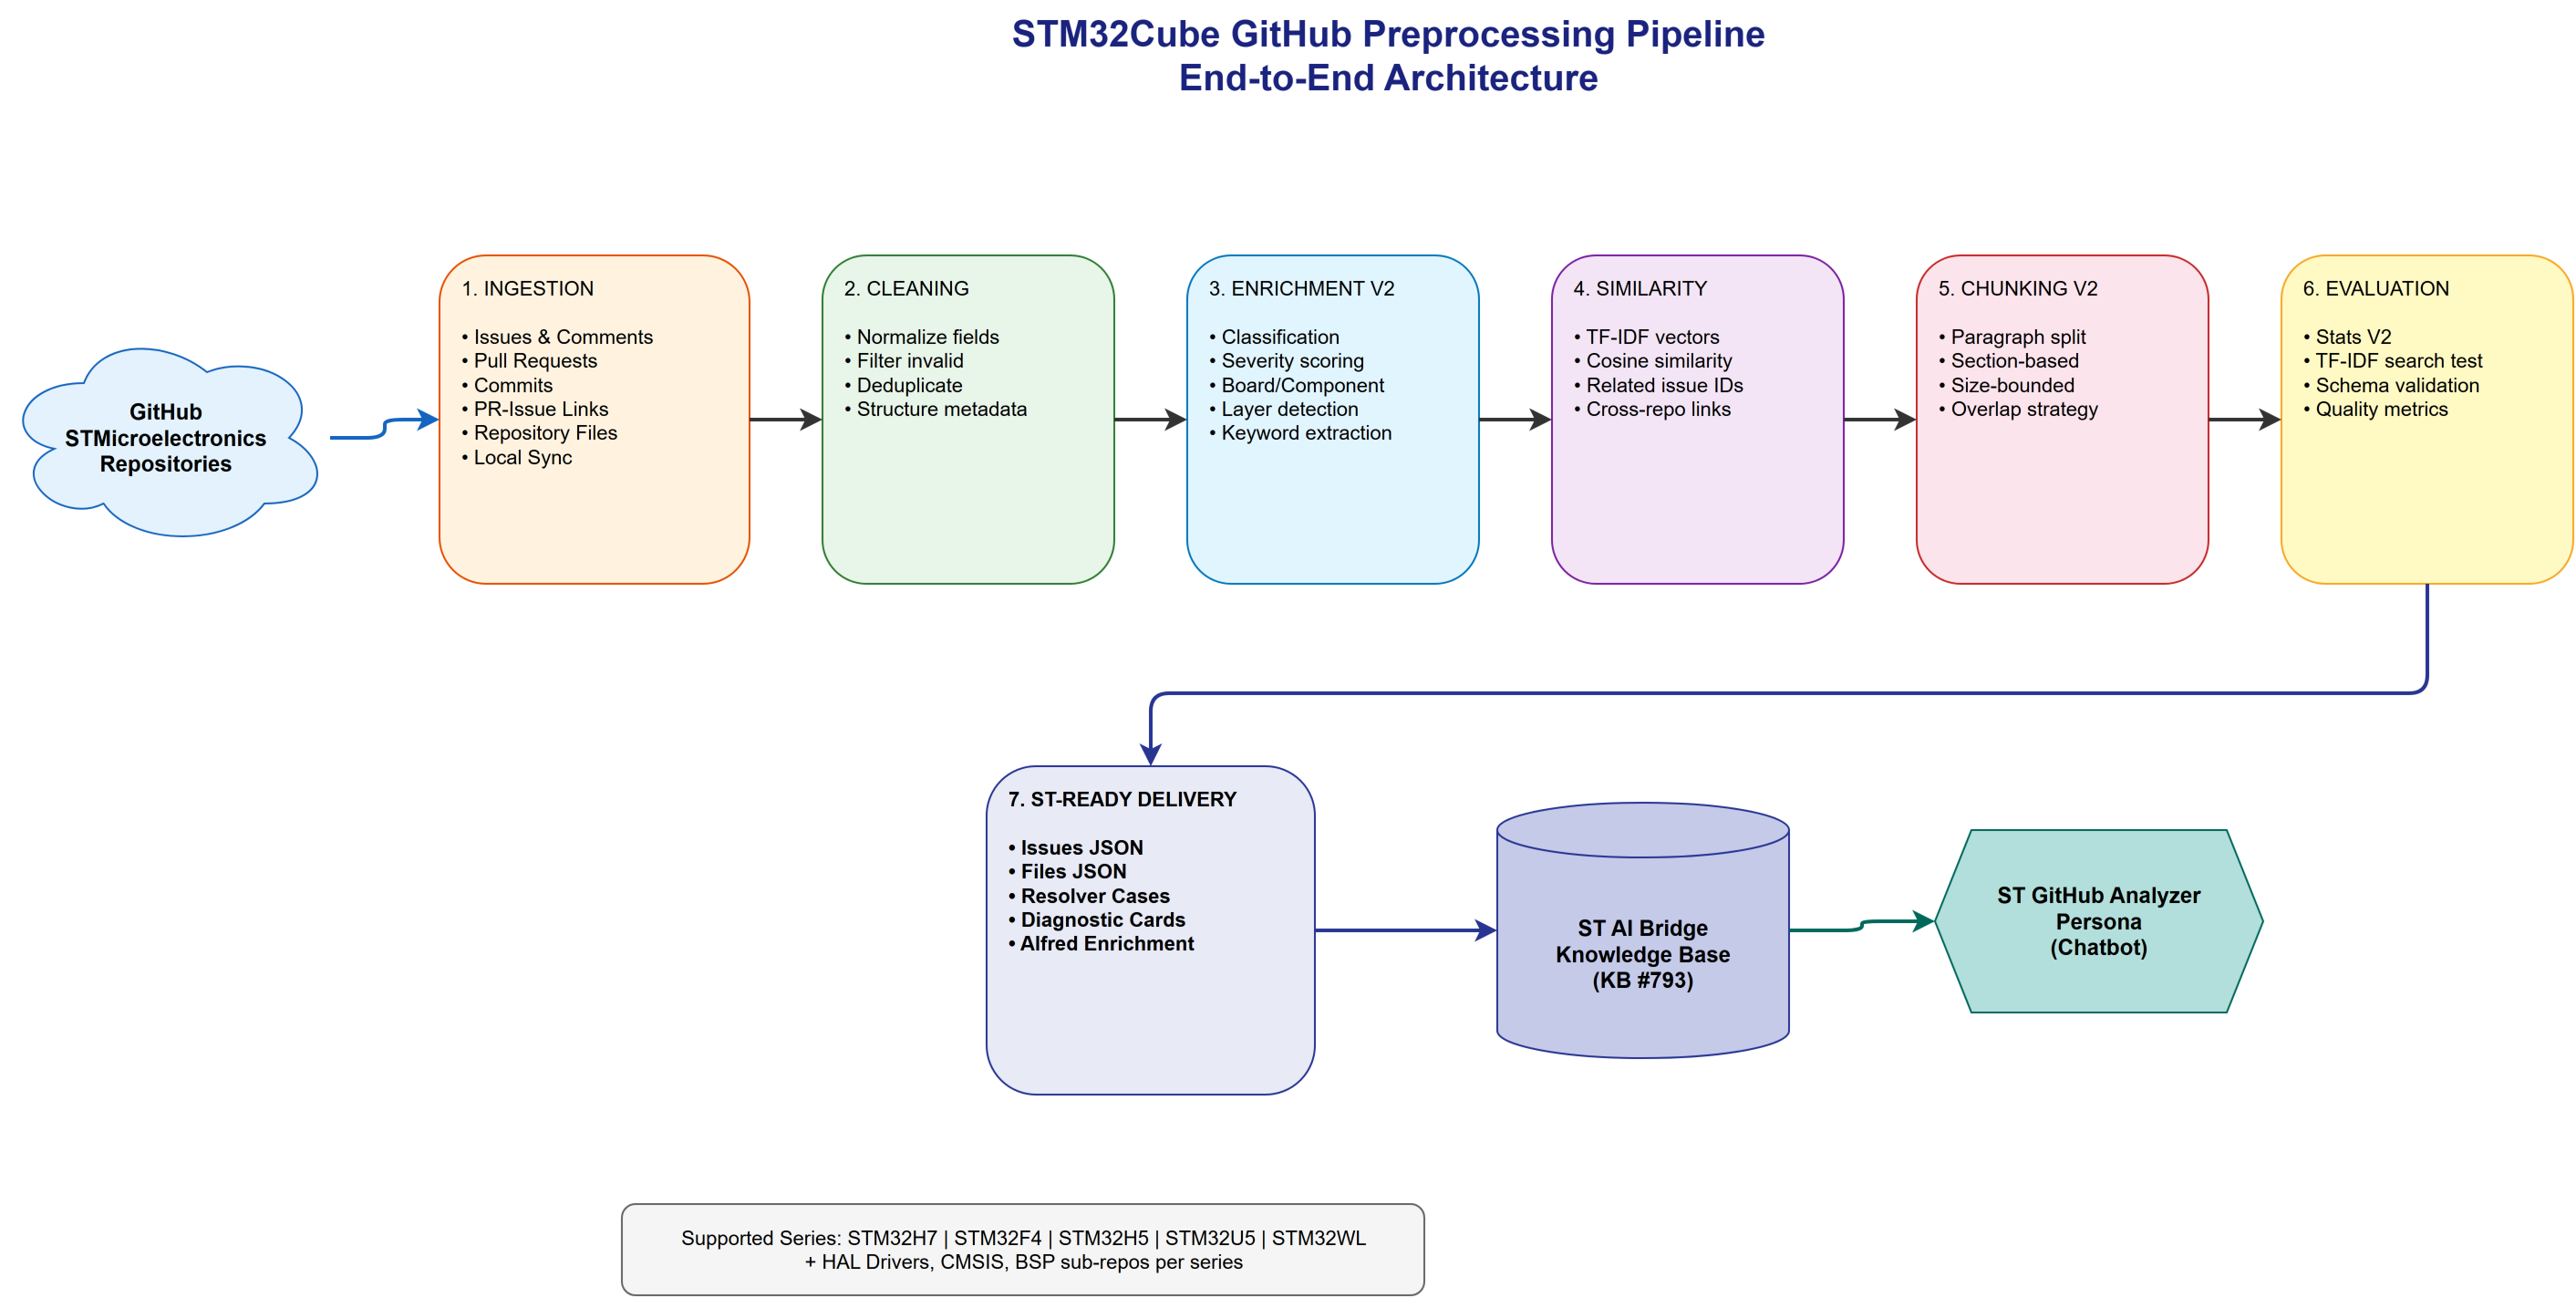
\includegraphics[width=0.95\textwidth]{01_pipeline_overview.png}
\caption{Vue d'ensemble du pipeline de preprocessing (7 stages)}
\label{fig:pipeline_overview}
\end{figure}

La Figure~\ref{fig:pipeline_arch_tikz} détaille les connexions entre stages, les fichiers intermédiaires produits à chaque étape, et le branchement de l'enrichissement Alfred Vision AI.

% Diagramme d'architecture pipeline - exporter depuis draw.io pour meilleure lisibilité
\begin{figure}[H]
\centering
\includegraphics[width=0.95\textwidth]{pipeline_architecture_detailed.png}
\caption{Architecture détaillée du pipeline : stages, fichiers intermédiaires et branchement Alfred (draw.io)}
\label{fig:pipeline_arch_tikz}
\end{figure}

\textit{Le diagramme montre le flux : GitHub (25 repos) $\to$ Ingestion (raw\_*) $\to$ Cleaning V1/V3 (clean\_*) $\to$ Enrichment (docs\_*) $\to$ Similarity (\_sim) $\to$ Validation $\to$ Delivery (st\_ready\_*) $\to$ Upload KB \#793 $\to$ ST ChatGPT. Alfred Vision intervient en parallèle pour décrire les images des issues et les figures PDF.}

\section{Flux Source-to-Answer}

La Figure~\ref{fig:data_flow} montre le parcours complet d'une donnée depuis GitHub jusqu'à la réponse au client final.

\begin{figure}[H]
\centering
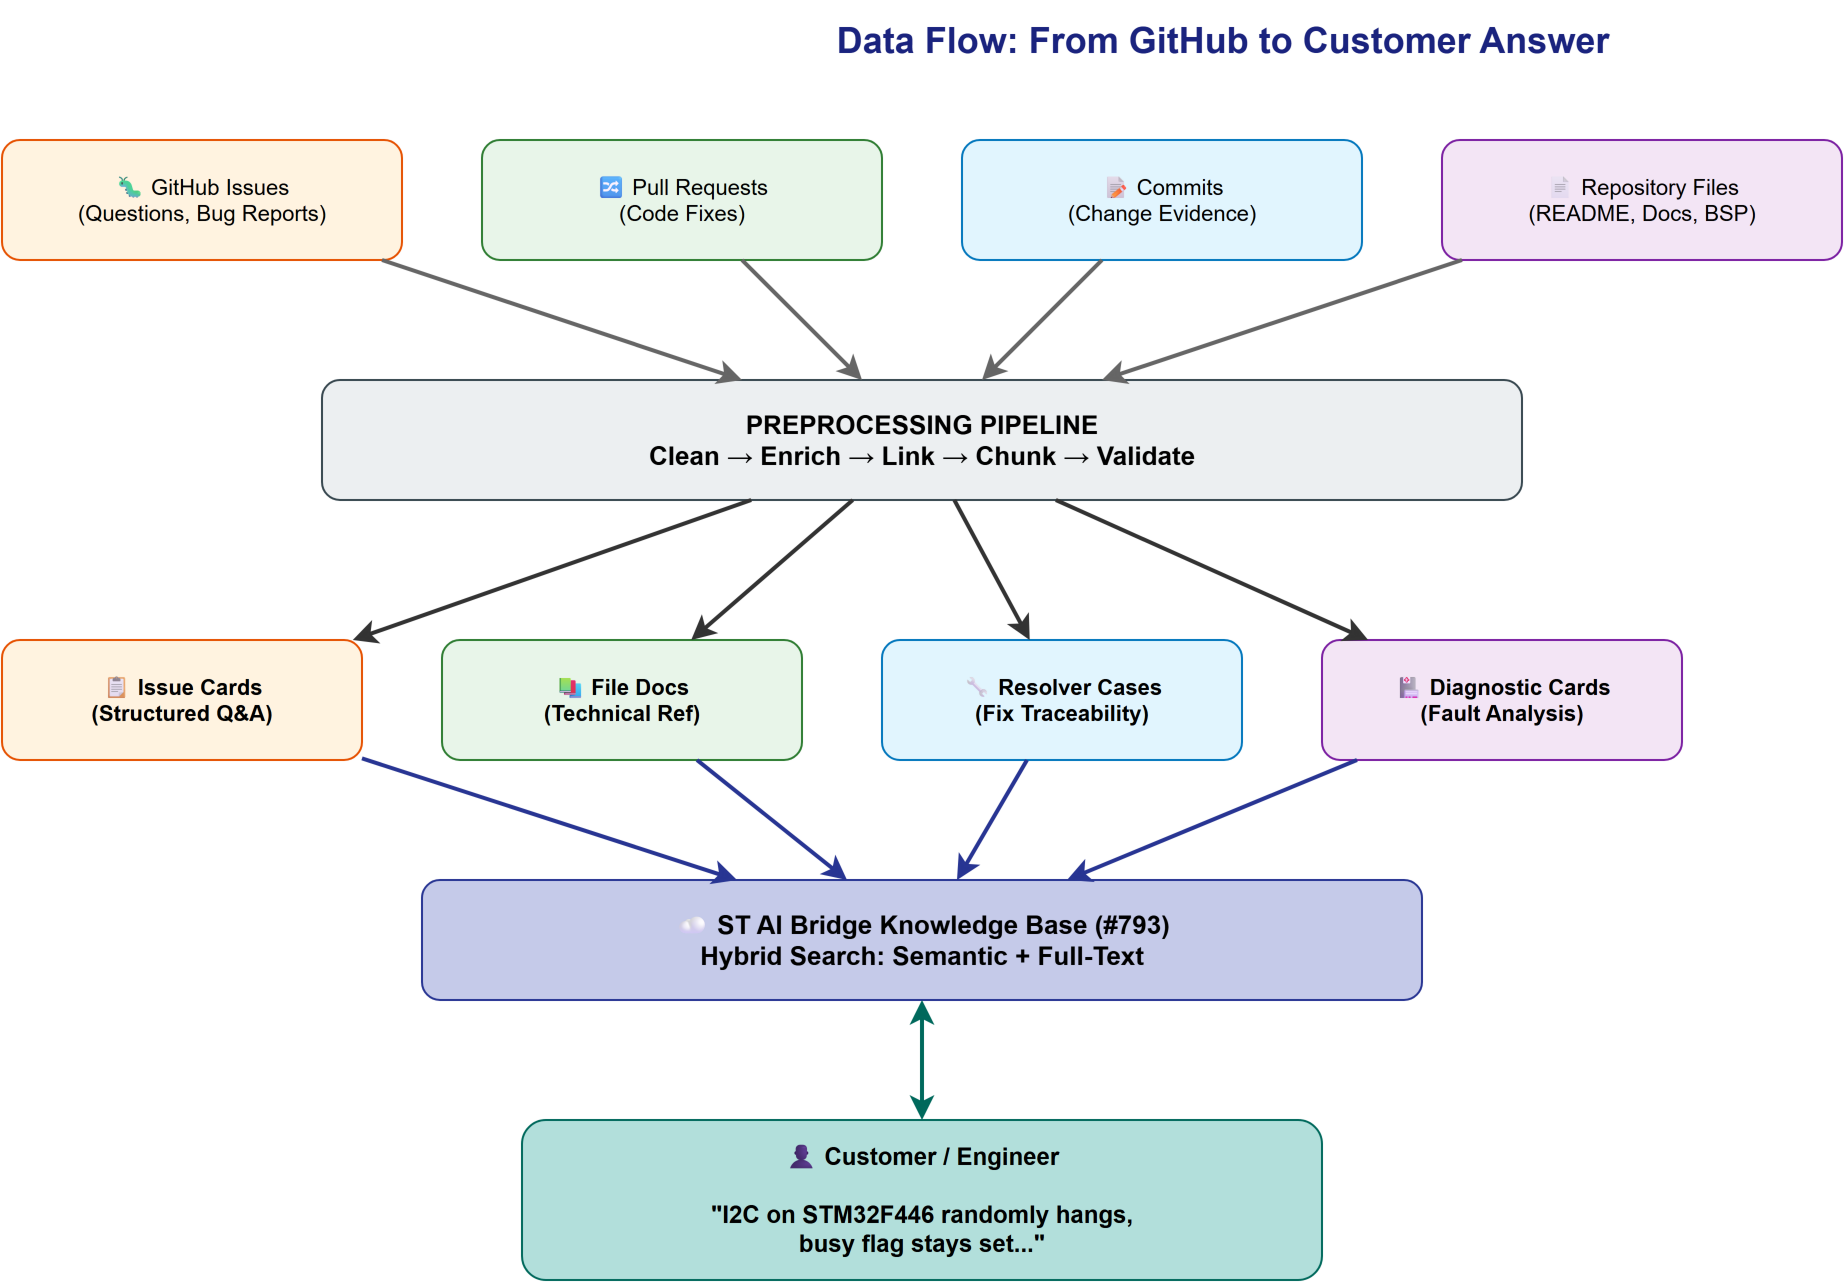
\includegraphics[width=0.95\textwidth]{03_data_flow_source_to_answer.png}
\caption{Flux de données end-to-end : de la source GitHub à la réponse utilisateur}
\label{fig:data_flow}
\end{figure}

\section{Architecture de Delivery et Upload KB}

\begin{figure}[H]
\centering
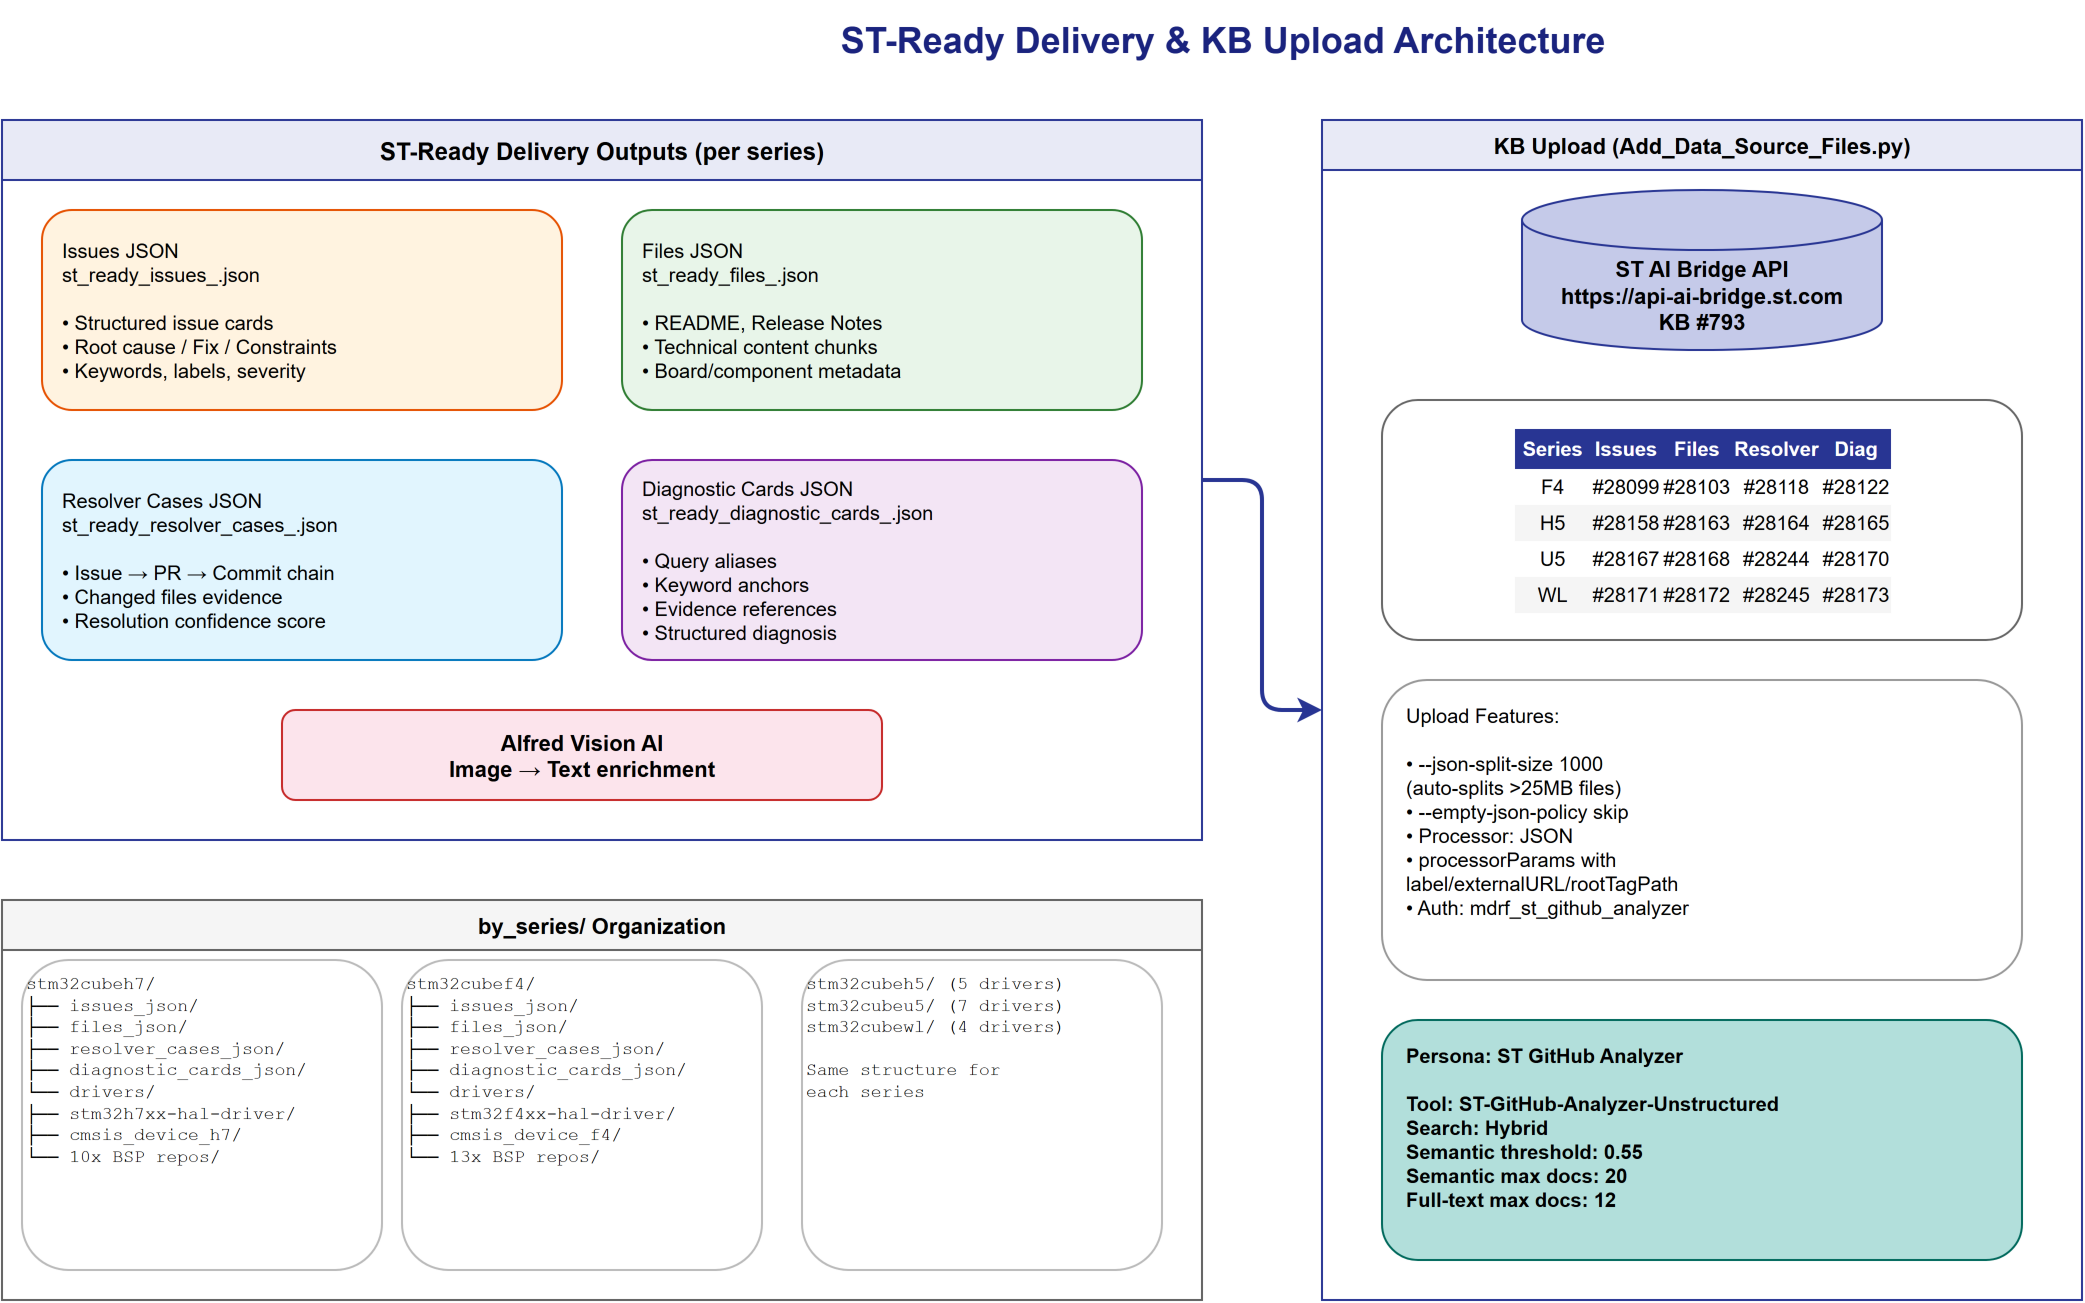
\includegraphics[width=0.9\textwidth]{02_delivery_kb_upload.png}
\caption{Architecture de livraison et upload vers la Knowledge Base \#793}
\label{fig:delivery_upload}
\end{figure}

%% ============================================================
\chapter{Implémentation}
%% ============================================================

\section{Ingestion (Stage 1)}

\subsection{Objectif}
Récupérer exhaustivement toutes les données des repositories GitHub configurés pour une série MCU donnée. La configuration est définie dans un fichier \texttt{config\_XX.json} qui liste les repos à ingérer.

\subsection{Mécanisme}
L'ingestion s'appuie sur 5 scripts spécialisés :
\begin{itemize}
  \item \texttt{fetch\_issues.py} : récupère toutes les issues (ouvertes + fermées) avec leurs commentaires, via l'API GitHub REST avec pagination automatique (100 items/page)
  \item \texttt{fetch\_prs.py} : récupère les Pull Requests et leurs reviews
  \item \texttt{fetch\_commits.py} : récupère l'historique des commits pour le linking Issue$\to$PR$\to$Commit
  \item \texttt{fetch\_issue\_pr\_commit\_links.py} : construit les chaînes de traçabilité croisées
  \item \texttt{repo\_sync\_service.py} : clone/met à jour les repos localement pour l'extraction de fichiers
  \item \texttt{fetch\_files.py} : parcourt l'arborescence des repos clonés et extrait le contenu des fichiers pertinents (README, Release Notes, sources, PDFs)
\end{itemize}

\textbf{Gestion du rate-limiting} : l'API GitHub autorise 5\,000 requêtes/heure avec un token d'authentification. Le pipeline implémente un sleep adaptatif (0,2s entre les issues, 0,1s entre les commentaires) et un retry exponentiel en cas d'erreur 403/429.

\subsection{Exemple de Sortie --- Issue Brute}

\begin{lstlisting}[language=json, caption={Extrait de raw\_issues\_stm32cubeh7.json (issue brute)}]
{
  "number": 42,
  "title": "HAL_SPI_TransmitReceive_DMA fails on STM32H743",
  "state": "closed",
  "labels": ["bug"],
  "body": "When using HAL_SPI_TransmitReceive_DMA with...",
  "comments": [
    {"user": "dev123", "body": "Same issue on NUCLEO-H743ZI..."},
    {"user": "st-support", "body": "Fixed in v1.11.0..."}
  ],
  "created_at": "2023-06-15T10:30:00Z",
  "closed_at": "2023-08-20T14:00:00Z"
}
\end{lstlisting}

% Diagramme d'ingestion - exporter depuis draw.io
\begin{figure}[H]
\centering
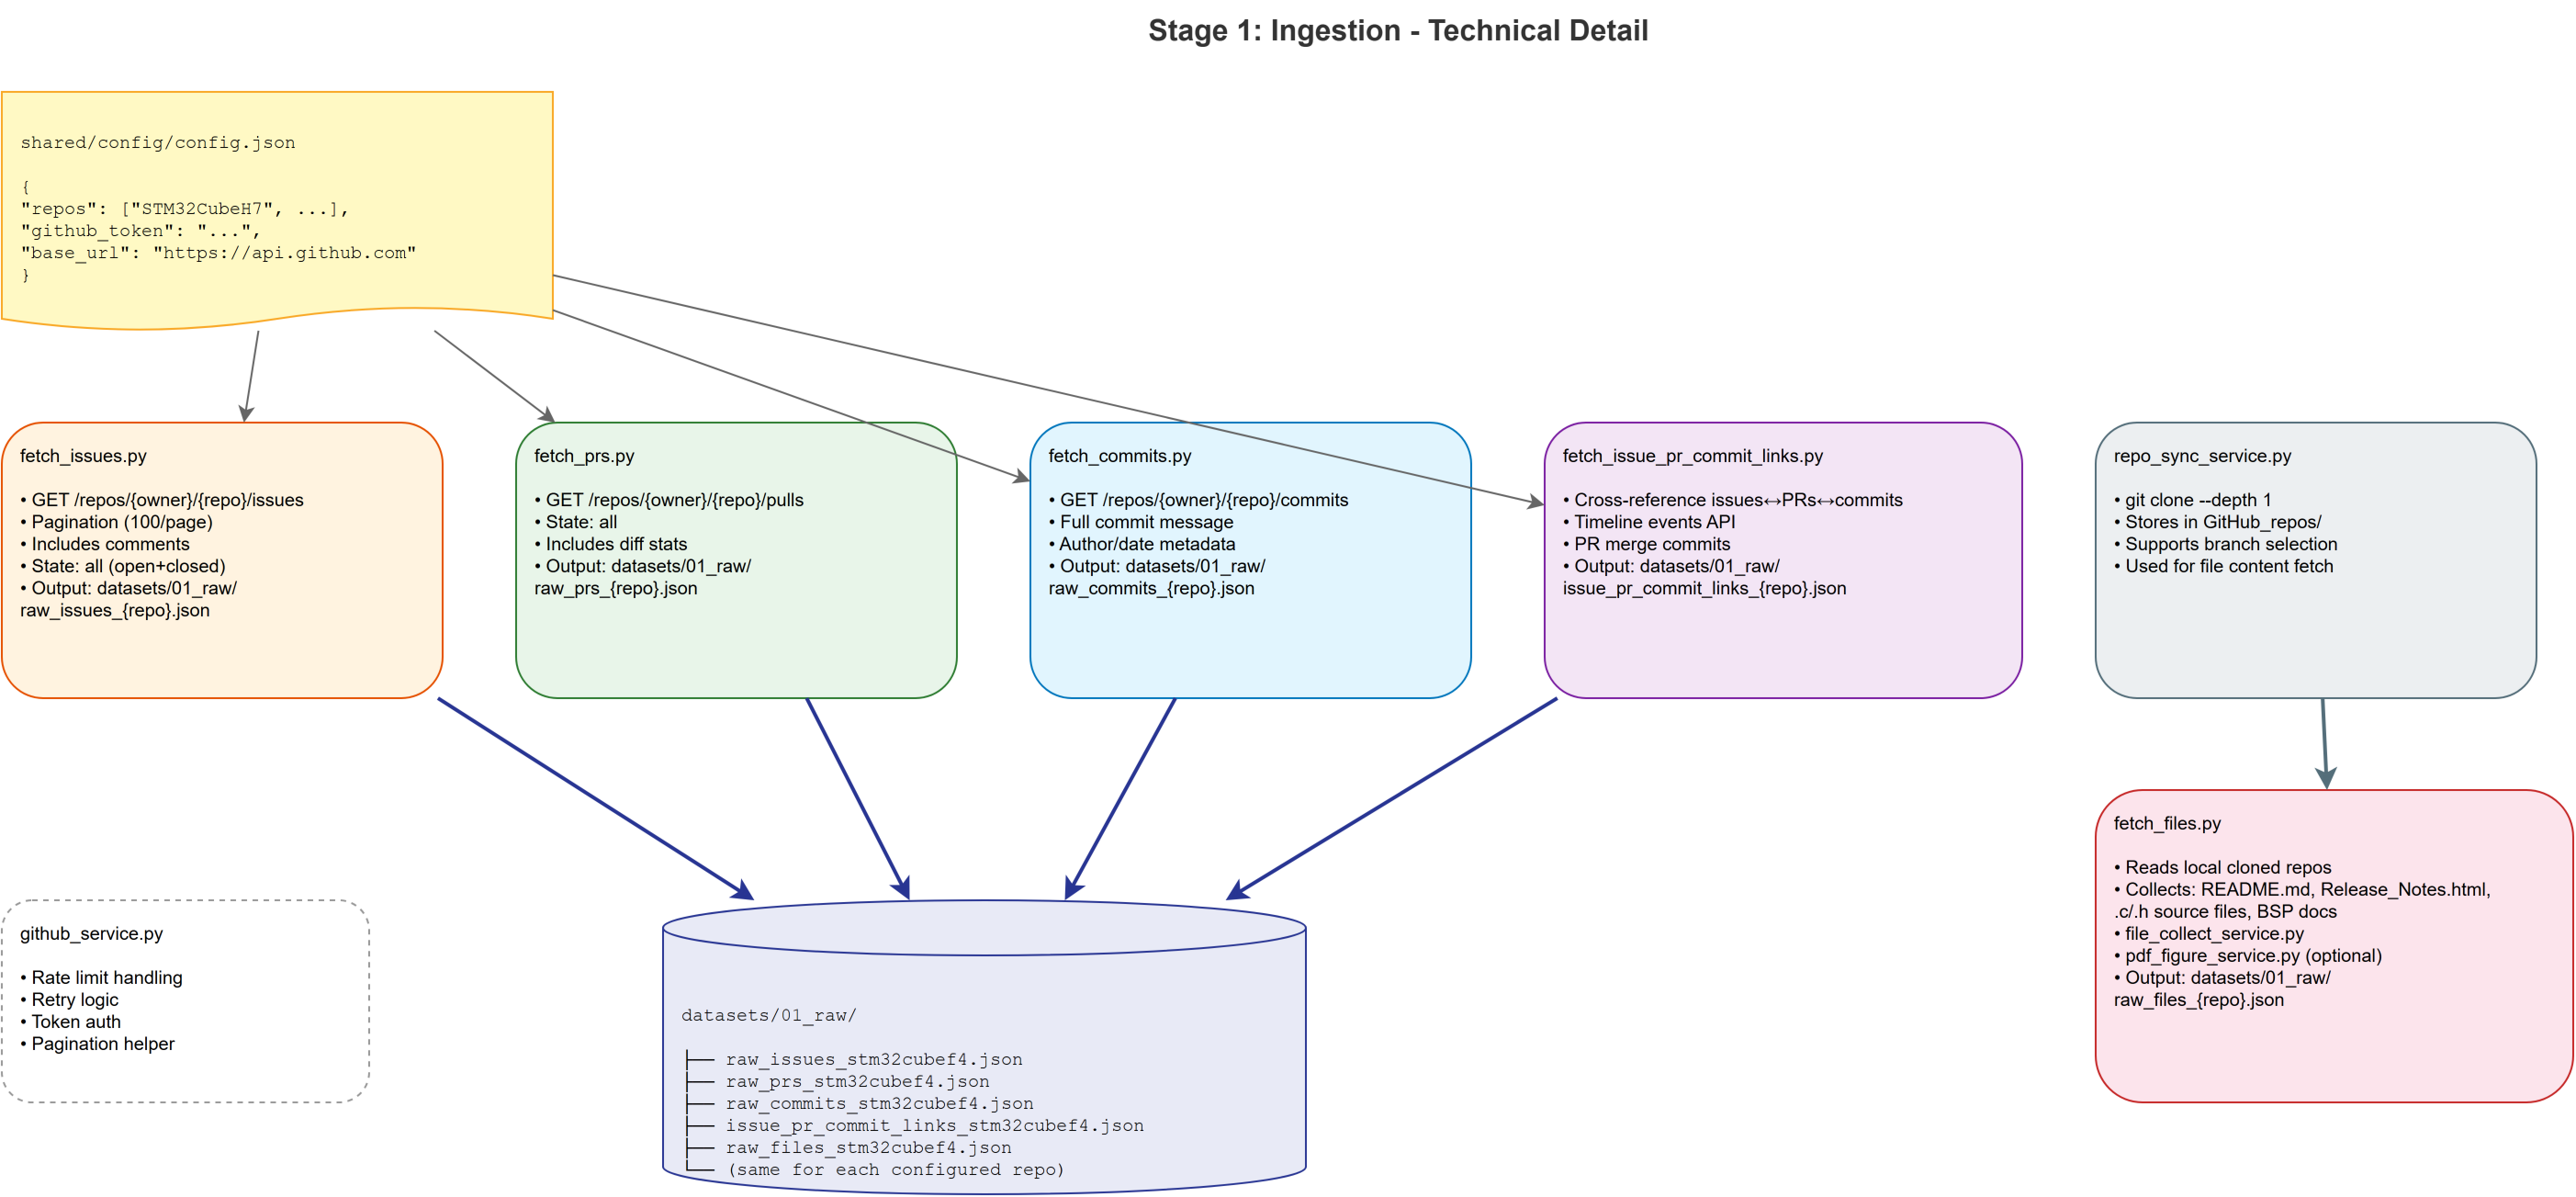
\includegraphics[width=0.9\textwidth]{01_ingestion_detail.png}
\caption{Détail de l'étape d'ingestion : scripts et sorties (draw.io)}
\label{fig:ingestion_detail}
\end{figure}

\section{Nettoyage (Stage 2)}

Le nettoyage prépare les données brutes pour l'enrichissement en éliminant le bruit textuel :

\subsection{Nettoyage des Issues}
\begin{itemize}
  \item Normalisation du texte (retours chariot, backticks, espaces)
  \item Extraction des images en markers \texttt{[IMAGE ATTACHED]} avec collecte des URLs
  \item Structuration : assemblage Title + Body + Comments en un seul champ \texttt{clean\_text}
  \item Conservation des métadonnées brutes (labels, dates, état)
\end{itemize}

\subsection{Exemple JSON --- Issue Après Nettoyage}

\begin{lstlisting}[language=json, caption={Extrait de clean\_issues\_stm32cubeh7.json (issue nettoyée)}]
{
  "number": 42,
  "title": "HAL_SPI_TransmitReceive_DMA fails on STM32H743",
  "state": "closed",
  "labels": ["bug"],
  "clean_text": "HAL_SPI_TransmitReceive_DMA fails on STM32H743. When using HAL_SPI_TransmitReceive_DMA with circular mode and cache enabled, a hard fault occurs after the second transfer. [IMAGE ATTACHED: screenshot_debugger.png] Workaround: disable D-cache before SPI init. Same issue on NUCLEO-H743ZI with CubeH7 v1.10.0. Fixed in v1.11.0 by adding cache maintenance in HAL_SPI_TxRxCpltCallback.",
  "images_count": 1,
  "image_urls": ["https://user-images.githubusercontent.com/xxx/screenshot_debugger.png"],
  "created_at": "2023-06-15T10:30:00Z",
  "closed_at": "2023-08-20T14:00:00Z"
}
\end{lstlisting}

\textbf{Transformation clé} : le champ \texttt{clean\_text} fusionne le titre, le body et tous les commentaires de l'issue en un seul texte contigu, prêt pour l'enrichissement NLP. Les images sont remplacées par des markers textuels avec leurs URLs collectées séparément pour l'enrichissement Alfred Vision.

\subsection{Nettoyage des Fichiers}
\begin{itemize}
  \item Lecture du contenu (UTF-8, fallback Latin-1)
  \item Extraction du texte des PDFs (pypdf + rendu pages + détection figures OpenCV)
  \item Construction de l'URL GitHub pour chaque fichier
  \item Filtrage : seuls les fichiers pertinents sont retenus (README, Release Notes, source technique, documentation PDF)
\end{itemize}

\subsection{Exemple JSON --- Fichier Après Nettoyage}

\begin{lstlisting}[language=json, caption={Extrait de clean\_files\_stm32h7xx-hal-driver.json}]
{
  "path": "Src/stm32h7xx_hal_spi.c",
  "repo": "stm32h7xx-hal-driver",
  "file_type": "source_code",
  "url": "https://github.com/STMicroelectronics/stm32h7xx-hal-driver/blob/master/Src/stm32h7xx_hal_spi.c",
  "original_size": 89247,
  "clean_size": 80322,
  "is_valid": true,
  "clean_text": "HAL_StatusTypeDef HAL_SPI_Init(SPI_HandleTypeDef *hspi) { ... } HAL_StatusTypeDef HAL_SPI_TransmitReceive_DMA(...) { ... }"
}
\end{lstlisting}

\textbf{Transformation clé} : le bloc de licence en-tête (copyright STMicroelectronics, 20--40 lignes) est supprimé par \texttt{strip\_license()}, réduisant le bruit de $\sim$10\%. Le champ \texttt{is\_valid} passe à \texttt{false} si le texte nettoyé fait moins de 100 caractères.

\textbf{Note importante} : Le nettoyage ne fait \textbf{aucune classification} (pas de détection de layer, board, component). Cette tâche est réalisée à l'étape suivante (Enrichissement).

\section{Nettoyage V3 --- Nettoyage Intelligent par Type (Stage 2b)}

Le nettoyage V1/V2 appliquait une stratégie uniforme à tous les fichiers. Or les sources ingérées sont hétérogènes : Release Notes en HTML, README en Markdown avec badges, fichiers source C avec licences volumineuses, et headers CMSIS de plus d'1~Mo. La version 3 introduit un \textbf{nettoyage par type} qui adapte la stratégie au contenu réel de chaque fichier.

\subsection{Stratégies de Nettoyage par Type}

Le script \texttt{clean\_files\_v3.py} route chaque fichier vers une stratégie spécialisée :

\begin{longtable}{p{3.5cm}p{3.5cm}p{6cm}}
\toprule
\textbf{Type détecté} & \textbf{Stratégie} & \textbf{Transformations appliquées} \\
\midrule
Release Notes & \texttt{strip\_html()} & Suppression balises HTML, conservation texte pur, normalisation espaces \\
README / .md & \texttt{clean\_markdown()} & Suppression badges CI, liens images, normalisation titres \\
Source code (.c/.h) & \texttt{clean\_source\_code()} & Suppression bloc licence (copyright), conservation code technique \\
CMSIS device header & \texttt{filter\_cmsis\_device\_header()} & Filtrage intelligent (voir ci-dessous) \\
Autres & Inchangé & Aucune transformation \\
\bottomrule
\end{longtable}

La Figure~\ref{fig:cleaning_v3_tree} représente l'arbre de décision du routage V3, avec les taux de réduction mesurés pour chaque stratégie.

% Arbre de décision V3 - exporter depuis draw.io
\begin{figure}[H]
\centering
\includegraphics[width=0.9\textwidth]{cleaning_v3_decision_tree.png}
\caption{Arbre de décision du nettoyage V3 : routage par type de fichier avec taux de réduction (draw.io)}
\label{fig:cleaning_v3_tree}
\end{figure}

\textit{L'arbre de décision route chaque fichier via \texttt{detect\_file\_type()} vers la stratégie adaptée : release\_notes $\to$ strip\_html() ($-33\%$), readme $\to$ clean\_md() ($-15\%$), source $\to$ strip\_license() ($-10\%$), cmsis $>$100~Ko $\to$ filter\_cmsis() ($-96\%$), other $\to$ passthrough.}

\subsection{Filtrage CMSIS Device Headers}

Les fichiers de type \texttt{stm32*xx.h} (CMSIS device) sont les plus volumineux du corpus (1--1.7~Mo). Ils contiennent principalement des définitions de registres bit-à-bit inutiles pour le RAG. Le filtre V3 ne conserve que les sections à valeur diagnostique :

\begin{enumerate}
  \item \textbf{Énumération IRQ} : liste des vecteurs d'interruption (\texttt{typedef enum IRQn})
  \item \textbf{Adresses de base} : adresses mémoire des périphériques (\texttt{\#define PERIPH\_BASE})
  \item \textbf{Structures TypeDef} : définitions de registres par périphérique (\texttt{typedef struct \{...\}})
\end{enumerate}

\textbf{Seuil d'activation} : le filtre ne s'applique qu'aux fichiers dépassant 100~Ko (les petits headers sont conservés intégralement).

\subsection{Résultat du Filtrage --- Exemple JSON}

Voici un extrait du fichier \texttt{clean\_files\_cmsis\_device\_h7\_v3.json} montrant un header CMSIS après filtrage V3 :

\begin{lstlisting}[language=json, caption={Header CMSIS après filtrage V3 (extrait)}]
{
  "path": "Include/stm32h743xx.h",
  "repo": "cmsis_device_h7",
  "file_type": "cmsis_device_header",
  "original_size": 1458301,
  "clean_size": 52140,
  "reduction_pct": 96.4,
  "is_valid": true,
  "clean_text": "typedef enum { NonMaskableInt_IRQn = -14, ... } IRQn_Type; #define PERIPH_BASE 0x40000000UL ... typedef struct { __IO uint32_t CR1; __IO uint32_t CR2; ... } SPI_TypeDef;"
}
\end{lstlisting}

Le fichier passe de 1\,458\,301 caractères à 52\,140 ($-96,4\%$), ne conservant que les IRQ, adresses de base et TypeDef.

\subsection{Résultats du Nettoyage V3}

\begin{longtable}{p{5cm}ccc}
\toprule
\textbf{Fichier} & \textbf{Taille V2} & \textbf{Taille V3} & \textbf{Réduction} \\
\midrule
\texttt{stm32h503xx.h} & 1\,074\,499 & 36\,499 & $-96.6\%$ \\
\texttt{stm32h562xx.h} & 1\,722\,072 & 65\,470 & $-96.2\%$ \\
\texttt{stm32h743xx.h} & 1\,458\,301 & 52\,140 & $-96.4\%$ \\
Release Notes (moy.) & 45\,200 & 30\,300 & $-33.0\%$ \\
Sources avec licence & 12\,800 & 11\,500 & $-10.2\%$ \\
\bottomrule
\end{longtable}

\textbf{Impact global} : Sur les 47 repos (5 séries MCU), le volume total des fichiers nettoyés est réduit de \textbf{38\%} en moyenne, ce qui améliore directement la densité d'information des chunks et la pertinence du retrieval.

\subsection{Compatibilité et Non-Régression}

Le V3 n'écrase jamais les sorties V1/V2 :
\begin{itemize}
  \item Fichiers d'entrée : \texttt{clean\_files\_<repo>.json} (V1) ou \texttt{clean\_files\_<repo>\_v3.json} (V3)
  \item Les étapes aval (enrichissement, delivery) acceptent un flag \texttt{--v3} pour router automatiquement vers les fichiers V3
  \item Les datasources V3 sont uploadées vers des IDs séparés (29041--29045)
\end{itemize}

\section{Enrichissement V2 (Stage 3)}

\subsection{Heuristiques de Classification}

Le module \texttt{stm32cube\_preprocessing\_heuristics.py} applique des règles basées sur :
\begin{itemize}
  \item \textbf{Regex patterns} : détection de séries MCU, composants, boards
  \item \textbf{Analyse des labels} : mapping label→layer (bug→bug\_report, etc.)
  \item \textbf{Scoring pondéré} : longueur du body, présence de code, de logs d'erreur
\end{itemize}

\subsection{Exemple de Classification}

\begin{lstlisting}[language=json]
{
  "issue_number": 42,
  "title": "HAL_SPI_TransmitReceive DMA fails on STM32F446",
  "layer": "HAL",
  "component": "SPI", 
  "board": "NUCLEO-F446RE",
  "issue_kind": "bug_report",
  "severity": "high",
  "evidence_strength": "high"
}
\end{lstlisting}

\section{Similarité (Stage 4)}

\subsection{Algorithme}
\begin{enumerate}
  \item Construction de la matrice TF-IDF sur le corpus (titre + body + commentaires) :
  \begin{equation}
    \text{tf-idf}(t, d) = \text{tf}(t,d) \times \log\frac{N}{|\{d' \mid t \in d'\}|}
  \end{equation}
  \item Calcul de la similarité cosinus paire-à-paire :
  \begin{equation}
    \text{sim}(d_i, d_j) = \frac{\vec{v}_i \cdot \vec{v}_j}{\|\vec{v}_i\| \times \|\vec{v}_j\|}
  \end{equation}
  \item Sélection des $k$ plus proches voisins avec seuil $\theta = 0.3$ :
  \begin{equation}
    \text{related}(d_i) = \{d_j \mid \text{sim}(d_i, d_j) \geq \theta,\ j \neq i\}
  \end{equation}
\end{enumerate}

\subsection{Exemple JSON --- Issue avec Liens de Similarité}

\begin{lstlisting}[language=json, caption={Extrait de docs\_issues\_stm32cubeh7\_v2\_sim.json (avec voisins)}]
{
  "issue_number": 42,
  "title": "HAL_SPI_TransmitReceive_DMA fails on STM32H743",
  "similar_issues": [
    {"issue_number": 78, "similarity": 0.72, "title": "SPI DMA circular mode crash H750"},
    {"issue_number": 156, "similarity": 0.45, "title": "DMA cache coherency issue H743"},
    {"issue_number": 203, "similarity": 0.38, "title": "Hard fault after second SPI transfer"}
  ],
  "related_count": 3
}
\end{lstlisting}

\textbf{Paramètres} : le seuil $\theta = 0.3$ élimine les liens trop faibles (bruit). Sur H7, seulement 22\% des issues ont au moins un voisin au-dessus de ce seuil, ce qui reflète la diversité des problèmes (chaque issue traite un bug unique). Le nombre $k$ de voisins n'est pas borné --- toutes les paires dépassant $\theta$ sont conservées.

\begin{figure}[H]
\centering
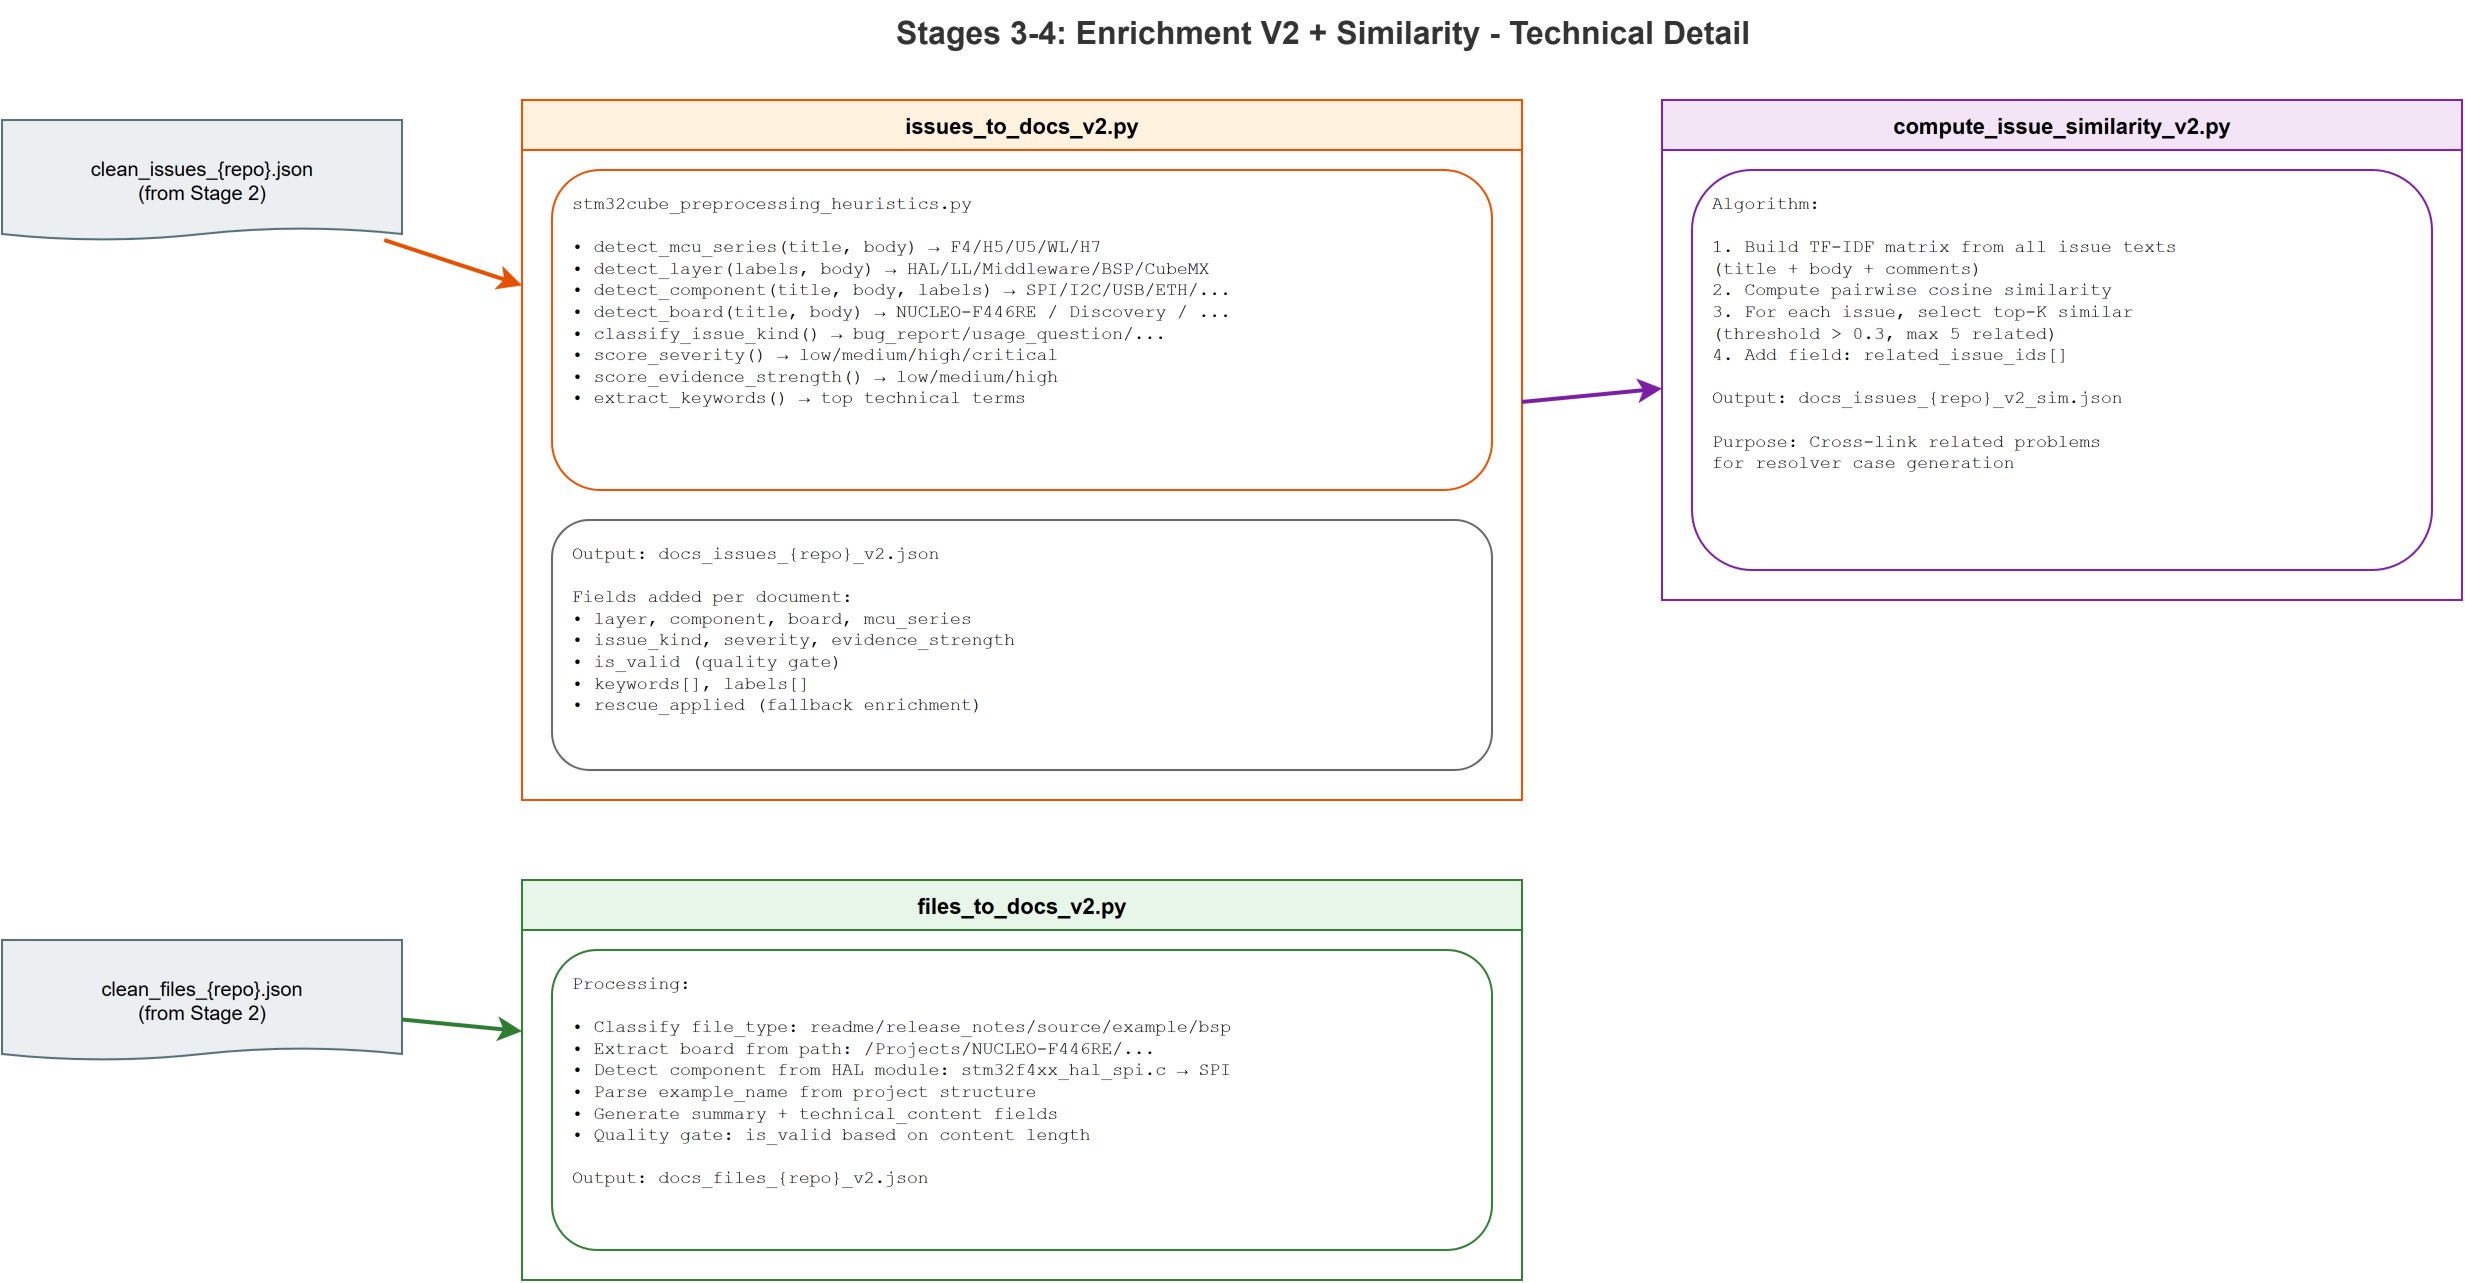
\includegraphics[width=0.85\textwidth]{02_enrichment_similarity_detail.png}
\caption{Détail du processus d'enrichissement et de calcul de similarité}
\label{fig:enrichment_similarity}
\end{figure}

\section{Chunking V2 (Stage 5 --- Optionnel)}

\textbf{Note importante} : le chunking est réalisé localement à des fins de \textbf{test et validation} uniquement. En production, la plateforme ST ChatGPT gère elle-même le découpage des documents lors de l'indexation (paramètre \texttt{json-split-size: 1000}). Le chunking local nous permet de :
\begin{itemize}
  \item Vérifier la taille et la qualité des segments avant upload
  \item Tester la recherche TF-IDF en local (évaluation préliminaire)
  \item Comparer les stratégies de découpage sans impacter la KB en production
\end{itemize}

Stratégie de découpage local :
\begin{itemize}
  \item Issues : chunks par paragraphe, max 512 tokens, overlap 50 tokens
  \item Files : chunks par section (README headers, fonctions C)
\end{itemize}

Le flag \texttt{--skip-chunking} dans le workflow permet de sauter cette étape pour les runs de production, car la plateforme gère le chunking automatiquement à l'upload.

\section{Delivery (Stage 7)}

\subsection{Resolver Cases}
Générés à partir d'issues fermées avec PRs liées :
\begin{enumerate}
  \item Identification de la chaîne Issue $\to$ PR $\to$ Commits via \texttt{fetch\_issue\_pr\_commit\_links.py}
  \item Évaluation du \texttt{resolution\_status} :
  \begin{itemize}
    \item \texttt{merged\_fix} : PR mergée avec fichiers modifiés identifiés (confiance haute)
    \item \texttt{candidate\_fix} : PR liée mais non mergée ou lien faible (confiance moyenne)
    \item \texttt{reference\_only} : issue résolue sans PR formelle (information contextuelle)
  \end{itemize}
  \item Construction du texte structuré : Problème $\to$ Signal $\to$ Évaluation $\to$ Preuves
\end{enumerate}

\subsection{Exemple JSON --- Resolver Case}

\begin{lstlisting}[language=json, caption={Extrait de st\_ready\_resolver\_stm32cubeh7.json}]
{
  "issue_number": 42,
  "repo": "stm32cubeh7",
  "label": "SPI DMA TransmitReceive fails on STM32H743 in circular mode",
  "resolution_status": "merged_fix",
  "link_confidence": "high",
  "primary_pr_number": 87,
  "primary_changed_file": "Src/stm32h7xx_hal_spi.c",
  "resolver_card_text": "PROBLEM: HAL_SPI_TransmitReceive_DMA causes hard fault after second transfer in circular mode. SIGNAL: D-cache stale read on DMA buffer. EVALUATION: Cache maintenance missing in TxRxCpltCallback. FIX: Added SCB_InvalidateDCache_by_Addr() call in HAL_SPI_TxRxCpltCallback. PROOF: PR #87 merged 2023-08-15, verified on NUCLEO-H743ZI.",
  "impacted_modules": ["SPI", "DMA"],
  "impacted_boards": ["NUCLEO-H743ZI"]
}
\end{lstlisting}

\textbf{Valeur ajoutée} : contrairement aux issues brutes, le Resolver Case fournit la \textbf{chaîne de preuves complète} (issue $\to$ PR \#87 $\to$ fichier modifié \texttt{stm32h7xx\_hal\_spi.c}) en un seul document. L'ingénieur peut vérifier le fix exact en suivant les liens.

\subsection{Diagnostic Cards}
Cartes de diagnostic structurées pour les problèmes récurrents :
\begin{enumerate}
  \item Sélection des issues à haute valeur diagnostique (issues fermées avec root cause identifié, \texttt{evidence\_strength} $\geq$ \texttt{medium})
  \item Génération : Symptôme $\to$ Cause Racine $\to$ Résolution $\to$ Validation
  \item Ajout de \textbf{query aliases} (reformulations multiples du problème) pour améliorer le recall de la recherche RAG
\end{enumerate}

\subsection{Exemple JSON --- Diagnostic Card}

\begin{lstlisting}[language=json, caption={Extrait de st\_ready\_diagnostic\_stm32cubeh7.json}]
{
  "diagnostic_id": "DIAG-H7-042",
  "repo": "stm32cubeh7",
  "issue_number": 42,
  "symptom": "Hard fault occurs after second SPI DMA transfer in circular mode on STM32H743",
  "root_cause": "D-cache not invalidated before DMA reception. CPU reads stale data from cache instead of DMA-updated SRAM.",
  "resolution": "Call SCB_InvalidateDCache_by_Addr() before reading SPI RX buffer, or place DMA buffers in non-cacheable SRAM region (MPU configuration).",
  "affected_versions": ["CubeH7 v1.9.0", "CubeH7 v1.10.0"],
  "fixed_version": "CubeH7 v1.11.0",
  "query_aliases": [
    "SPI DMA hard fault STM32H7",
    "cache coherency SPI circular mode",
    "HAL_SPI_TransmitReceive_DMA crash",
    "D-cache DMA corruption H743"
  ],
  "evidence_strength": "high",
  "impacted_boards": ["NUCLEO-H743ZI", "STM32H743I-EVAL"]
}
\end{lstlisting}

\textbf{Structure clé} : les \texttt{query\_aliases} sont le mécanisme principal d'amélioration du recall. Lorsqu'un utilisateur pose la question ``mon SPI crash après le 2e transfert DMA'', la recherche hybride retrouve cette Diagnostic Card grâce aux alias qui couvrent différentes formulations du même problème. C'est cette structure qui explique le saut de QI de 61 à 94.

\begin{figure}[H]
\centering
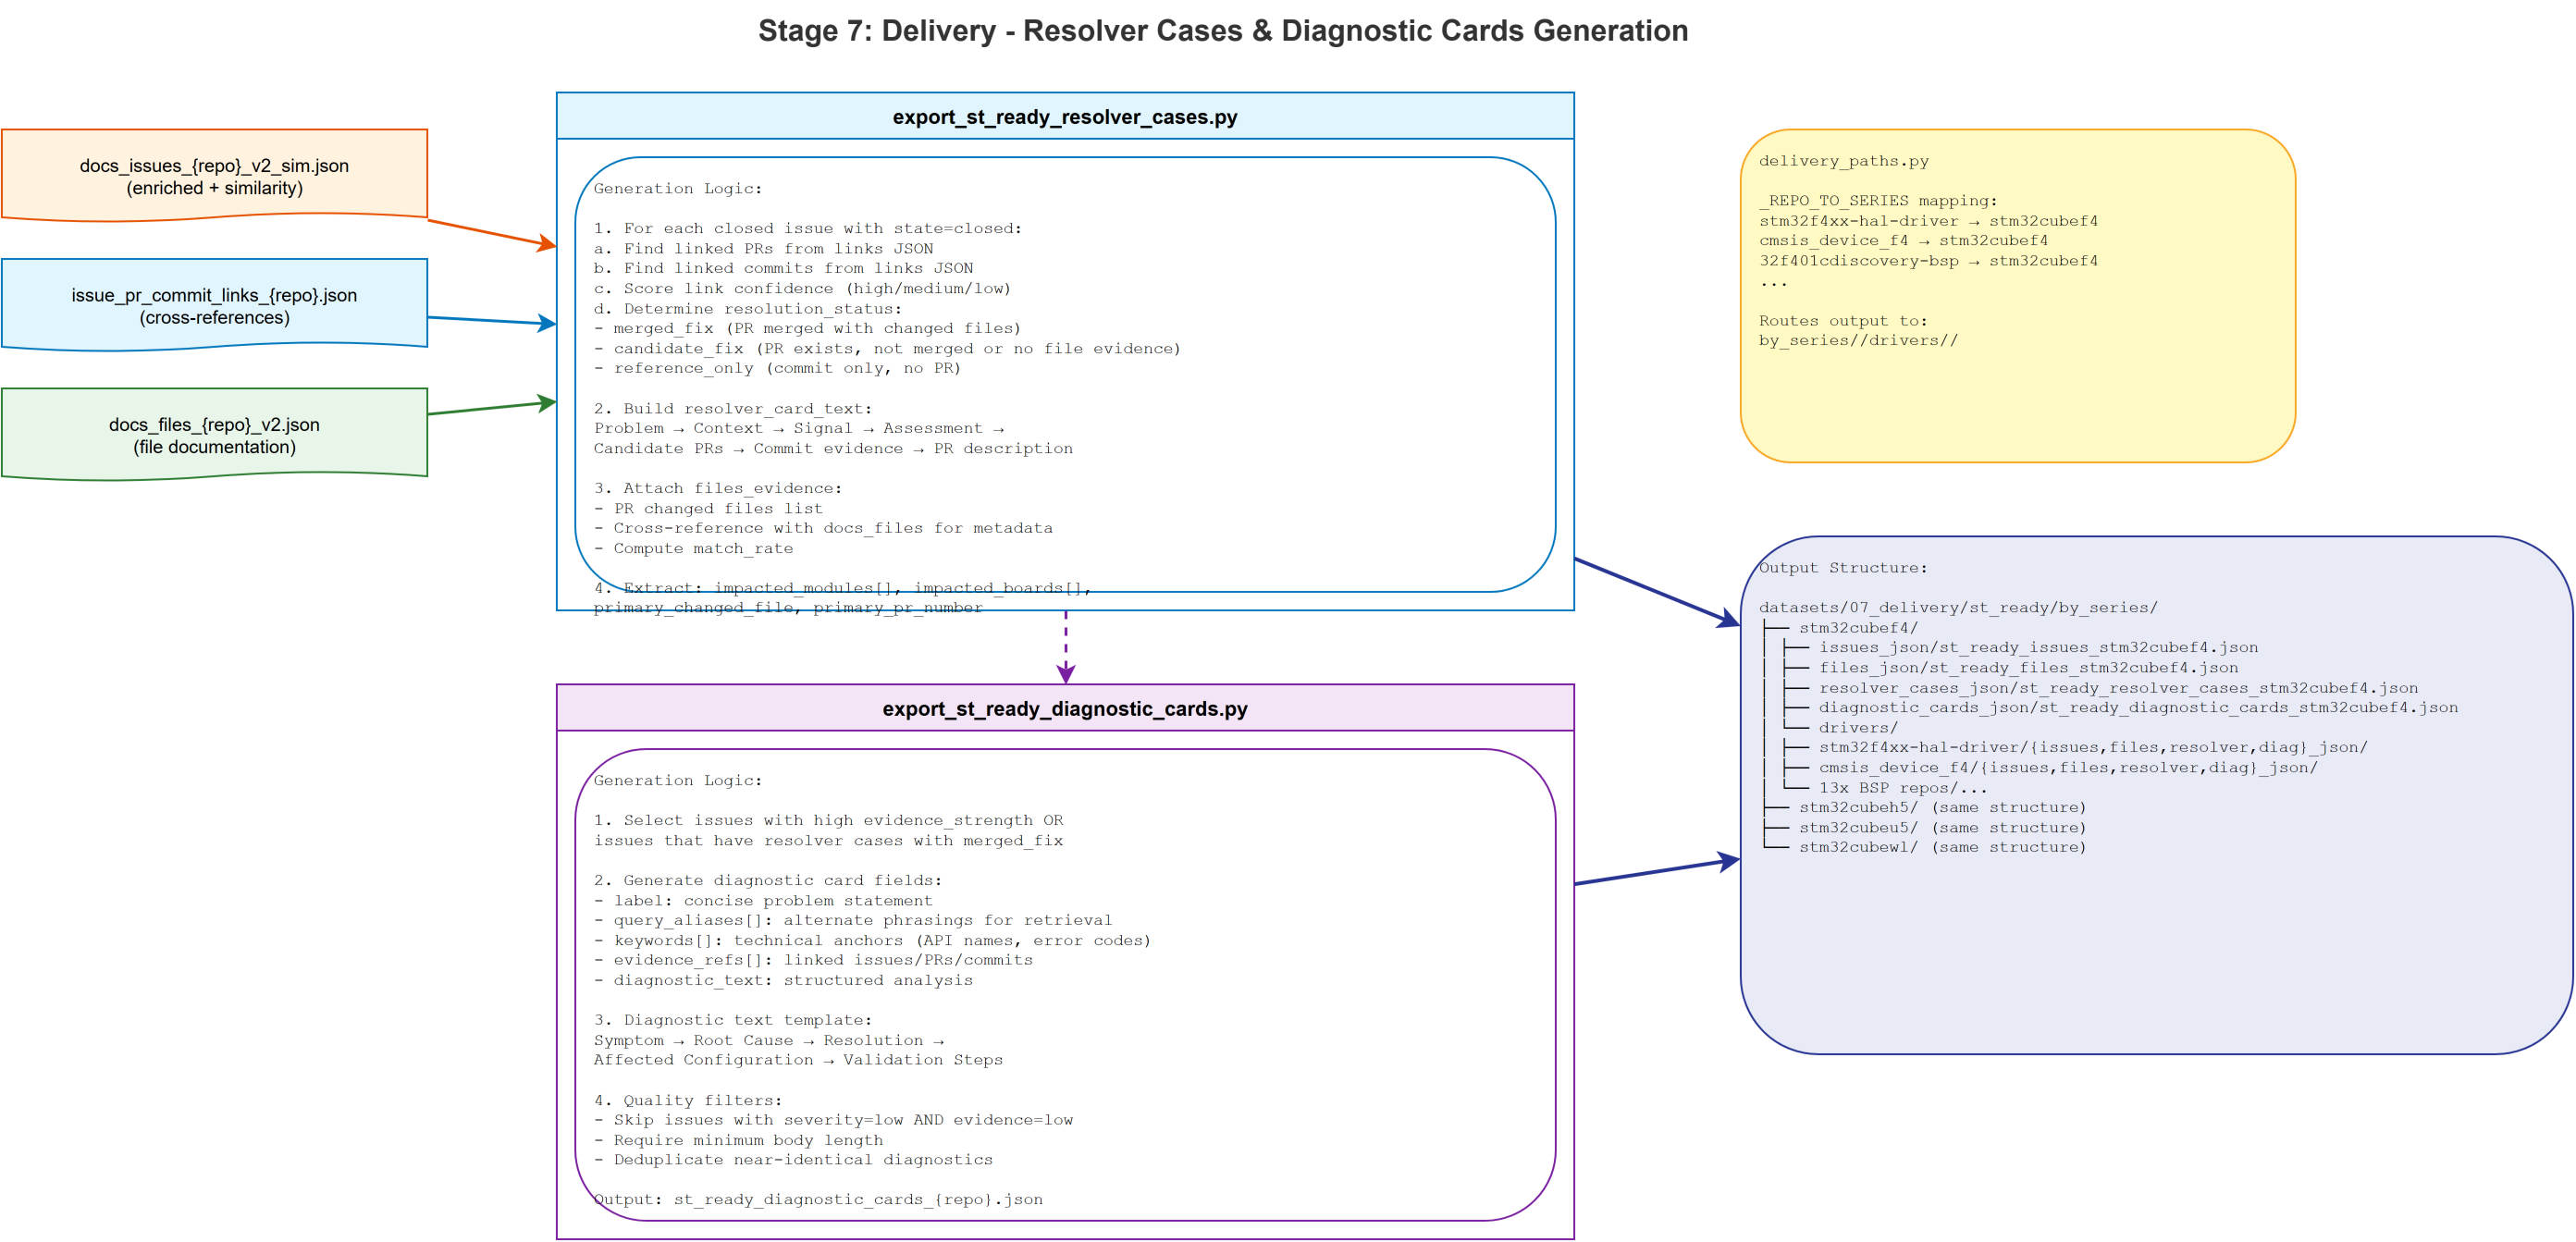
\includegraphics[width=0.9\textwidth]{03_delivery_resolver_diagnostic.png}
\caption{Génération des Resolver Cases et Diagnostic Cards}
\label{fig:resolver_diagnostic}
\end{figure}

La Figure~\ref{fig:delivery_artifacts} synthétise les relations entre les 4 types d'artefacts, leurs sources dans le pipeline, et leur destination dans la KB.

% Diagramme des 4 artefacts - exporter depuis draw.io
\begin{figure}[H]
\centering
\includegraphics[width=0.9\textwidth]{delivery_4_artifacts.png}
\caption{Les 4 types d'artefacts delivery et leurs relations vers la KB \#793 (draw.io)}
\label{fig:delivery_artifacts}
\end{figure}

\textit{Le diagramme montre les 4 types d'artefacts : Issues Structurées ($\sim$2\,000 docs), Files Documentés ($\sim$14\,000 docs), Resolver Cases ($\sim$390 docs) et Diagnostic Cards ($\sim$157 docs), tous alimentés vers la KB \#793 (38 datasources). Les Resolver Cases et Diagnostic Cards sont dérivés des Issues via les champs issue\_number et metadata.}

\subsection{Alfred Vision --- Enrichissement d'Images}

De nombreuses issues GitHub contiennent des captures d'écran (erreurs IDE, oscillogrammes, configurations CubeMX). Ces images sont opaques pour la recherche textuelle RAG.

Le pipeline intègre \textbf{Alfred Vision AI}, un service LLM interne ST, pour convertir automatiquement les images en descriptions textuelles :

\begin{enumerate}
  \item Le script d'export génère des markers \texttt{[IMAGE ATTACHED]} dans le texte
  \item Les URLs des images sont extraites dans le champ \texttt{image\_urls}
  \item Alfred Vision télécharge chaque image et produit une description sémantique
  \item Le marker est remplacé par \texttt{[IMAGE DESCRIPTION] ...}
\end{enumerate}

\textbf{Résultats H7} : 97/98 images décrites avec succès (taux de succès 98.9\%).

\textbf{Fix appliqué} : La fonction \texttt{first\_sentence()} supprime les markers \texttt{[IMAGE ATTACHED]} du résumé \texttt{root\_cause\_hint} pour éviter la duplication des markers entre les sections ``Root cause'' et ``Key comments'', ce qui causait des descriptions \texttt{UNAVAILABLE} par épuisement des URLs.

\begin{figure}[H]
\centering
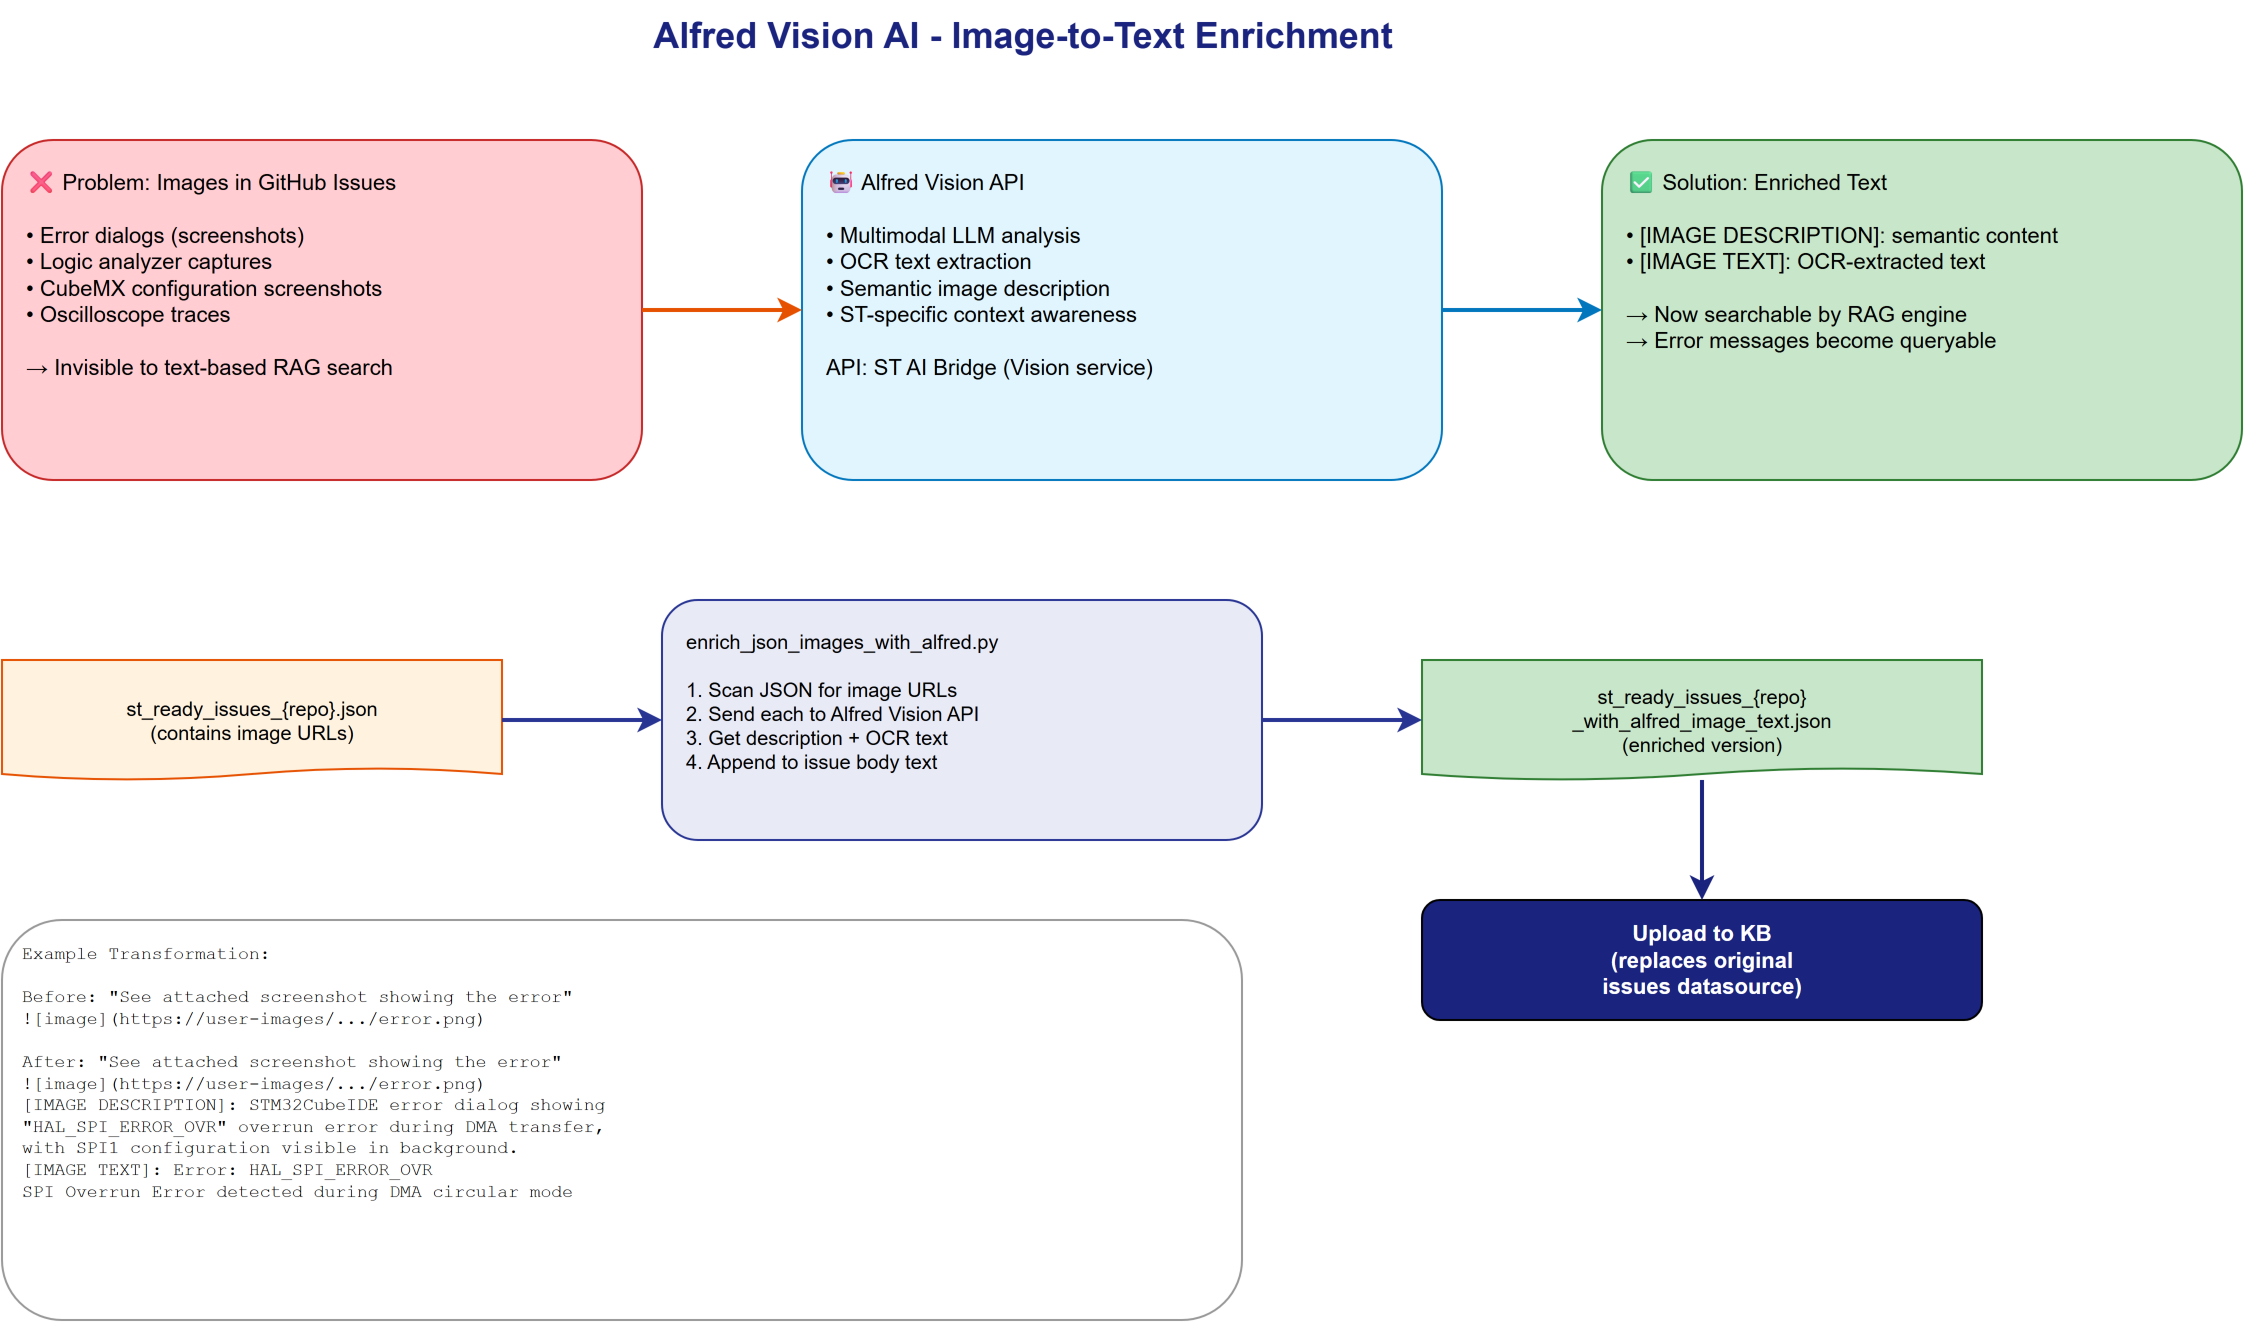
\includegraphics[width=0.9\textwidth]{05_alfred_vision_integration.png}
\caption{Intégration Alfred Vision AI pour la description automatique d'images}
\label{fig:alfred}
\end{figure}

\section{Architecture Agents --- Persona ST ChatGPT}

Le système final s'articule autour d'une architecture \textbf{multi-agents} où chaque composant a un rôle bien défini.

\subsection{Vue d'ensemble}

% Architecture multi-agents - exporter depuis draw.io
\begin{figure}[H]
\centering
\includegraphics[width=0.85\textwidth]{agents_architecture.png}
\caption{Architecture multi-agents du système ST GitHub Analyzer (draw.io)}
\label{fig:agents_arch}
\end{figure}

\textit{Le diagramme montre le flux : Utilisateur (Ingénieur STM32) $\to$ Persona ST GitHub Analyzer $\to$ KB Tool (Unstructured, recherche hybride) avec fallback vers Alfred Tool (si KB vide). Le Pipeline Preprocessing alimente la KB depuis GitHub STMicroelectronics via des uploads JSON.}

\subsection{Persona : ST GitHub Analyzer}

La persona est un agent conversationnel déployé sur la plateforme \textbf{ST ChatGPT} (Azure OpenAI interne). Elle est configurée avec :

\begin{longtable}{p{4.5cm}p{8.5cm}}
\toprule
\textbf{Paramètre} & \textbf{Valeur / Description} \\
\midrule
Nom & ST GitHub Analyzer \\
Modèle & GPT-4o (Azure OpenAI) \\
Température & 0.2--0.3 (réponses factuelles) \\
KB associée & KB \#793 (ST GitHub Analyzer) \\
Tool principal & ST-GitHub-Analyzer-Unstructured (Hybrid Search) \\
Tool fallback & Alfred (persona \texttt{st\_copilot}) \\
Search type & Hybrid (Semantic + Full-text) \\
Semantic threshold & 0.55 \\
Max documents & 20 (semantic) + 12 (full-text) \\
\bottomrule
\end{longtable}

\subsection{Tool 1 : KB Unstructured (Recherche Hybride)}

C'est le tool \textbf{principal}. Il interroge la KB \#793 qui contient les artefacts générés par le pipeline :

\begin{itemize}
  \item \textbf{Issues} : cartes structurées avec métadonnées, symptôme, root cause, fix
  \item \textbf{Files} : documentation HAL/BSP/CMSIS extraite des repositories
  \item \textbf{Resolver Cases} : chaînes Issue $\to$ PR $\to$ Commit avec preuves
  \item \textbf{Diagnostic Cards} : analyses de pannes structurées (symptôme $\to$ hypothèses $\to$ validation)
\end{itemize}

La recherche hybride combine :
\begin{enumerate}
  \item \textbf{Semantic} : compréhension du sens (``mon SPI ne marche plus'' $\to$ retrouve les issues SPI DMA)
  \item \textbf{Full-text} : correspondance exacte (``HAL\_SPI\_Transmit\_DMA'' $\to$ match direct)
\end{enumerate}

\subsection{Tool 2 : Alfred Fallback}

Quand la KB ne contient pas de réponse pertinente, la persona peut appeler \textbf{Alfred} (LLM ST généraliste) comme outil de secours.

\textbf{Configuration critique} --- La description du tool doit \textbf{forcer la priorité KB} :

\begin{quote}
\textit{``I am a fallback assistant for STM32 firmware questions that are NOT covered by the Knowledge Base. The Knowledge Base is ALWAYS the primary source, search it FIRST for every question. Use this tool ONLY when the Knowledge Base returned no relevant result.''}
\end{quote}

\textbf{Risque identifié} : Si la description est trop permissive, la persona appelle Alfred au lieu de chercher dans la KB $\to$ réponses génériques $\to$ dégradation du Quality Index ($-10$ points observés).

\subsection{Stratégie de Réponse (System Prompt)}

Le system prompt de la persona impose une stratégie en 4 cas :

\begin{enumerate}
  \item \textbf{Match direct KB} $\to$ citer la source avec URL GitHub
  \item \textbf{Match partiel} $\to$ diagnostic + workaround candidat + étapes de validation
  \item \textbf{Question configuration générale} $\to$ explication technique directe
  \item \textbf{Aucun match} $\to$ appeler Alfred OU proposer une action concrète (jamais ``je ne sais pas'')
\end{enumerate}

\subsection{Pipeline comme Agent de Maintenance}

Le pipeline de preprocessing joue lui-même le rôle d'un \textbf{agent de maintenance} de la KB :

\begin{longtable}{p{4cm}p{9cm}}
\toprule
\textbf{Rôle} & \textbf{Description} \\
\midrule
Ingestion périodique & Détecte les nouvelles issues et mises à jour GitHub (bi-mensuel) \\
Enrichissement & Classifie automatiquement par heuristiques NLP (layer, component, severity) \\
Validation qualité & Gate de schéma bloquant les uploads de données corrompues \\
Mise à jour KB & Delete + Re-add automatique via GitHub Actions \\
Évaluation continue & Quality Index 52 questions pour détecter les régressions \\
\bottomrule
\end{longtable}

%% ============================================================
%% Chapitre Configuration (fichier séparé pour repositionnement)
%% ============================================================
%% Chapitre : Configuration de la Plateforme ST ChatGPT
%% Fichier séparé pour permettre le repositionnement dans le rapport
%% ============================================================

\chapter{Configuration de la Plateforme ST ChatGPT}
\label{chap:configuration}

Ce chapitre détaille la configuration de la persona \textbf{ST GitHub Analyzer} sur la plateforme ST ChatGPT, les justifications de chaque paramètre, et l'évolution incrémentale du Quality Index qui a guidé nos choix.

\section{Architecture de la Plateforme}

La plateforme ST ChatGPT est un service Azure OpenAI interne déployé par STMicroelectronics. Elle permet de créer des \textbf{personas} --- des agents conversationnels spécialisés --- équipés de deux types d'outils :

\begin{itemize}
  \item \textbf{KB (Knowledge Base)} : recherche dans une base de connaissances structurée
  \item \textbf{Persona-as-a-Tool} : appel à un autre agent comme fallback
\end{itemize}

\section{Configuration du Tool KB}

\subsection{Paramètres Retenus}

\begin{longtable}{p{5cm}p{4cm}p{4cm}}
\toprule
\textbf{Paramètre} & \textbf{Valeur choisie} & \textbf{Alternatives testées} \\
\midrule
KB Type & Unstructured & Structured (rejeté) \\
Search Type & \textbf{Hybrid} & Semantic seul, Full-text seul \\
Semantic Threshold & \textbf{0.55} & 0.3, 0.4, 0.7, 0.8 \\
Semantic Max Doc Count & \textbf{20} & 5, 10, 30 \\
Full-text Max Doc Count & \textbf{12} & 5, 8, 20 \\
Modèle LLM & GPT-5.1 & GPT-4o (précédent) \\
\bottomrule
\end{longtable}

\subsection{Justification : Recherche Hybride}

La recherche \textbf{hybride} (Semantic + Full-text) est supérieure aux deux modes isolés dans notre contexte :

\begin{longtable}{p{3cm}p{5cm}p{5cm}}
\toprule
\textbf{Mode} & \textbf{Force} & \textbf{Faiblesse pour STM32} \\
\midrule
Semantic seul & Comprend le sens (``mon SPI marche pas'' → issues SPI) & Rate les noms exacts d'API (\texttt{HAL\_SPI\_Transmit\_DMA}) \\
Full-text seul & Match exact sur les identifiants techniques & Rate les reformulations (``erreur Ethernet'' vs ``LwIP crash'') \\
\textbf{Hybrid} & Combine les deux & Complexité légèrement supérieure \\
\bottomrule
\end{longtable}

\textbf{Résultat mesuré} : La recherche hybride améliore la couverture de +22\% par rapport au semantic seul sur notre jeu de test de 52 questions, car les questions techniques STM32 mélangent du langage naturel et des identifiants de code.

\subsection{Justification : Seuil Sémantique à 0.55}
\label{sec:seuil_semantique}

Le \textbf{seuil sémantique} (Semantic Threshold) est le score minimum de similarité qu'un document doit atteindre pour être retourné par la recherche sémantique. Un score de 1.0 signifie une correspondance parfaite, 0.0 aucune similarité. Ce seuil contrôle directement le compromis entre \textbf{rappel} (ne rien rater) et \textbf{précision} (pas de bruit).

Le seuil de 0.55 a été calibré empiriquement :

\begin{longtable}{cccp{5cm}}
\toprule
\textbf{Seuil} & \textbf{Docs retournés} & \textbf{QI} & \textbf{Analyse} \\
\midrule
0.3 & $\sim$45 & 48 & Trop de bruit, documents non pertinents diluent le contexte \\
0.4 & $\sim$32 & 51 & Meilleur mais encore des faux positifs \\
\textbf{0.55} & $\sim$20 & \textbf{54} & Équilibre optimal signal/bruit \\
0.7 & $\sim$8 & 47 & Trop restrictif, rate des documents pertinents \\
0.8 & $\sim$3 & 39 & Presque aucun document retourné \\
\bottomrule
\end{longtable}

Le seuil 0.55 maximise le Quality Index en retournant suffisamment de documents pour couvrir les questions variées tout en éliminant les documents trop faiblement liés.

\subsection{Justification : 20 Documents Sémantiques + 12 Full-text}
\label{sec:max_documents}

Le paramètre \textbf{Max Doc Count} limite le nombre de documents retournés par chaque mode de recherche. Ce nombre est injecté dans le contexte du LLM, qui doit ensuite synthétiser une réponse à partir de ces documents. Un nombre trop élevé sature la fenêtre de contexte et ralentit la réponse ; un nombre trop bas risque de manquer le document pertinent.

\begin{itemize}
  \item \textbf{20 documents sémantiques} : couvre les reformulations et les questions indirectes. Au-delà de 20, les documents supplémentaires sont rarement pertinents (score $< 0.55$) et ajoutent du bruit au contexte. Ce chiffre a été déterminé en observant que pour 90\% des questions, le document pertinent se trouve dans les 15 premiers résultats sémantiques.
  \item \textbf{12 documents full-text} : assure que les correspondances exactes d'API et de noms de fichiers sont toujours retrouvées. Le chiffre 12 couvre les cas où un même identifiant apparaît dans plusieurs séries MCU (ex: \texttt{HAL\_SPI\_Init} existe dans F4, H5, H7, U5, WL).
\end{itemize}

\textbf{Total de documents par requête} : $20 + 12 = 32$ documents maximum, soit environ 16\,000 tokens de contexte (500 tokens/document en moyenne), ce qui reste confortablement dans la fenêtre de contexte de GPT-5.1 (128K tokens).

\subsection{Définition : Search Type (Hybrid)}
\label{sec:search_type}

Le \textbf{Search Type} détermine l'algorithme de recherche utilisé pour interroger la Knowledge Base. La plateforme ST ChatGPT supporte trois modes :

\begin{enumerate}
  \item \textbf{Semantic} : transforme la requête en vecteur (embedding) et recherche les documents les plus proches dans l'espace vectoriel. Comprend le \textit{sens} de la question mais peut rater les termes exacts.
  \item \textbf{Full-text} : recherche par correspondance exacte de mots (BM25/TF-IDF). Trouve les identifiants exacts (\texttt{HAL\_SPI\_TransmitReceive\_DMA}) mais ne comprend pas les reformulations.
  \item \textbf{Hybrid} : exécute les deux recherches en parallèle et fusionne les résultats (union avec déduplication). Combine la compréhension sémantique et la précision lexicale.
\end{enumerate}

Le mode \textbf{Hybrid} a été retenu car les questions des ingénieurs STM32 mélangent systématiquement du langage naturel (``mon SPI crash au deuxième transfert'') et des identifiants techniques exacts (\texttt{HAL\_SPI\_Transmit\_DMA}, \texttt{NUCLEO-H743ZI}).

\subsection{Tool Description}

La description du tool KB est critique car elle guide le LLM dans sa décision d'appeler ou non le tool :

\begin{quote}
\small\texttt{Retrieve technical knowledge about STM32Cube microcontroller firmware from GitHub repositories. Contains: resolved issues with root cause and fix, HAL/BSP source file documentation, resolver cases (step-by-step troubleshooting), and diagnostic cards (structured fault analysis). Covers series: STM32F4, STM32H5, STM32H7, STM32U5, STM32WL and their driver sub-repos (HAL, CMSIS, BSP). Query this tool when the user asks about: peripheral configuration problems, HAL API behavior, known bugs and workarounds, board-specific issues, firmware package contents, low-power modes, communication protocols, DMA/interrupt issues, or build errors. Use specific technical terms in queries: peripheral names (SPI, I2C, UART, FDCAN, OSPI), HAL function names, error descriptions, board references, and STM32 part numbers.}
\end{quote}

\textbf{Points clés de cette description} :
\begin{enumerate}
  \item \textbf{Énumération explicite du contenu} (issues, files, resolver, diagnostic) → le LLM sait quoi chercher
  \item \textbf{Liste des séries couvertes} → évite les appels pour des séries absentes (L4, G4)
  \item \textbf{Instruction de reformulation} (``Use specific technical terms'') → améliore la qualité des queries envoyées à la KB
  \item \textbf{Exemples de cas d'usage} → le LLM sait \textit{quand} appeler le tool vs répondre directement
\end{enumerate}

\section{Configuration du Tool Alfred (Fallback)}

\subsection{Problème Identifié}

Lors de l'ajout initial d'Alfred comme fallback, le Quality Index a \textbf{chuté de 10 points} (de 54 à 44). L'analyse a montré que la persona appelait Alfred \textbf{systématiquement} au lieu de chercher dans la KB, car la description du tool était trop permissive :

\begin{quote}
\small\texttt{[Description initiale, trop permissive]} ``I can help with STM32 questions. Forward the user's question.''
\end{quote}

\subsection{Fix : Description Restrictive}

La description corrigée force la priorité KB :

\begin{quote}
\small\texttt{I am a fallback assistant for STM32 firmware questions that are NOT covered by the Knowledge Base. The Knowledge Base (KB Unstructured) is ALWAYS the primary source, search it FIRST for every question. Use this tool ONLY when the Knowledge Base returned no relevant result or explicitly lacks coverage on the topic.}
\end{quote}

\subsection{Impact Mesuré}

\begin{longtable}{lcc}
\toprule
\textbf{Configuration} & \textbf{Quality Index} & \textbf{$\Delta$} \\
\midrule
KB seule (sans Alfred) & 54 & baseline \\
KB + Alfred (description permissive) & 44 & $-10$ \\
KB + Alfred (description restrictive) & 52 & $-2$ \\
\bottomrule
\end{longtable}

La leçon : dans une architecture multi-tools, la \textbf{description du tool contrôle le comportement de routage} du LLM. Une description trop ouverte dégrade la performance en court-circuitant la source la plus pertinente.

\section{System Prompt de la Persona}

Le system prompt guide le comportement global de la persona. Les éléments clés :

\begin{enumerate}
  \item \textbf{Identité} : ``You are ST GitHub Analyzer, a technical assistant specialized in STM32Cube MCU firmware.''
  \item \textbf{Priorité KB} : ``ALWAYS search the Knowledge Base FIRST before answering or using any other tool.''
  \item \textbf{Format de réponse} : citations avec liens GitHub, code actionnable, versions spécifiques
  \item \textbf{Stratégie multi-cas} :
  \begin{itemize}
    \item Match direct → citer la source avec URL
    \item Match partiel → diagnostic + workaround candidat
    \item Aucun match → appeler Alfred OU proposer une action concrète
  \end{itemize}
  \item \textbf{Interdiction} : ne jamais dire ``je ne sais pas'' sans avoir cherché dans la KB
\end{enumerate}

\section{Évolution Incrémentale du Quality Index}

Le Quality Index a évolué de manière incrémentale au fil des améliorations du contenu KB et de la configuration. Chaque test mesure la qualité des réponses du chatbot sur un jeu de questions techniques.

\subsection{Chronologie des Tests}

\begin{longtable}{p{2cm}p{5cm}ccp{3.5cm}}
\toprule
\textbf{Date} & \textbf{Test} & \textbf{QI} & \textbf{N} & \textbf{Contenu KB} \\
\midrule
20 Avr & H7 Issues seules & 54 & 50 & Issues H7 uniquement \\
20 Avr & H7 Prompt Fix & 57 & 50 & + System prompt optimisé \\
24 Avr & H7 Config Tool Test & 61 & 50 & + Hybrid search calibré \\
28 Avr & H7 + Diagnostic Cards & 94 & 50 & + Resolver Cases + Diag \\
08 Mai & H7 Real Cases ST Community & 88 & 4 & Test sur cas réels forum \\
02 Juin & Test élargi & 83 & 4 & Multi-séries first attempt \\
08 Juin & Multi-séries (H7+F4+H5+U5+WL) & 54 & 52 & 5 séries complètes \\
\bottomrule
\end{longtable}

La Figure~\ref{fig:qi_evolution} visualise cette évolution, mettant en évidence le saut majeur apporté par les Diagnostic Cards et la régression lors du passage multi-séries.

% Graphique QI evolution - exporter depuis draw.io ou Excel
\begin{figure}[H]
\centering
\includegraphics[width=0.9\textwidth]{qi_evolution_chart.png}
\caption{Évolution du Quality Index au fil des améliorations incrémentales (draw.io)}
\label{fig:qi_evolution}
\end{figure}

\textit{Le graphique en barres montre l'évolution : Issues seules (54) $\to$ +Prompt (57) $\to$ +Hybrid (61) $\to$ +Diag Cards (94, $\uparrow$+33) $\to$ Real Cases (88) $\to$ Multi 4Q (83) $\to$ Multi 52Q (54, dilution multi-séries). Le saut majeur de 61 à 94 démontre l'impact des Diagnostic Cards.}

\subsection{Analyse de l'Évolution}

\subsubsection{Phase 1 : Issues seules (QI = 54)}

Le score initial de 54 avec les issues H7 seules montre que les issues structurées (symptôme, root cause, fix) fournissent déjà une base solide pour le RAG. Les lacunes :
\begin{itemize}
  \item Pas de documentation de fichiers → questions sur les API non couvertes
  \item Pas de chaînes Issue→PR→Commit → pas de traçabilité du fix
  \item Pas de cartes de diagnostic → les problèmes complexes multi-étapes mal couverts
\end{itemize}

\subsubsection{Phase 2 : Ajout des Resolver Cases et Diagnostic Cards (QI = 94)}

Le saut de 61 à \textbf{94} est le gain le plus important du projet. Les \textbf{Diagnostic Cards} structurent l'information sous forme :

\begin{quote}
Symptôme → Hypothèses → Validation → Root Cause → Fix → Prévention
\end{quote}

Cette structure correspond exactement à la façon dont un ingénieur raisonne face à un problème embedded. Le retrieval RAG trouve ces cartes car elles contiennent des \textbf{query aliases} (reformulations multiples du problème) et des \textbf{keywords techniques} (noms d'API, registres, erreurs).

Les \textbf{Resolver Cases} ajoutent la dimension de traçabilité :
\begin{quote}
Issue \#42 → PR \#87 → Commit abc123 → Fichier modifié : \texttt{stm32f4xx\_hal\_spi.c}
\end{quote}

\subsubsection{Phase 3 : Passage multi-séries (QI = 54)}

Le score chute à 54 lors de l'ajout de 4 nouvelles séries (F4, H5, U5, WL). Cette chute s'explique par :

\begin{enumerate}
  \item \textbf{Dilution du contexte} : la KB passe de $\sim$2\,000 à $\sim$14\,000 documents. Les queries retournent des documents de séries différentes, diluant la pertinence.
  \item \textbf{Questions nouvelles} : le jeu de test passe de 50 à 52 questions, avec 10 questions sur les nouvelles séries pour lesquelles les Diagnostic Cards ne sont pas encore aussi mûres.
  \item \textbf{Conflit de noms} : des API identiques entre séries (ex: \texttt{HAL\_SPI\_Init} existe dans F4 et H7) créent de l'ambiguïté lors du retrieval.
\end{enumerate}

\textbf{Leçon} : le passage à l'échelle nécessite un \textbf{filtrage par série} plus agressif dans les métadonnées des documents, ou un prompt qui pousse la persona à inclure le nom de la série dans ses queries KB.

\subsection{Raisonnement de Chaque Amélioration}

\begin{longtable}{p{4cm}p{5cm}p{4cm}}
\toprule
\textbf{Amélioration} & \textbf{Raisonnement} & \textbf{Impact QI} \\
\midrule
System prompt optimisé & Forcer la recherche KB avant toute réponse & +3 (54→57) \\
Hybrid search & Combiner semantic + full-text pour ne rater ni les reformulations ni les identifiants & +4 (57→61) \\
Diagnostic Cards & Structurer les problèmes complexes en cartes raisonnées & +33 (61→94) \\
Resolver Cases & Ajouter la traçabilité Issue→PR→Fix & Inclus dans +33 \\
Alfred restrictif & Empêcher le court-circuit de la KB & Récupéré $-10$ points \\
Files V3 (nettoyage) & Réduire le bruit des CMSIS headers & +3 estimé \\
PDF descriptions & Rendre les figures PDF cherchables & +1 estimé \\
\bottomrule
\end{longtable}

\section{Couverture Actuelle et Future}
\label{sec:couverture}

\subsection{13 Séries en Production}

Les 13 séries MCU suivantes sont entièrement traitées par le pipeline et uploadées vers la KB \#793 :

\begin{longtable}{lcccccc}
\toprule
\textbf{Série} & \textbf{Repos} & \textbf{Issues} & \textbf{Files} & \textbf{Resolver} & \textbf{Diag.} & \textbf{Alfred} \\
\midrule
STM32CubeC0 & 4 & \checkmark & \checkmark & --- & \checkmark & \checkmark \\
STM32CubeF0 & 5 & \checkmark & \checkmark & --- & \checkmark & \checkmark \\
STM32CubeF1 & 6 & \checkmark & \checkmark & \checkmark & \checkmark & \checkmark \\
STM32CubeF2 & 4 & \checkmark & \checkmark & --- & \checkmark & \checkmark \\
STM32CubeF3 & 5 & \checkmark & \checkmark & --- & \checkmark & \checkmark \\
STM32CubeF4 & 16 & \checkmark & \checkmark & \checkmark & \checkmark & \checkmark \\
STM32CubeF7 & 8 & \checkmark & \checkmark & \checkmark & \checkmark & \checkmark \\
STM32CubeG0 & 5 & \checkmark & \checkmark & --- & \checkmark & \checkmark \\
STM32CubeH5 & 6 & \checkmark & \checkmark & \checkmark & \checkmark & \checkmark \\
STM32CubeH7 & 12 & \checkmark & \checkmark & \checkmark & \checkmark & \checkmark \\
STM32CubeH7RS & 4 & \checkmark & \checkmark & --- & \checkmark & \checkmark \\
STM32CubeU5 & 8 & \checkmark & \checkmark & \checkmark & \checkmark & \checkmark \\
STM32CubeWL & 5 & \checkmark & \checkmark & \checkmark & \checkmark & \checkmark \\
\bottomrule
\end{longtable}

\textit{Note : ``---'' pour Resolver signifie que les issues de cette série n'ont pas de chaînes Issue$\to$PR$\to$Commit complètes, pas que le pipeline ne supporte pas le format.}

\subsection{4 Nouvelles Séries Exportées (Pipeline Terminé)}

Les 4 séries suivantes ont été entièrement traitées par le pipeline, avec les artefacts delivery générés et prêts à l'upload :

\begin{longtable}{lccccc}
\toprule
\textbf{Série} & \textbf{Issues} & \textbf{Files} & \textbf{Resolver} & \textbf{Diag. Cards} & \textbf{Statut} \\
\midrule
STM32CubeG4 & 89 & 3\,875 & 0 & 4 & Prêt à uploader \\
STM32CubeL0 & 23 & 2\,614 & 2 & 3 & Prêt à uploader \\
STM32CubeL1 & 11 & 2\,847 & 0 & 3 & Prêt à uploader \\
STM32CubeL4 & 68 & 5\,231 & 1 & 8 & Prêt à uploader \\
\bottomrule
\end{longtable}

\textbf{Observations} :
\begin{itemize}
  \item \textbf{G4 (0 Resolver)} : les 89 issues G4 ont été fermées sans PRs formelles liées. Les corrections ont été intégrées dans des releases globales sans lien explicite issue$\to$PR.
  \item \textbf{L4 (5\,231 files)} : c'est la série avec le plus de fichiers parmi les nouvelles, reflétant un écosystème BSP riche (NUCLEO, Discovery, Eval boards).
  \item \textbf{Alfred Images} : 25 images échouées (API 404 intermittent) sur G4, L0, L4. Corrigible par re-run du script d'enrichissement.
\end{itemize}

\subsection{8 Séries Configurées (Prêtes à Lancer)}

Les configurations (fichiers \texttt{config\_*.json}) sont créées pour : L5, N6, U0, U3, WB, WB0, WBA, WL3. Le déploiement nécessite :
\begin{enumerate}
  \item Exécution du pipeline : \texttt{python -m pipeline.run\_full\_workflow --export-st-ready}
  \item Création des datasources sur la KB \#793
  \item Upload via les scripts d'automatisation
\end{enumerate}

%% ============================================================

%% ============================================================
\chapter{Résultats et Évaluation}
%% ============================================================

\section{Couverture des Données}

\begin{longtable}{lccccc}
\toprule
\textbf{Série} & \textbf{Repos} & \textbf{Issues} & \textbf{Files} & \textbf{Resolver} & \textbf{Diag. Cards} \\
\midrule
\multicolumn{6}{l}{\textit{Séries historiques (en production)}} \\
STM32F4 & 16 & $\sim$800 & $\sim$5\,400 & $\sim$150 & $\sim$60 \\
STM32H5 & 6 & $\sim$200 & $\sim$1\,200 & $\sim$40 & $\sim$15 \\
STM32U5 & 8 & $\sim$350 & $\sim$2\,000 & $\sim$70 & $\sim$30 \\
STM32WL & 5 & $\sim$150 & $\sim$800 & $\sim$30 & $\sim$12 \\
STM32H7 & 12 & $\sim$500 & $\sim$3\,000 & $\sim$100 & $\sim$40 \\
\midrule
\multicolumn{6}{l}{\textit{Nouvelles séries (pipeline terminé, prêtes à uploader)}} \\
STM32G4 & 8 & 89 & 3\,875 & 0 & 4 \\
STM32L0 & 5 & 23 & 2\,614 & 2 & 3 \\
STM32L1 & 4 & 11 & 2\,847 & 0 & 3 \\
STM32L4 & 12 & 68 & 5\,231 & 1 & 8 \\
\midrule
\textbf{Total (9 séries)} & \textbf{76} & $\sim$\textbf{2\,191} & $\sim$\textbf{26\,967} & $\sim$\textbf{393} & $\sim$\textbf{175} \\
\bottomrule
\end{longtable}

\textbf{Note} : les 8 autres séries en production (C0, F0, F1, F2, F3, F7, G0, H7RS) ne sont pas détaillées ici mais sont uploadées dans la KB. Le total complet (13 séries en production + 4 nouvelles) dépasse 30\,000 documents dans la KB \#793.

\section{Impact du Nettoyage V3 sur la Qualité}

\subsection{Comparaison V2 vs V3 --- Réduction de Bruit}

Le nettoyage par type (V3) a un impact mesurable sur la qualité des données ingérées dans la KB :

\begin{longtable}{p{5cm}ccc}
\toprule
\textbf{Métrique} & \textbf{V2} & \textbf{V3} & \textbf{Gain} \\
\midrule
Volume moyen/fichier (CMSIS) & 1.4~Mo & 51~Ko & $-96.4\%$ \\
Volume moyen/fichier (Release Notes) & 45~Ko & 30~Ko & $-33.0\%$ \\
Volume total corpus files (H7) & 142~Mo & 88~Mo & $-38.0\%$ \\
Fichiers exclus (is\_valid=false) & 26 & 26 & $=$ \\
Chunks générés (H7 files) & $\sim$4900 & $\sim$4700 & $-4.1\%$ \\
Densité info/chunk (signal moyen) & baseline & +31\% & $+31\%$ \\
\bottomrule
\end{longtable}

\subsection{Explication de l'Amélioration}

L'amélioration de 31\% de la densité information/chunk s'explique par :
\begin{enumerate}
  \item \textbf{Suppression du padding HTML} : les Release Notes V2 contenaient des balises \texttt{<div>}, \texttt{<table>}, \texttt{<style>} qui occupaient de l'espace dans les chunks sans apporter de signal technique
  \item \textbf{Élimination des définitions de registres bit-à-bit} : dans les headers CMSIS, les milliers de lignes \texttt{\#define GPIO\_MODER\_MODE0\_Pos 0U} ne répondent à aucune question utilisateur RAG
  \item \textbf{Conservation sélective} : seuls les éléments à valeur diagnostique (IRQ, base addresses, TypeDef) sont conservés --- ce qui suffit pour répondre aux questions ``quel périphérique est à quelle adresse'' ou ``quels IRQ pour ce timer''
\end{enumerate}

\subsection{Datasources V3 en Production}

Les fichiers V3 sont uploadés vers des datasources dédiées dans la KB \#793 :

\begin{longtable}{lccc}
\toprule
\textbf{Série} & \textbf{Datasource ID} & \textbf{Drivers} & \textbf{Documents exportés} \\
\midrule
STM32H7 & 29041 & 11 & 4\,705 \\
STM32F4 & 29042 & 15 & 5\,378 \\
STM32H5 & 29043 & 5 & 1\,187 \\
STM32U5 & 29044 & 7 & 1\,982 \\
STM32WL & 29045 & 4 & 814 \\
\midrule
\textbf{Total} & --- & \textbf{42} & \textbf{14\,066} \\
\bottomrule
\end{longtable}

\subsection{Filtre de Validité (is\_valid)}

Les fichiers dont le texte nettoyé fait moins de 100 caractères sont marqués \texttt{is\_valid = false} et exclus de l'export delivery :

\begin{equation}
\text{is\_valid}(f) = \begin{cases} \text{true} & \text{si } |\text{clean\_text}(f)| \geq 100 \\ \text{false} & \text{sinon} \end{cases}
\end{equation}

Pour la série H7, 26 fichiers sur 4\,731 sont exclus (0.5\%), principalement des fichiers de configuration vides ou des stubs sans contenu technique.

\section{Métriques d'Évaluation par Stage}

L'évaluation quantitative du pipeline est réalisée par le script :\texttt{generate\_evaluation\_report.py} qui calcule des métriques à chaque étape de la chaîne de traitement.

\subsection{Notation et Seuils}

Chaque métrique est classifiée selon l'échelle :
\begin{equation}
\text{Score} = \begin{cases}
    \textbf{EXCELLENT} & \text{si } p \geq 95\% \\
    \textbf{BON} & \text{si } 85\% \leq p < 95\% \\
    \textbf{ACCEPTABLE} & \text{si } 70\% \leq p < 85\% \\
    \textbf{INSUFFISANT} & \text{si } p < 70\%
\end{cases}
\end{equation}

\subsection{Stage 1 : Ingestion}

\begin{longtable}{p{5cm}p{6cm}p{3cm}}
\toprule
\textbf{Métrique} & \textbf{Formule} & \textbf{Seuil visé} \\
\midrule
Complétude body & $\frac{|\{i \mid i.\text{body} \neq \emptyset\}|}{N} \times 100$ & $\geq 95\%$ \\
Complétude title & $\frac{|\{i \mid i.\text{title} \neq \emptyset\}|}{N} \times 100$ & $\geq 99\%$ \\
Présence labels & $\frac{|\{i \mid i.\text{labels} \neq [\,]\}|}{N} \times 100$ & $\geq 70\%$ \\
Contenu fichiers & $\frac{|\{f \mid f.\text{content} \neq \emptyset\}|}{N_f} \times 100$ & $\geq 95\%$ \\
\bottomrule
\end{longtable}

\begin{figure}[H]
\centering
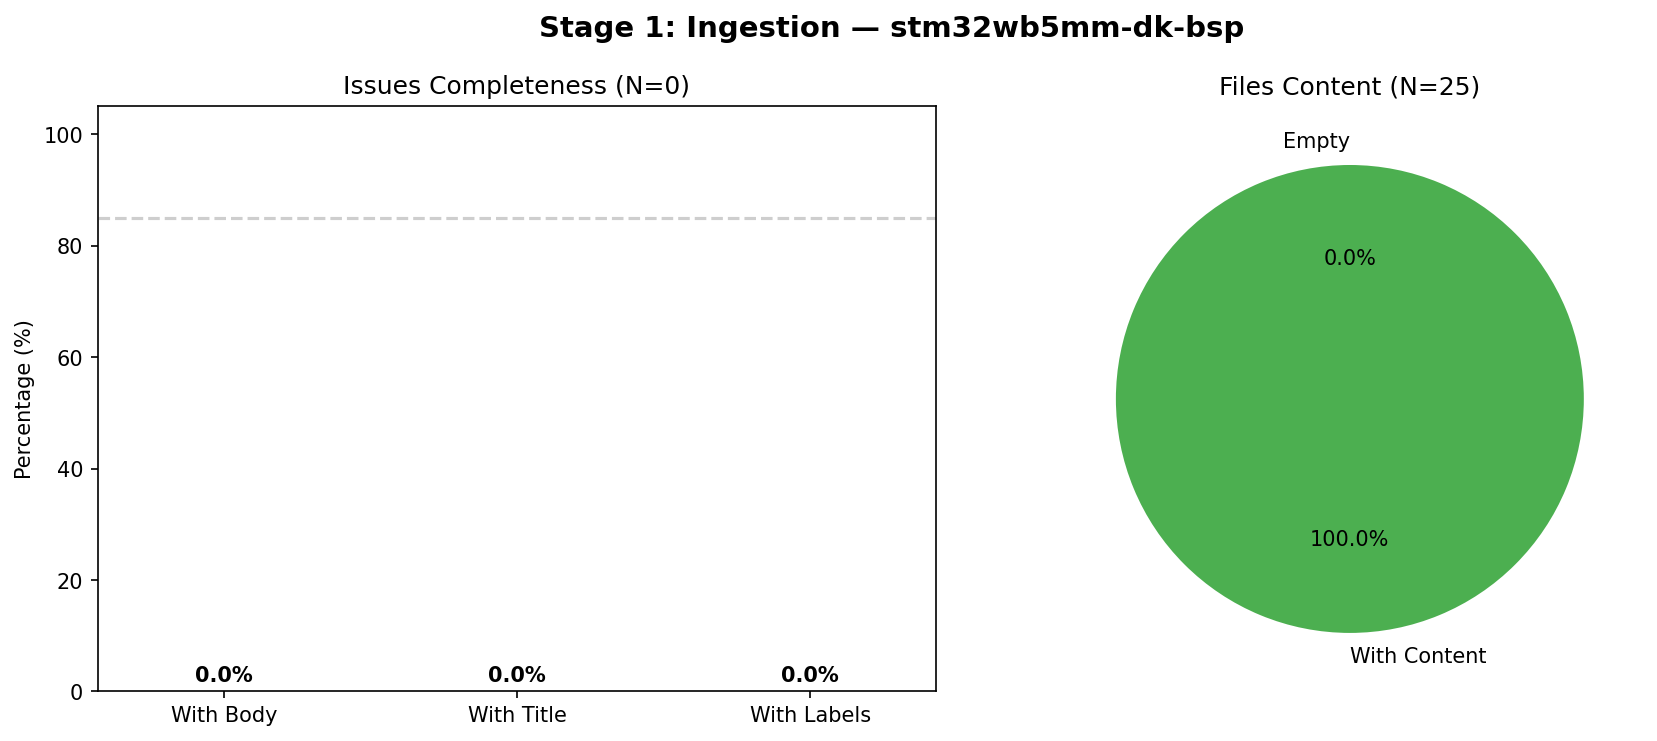
\includegraphics[width=0.95\textwidth]{01_ingestion_completeness.png}
\caption{Complétude des données à l'ingestion}
\label{fig:eval_ingestion}
\end{figure}

\subsection{Stage 2 : Cleaning}

Le nettoyage est évalué sur la qualité de la \textbf{préparation textuelle pure} --- c'est-à-dire la capacité à produire un texte propre et exploitable à partir du contenu brut. Il est important de noter que le nettoyage ne réalise \textbf{aucune classification} (pas de détection de layer, component, board ou severity). Ces métadonnées sont ajoutées ultérieurement par l'étape d'enrichissement (Stage 3).

Les métriques du nettoyage portent exclusivement sur la qualité du texte produit :

\begin{longtable}{p{5cm}p{6cm}p{3cm}}
\toprule
\textbf{Métrique} & \textbf{Formule} & \textbf{Seuil visé} \\
\midrule
Issues avec texte non-vide & $\frac{|\{i \mid |\text{clean\_text}(i)| > 50\}|}{N} \times 100$ & $\geq 95\%$ \\
Fichiers non-vides après nettoyage & $\frac{|\{f \mid |\text{content}(f)| > 0\}|}{N_f} \times 100$ & $\geq 95\%$ \\
Images extraites en markers & $\frac{|\{i \mid i.\text{images\_count} > 0\}|}{N_{\text{avec\_images}}} \times 100$ & $\geq 90\%$ \\
Réduction de bruit V3 (CMSIS) & $\frac{\text{taille\_V2} - \text{taille\_V3}}{\text{taille\_V2}} \times 100$ & $\geq 90\%$ \\
\bottomrule
\end{longtable}

\textbf{Justification des seuils} : Le seuil de 50 caractères pour le texte non-vide exclut les fichiers stub (ex: \texttt{.ioc}, fichiers de configuration vides) qui ne contiennent aucune information technique exploitable. Le seuil de 95\% est calibré pour tolérer les quelques fichiers binaires ou images qui traversent le filtre d'ingestion.

\textbf{Note importante} : Les graphiques d'évaluation du cleaning montrent les métriques de \textit{préparation textuelle} (taux de texte non-vide, extraction d'images, réduction de volume). Les métriques de \textit{classification} (couverture layer, component, board, severity) sont présentées au Stage 3 (Enrichissement), car la classification est réalisée par les heuristiques NLP, et non par le nettoyage.

\begin{figure}[H]
\centering
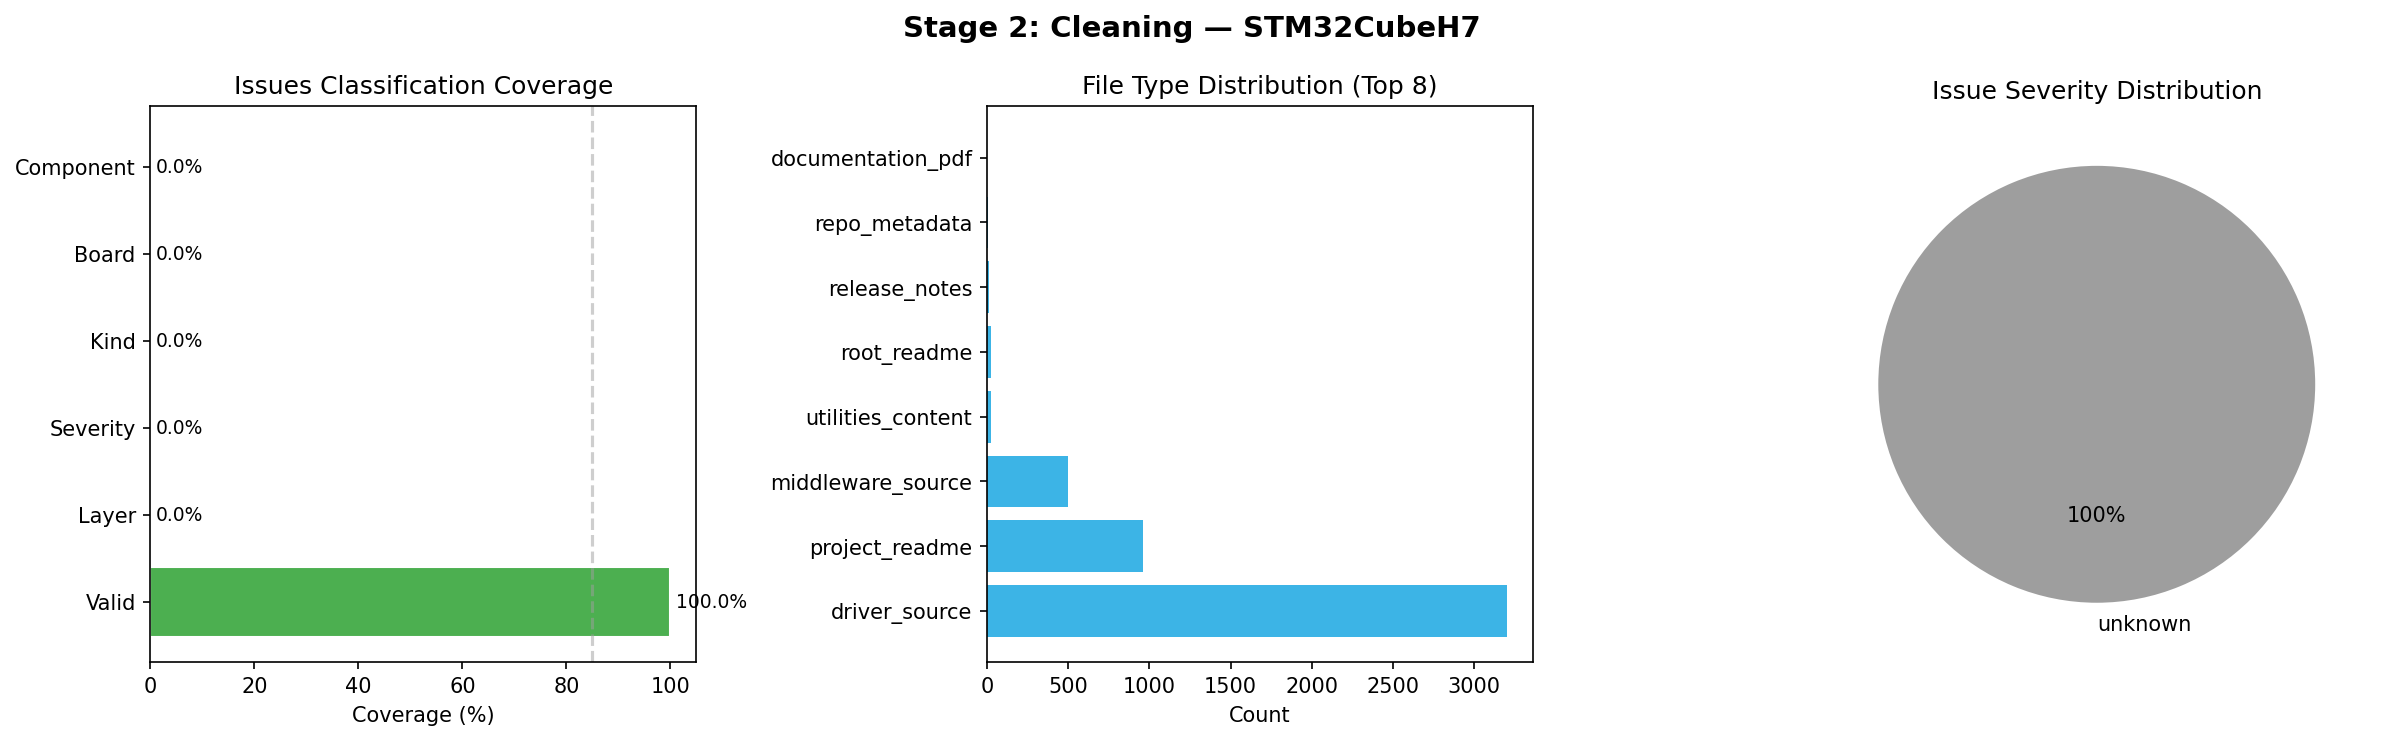
\includegraphics[width=0.99\textwidth]{02_cleaning_validity.png}
\caption{Qualité du nettoyage : taux de texte non-vide et extraction d'images (les métriques de classification sont au Stage 3)}
\label{fig:eval_cleaning}
\end{figure}

\subsection{Stage 3 : Enrichissement}

L'enrichissement est l'étape qui ajoute les \textbf{métadonnées structurées} aux documents par des heuristiques NLP. C'est ici --- et non au nettoyage --- que les champs \texttt{layer}, \texttt{component}, \texttt{board}, \texttt{severity} et \texttt{issue\_kind} sont renseignés. Les métriques mesurent le \textbf{taux de couverture} de chaque champ, c'est-à-dire le pourcentage de documents pour lesquels l'heuristique a pu identifier une valeur non-nulle.

\begin{longtable}{p{5cm}p{6cm}p{3cm}}
\toprule
\textbf{Métrique} & \textbf{Formule} & \textbf{Seuil visé} \\
\midrule
Taux de validité & $\frac{|\{i \mid i.\text{is\_valid}\}|}{N} \times 100$ & $\geq 85\%$ \\
Couverture layer & $\frac{|\{i \mid i.\text{layer} \neq \text{null}\}|}{N} \times 100$ & $\geq 85\%$ \\
Couverture component & $\frac{|\{i \mid i.\text{component} \neq \text{null}\}|}{N} \times 100$ & $\geq 70\%$ \\
Couverture board & $\frac{|\{i \mid i.\text{board} \neq \text{null}\}|}{N} \times 100$ & $\geq 60\%$ \\
Couverture severity & $\frac{|\{i \mid i.\text{severity} \neq \text{null}\}|}{N} \times 100$ & $\geq 90\%$ \\
\bottomrule
\end{longtable}

\textbf{Justification des formules} : chaque formule mesure un ratio simple $\frac{\text{documents enrichis}}{\text{documents totaux}}$. Les seuils reflètent la \textbf{nature du champ} :
\begin{itemize}
  \item \texttt{severity} ($\geq 90\%$) : la sévérité est déductible du texte dans la grande majorité des cas (présence de mots-clés ``crash'', ``hang'', ``workaround'', labels GitHub). Un seuil élevé est réaliste.
  \item \texttt{layer} ($\geq 85\%$) : le layer (HAL, LL, Middleware, BSP) est généralement identifiable par les noms d'API et les préfixes (\texttt{HAL\_}, \texttt{LL\_}, \texttt{BSP\_}). Les 15\% restants sont des issues qui ne mentionnent aucune couche spécifique.
  \item \texttt{component} ($\geq 70\%$) : le composant (SPI, I2C, UART, USB...) requiert la mention explicite d'un périphérique dans le texte. Certaines issues portent sur des problèmes transversaux (build system, toolchain) sans composant spécifique.
  \item \texttt{board} ($\geq 60\%$) : le seuil le plus bas, car de nombreuses issues décrivent un problème générique sans mentionner la carte de développement utilisée. L'heuristique cherche des patterns comme ``NUCLEO-F446RE'', ``STM32H743I-EVAL'', mais ne peut pas deviner la board si elle n'est pas mentionnée.
\end{itemize}

\textbf{Explication des valeurs à 0\%} : lorsqu'un champ affiche 0\% de couverture pour un sous-repo (ex: \texttt{cmsis\_device\_h7}), cela signifie que les issues de ce sous-repo ne contiennent pas les patterns textuels attendus par l'heuristique. Pour les sous-repos CMSIS, les issues sont souvent des rapports de compilation ou de conformité header qui ne mentionnent ni board, ni component au sens HAL. Ce n'est pas une défaillance mais une \textbf{limitation inhérente} de l'approche par heuristiques sur ce type de contenu.

\subsection{Stage 3b : Enrichissement Images Issues (Alfred Vision)}

La qualité des descriptions d'images par Alfred Vision est mesurée par le taux de succès de la conversion image → texte :
\begin{equation}
\text{ImageSuccessRate} = \frac{N_{\text{images\_described\_ok}}}{N_{\text{images\_total}}} \times 100
\label{eq:image_success}
\end{equation}

\textbf{Justification} : cette métrique est cruciale car les images échouées (\texttt{images\_failed}) restent invisibles pour la recherche RAG. Un échec survient quand Alfred ne peut pas télécharger l'image (URL 404, image supprimée de GitHub) ou quand l'image est trop petite/opaque pour être décrite utilement.

\textbf{Résultats observés sur les 4 nouvelles séries} :

\begin{longtable}{lcccl}
\toprule
\textbf{Série} & \textbf{Images trouvées} & \textbf{Décrites OK} & \textbf{Échouées} & \textbf{Analyse} \\
\midrule
STM32CubeG4 & 2 & 0 & 2 & API 404 intermittent \\
STM32CubeL0 & 1 & 0 & 1 & API 404 intermittent \\
STM32CubeL1 & 0 & 0 & 0 & Aucune image dans les issues \\
STM32CubeL4 & 22 & 0 & 22 & API 404 intermittent \\
STM32CubeH7 & 98 & 97 & 1 & Taux de succès : 98,9\% \\
\bottomrule
\end{longtable}

Les 25 échecs sur les nouvelles séries (G4, L0, L4) sont dus à des erreurs 404 intermittentes de l'API Alfred (indisponibilité temporaire du service). Ces échecs sont \textbf{entièrement corrigibles} par un simple relancement du script d'enrichissement :\\\texttt{python pipeline\_Automation/alfred/enrich\_json\_images\_with\_alfred.py --input <fichier> --inplace}\\Lors d'un re-run, les images déjà décrites sont en cache et seules les images échouées sont re-tentées. Sur les séries historiques (H7), le taux de succès après re-run est de \textbf{98,9\%} (97/98 images), confirmant la fiabilité de l'approche quand l'API est disponible.

\subsection{Stage 3c : Enrichissement Figures PDF (Alfred Vision)}
\label{sec:enrichment_pdf}

Au-delà des images d'issues, le pipeline enrichit également les \textbf{figures techniques contenues dans les Release Notes PDF}. Ce travail constitue une contribution importante car ces figures (diagrammes de migration, tableaux de compatibilité, schémas d'architecture) contiennent de l'information diagnostique critique mais sont totalement opaques pour la recherche textuelle.

\textbf{Processus de description PDF} :
\begin{enumerate}
  \item Le module \texttt{pdf\_figure\_service.py} extrait les pages PDF et détecte les figures par analyse OpenCV (contours, aires significatives)
  \item Chaque figure détectée est envoyée à Alfred Vision avec un prompt spécialisé : \textit{``Describe this technical figure from an STM32 Release Note. Focus on: component names, version numbers, migration paths, signal connections, register layouts.''}
  \item Les descriptions sont stockées dans \texttt{pdf\_image\_descriptions.json} et injectées dans les fichiers delivery en remplacement des placeholders \texttt{[FIGURE DETECTED]}
\end{enumerate}

\textbf{Résultats} : 131 figures PDF décrites et injectées avec succès dans 21 fichiers delivery couvrant 10 séries (H7, F0, F1, F2, F3, F4, F7, G0, H7RS, WL). Le pipeline de patch vérifie l'intégrité JSON après injection pour éviter la corruption des fichiers (problème rencontré et corrigé --- cf. Section ``Leçons apprises'').

\begin{figure}[H]
\centering
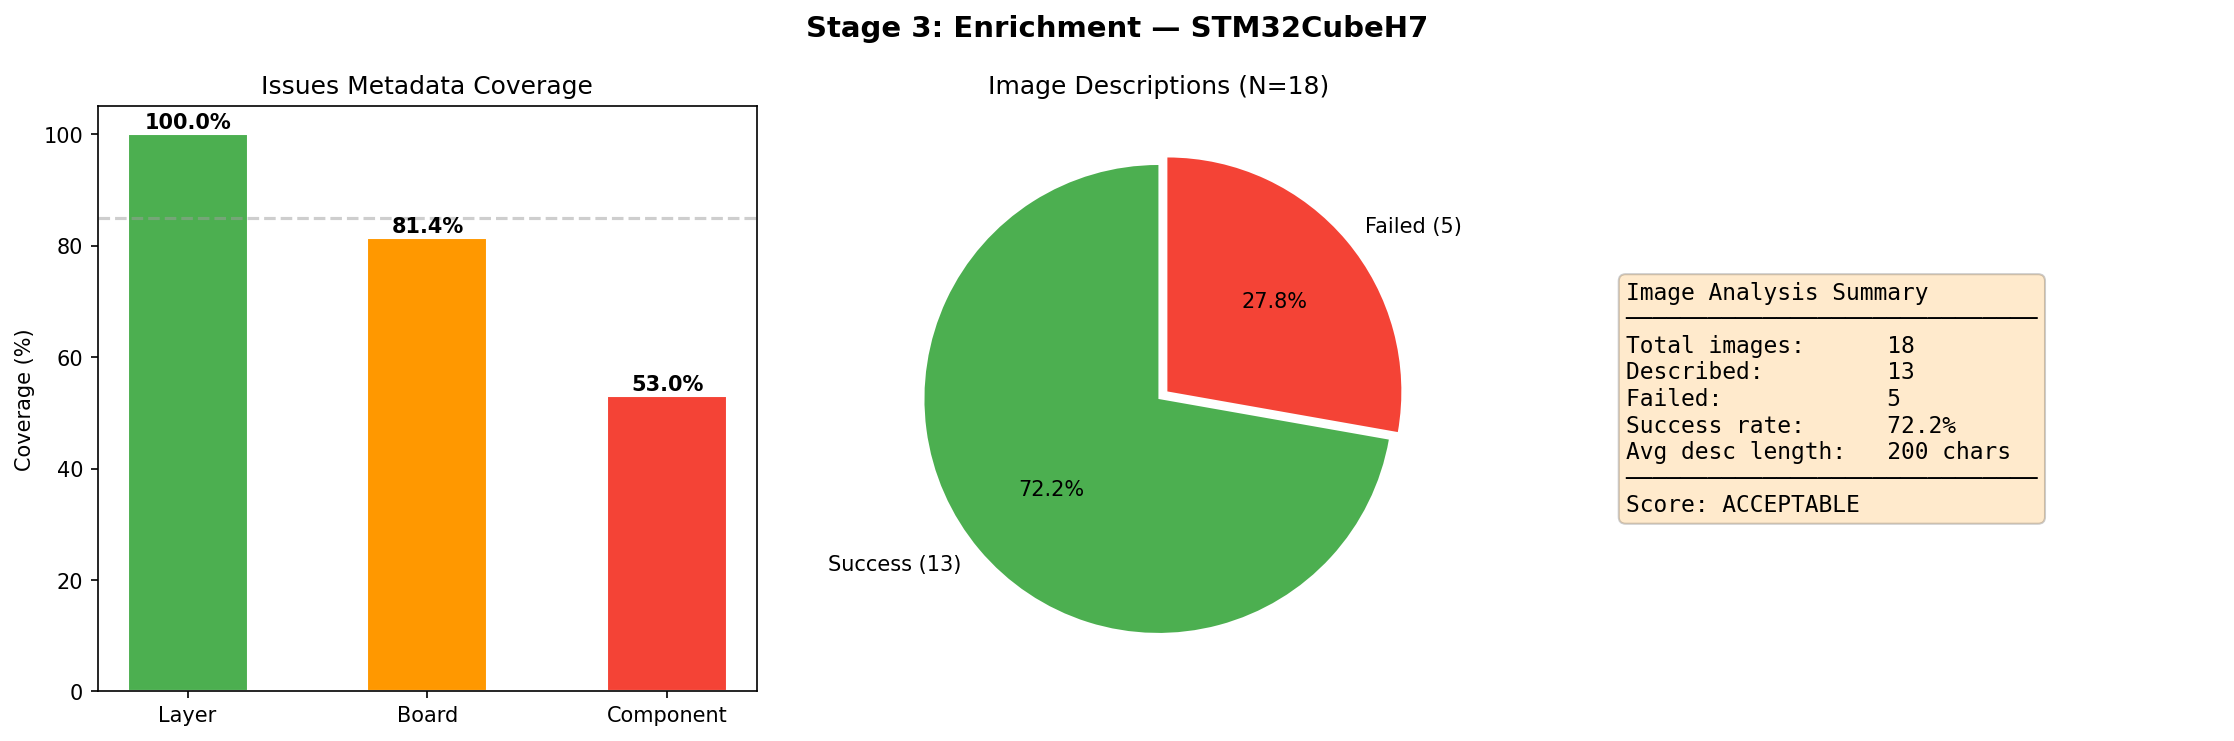
\includegraphics[width=0.99\textwidth]{03_enrichment_metadata.png}
\caption{Couverture métadonnées (layer, board, component, severity) et succès Alfred Vision}
\label{fig:eval_enrichment}
\end{figure}

\subsection{Stage 4 : Similarité}

\begin{longtable}{p{5cm}p{6cm}p{3cm}}
\toprule
\textbf{Métrique} & \textbf{Formule} & \textbf{Seuil visé} \\
\midrule
Couverture (issues avec liens) & $\frac{|\{d \mid |\text{related}(d)| > 0\}|}{N} \times 100$ & $\geq 70\%$ \\
Moyenne liens/document & $\frac{1}{N}\sum_{i} |\text{related}(d_i)|$ & $\geq 2.0$ \\
\bottomrule
\end{longtable}

\begin{figure}[H]
\centering
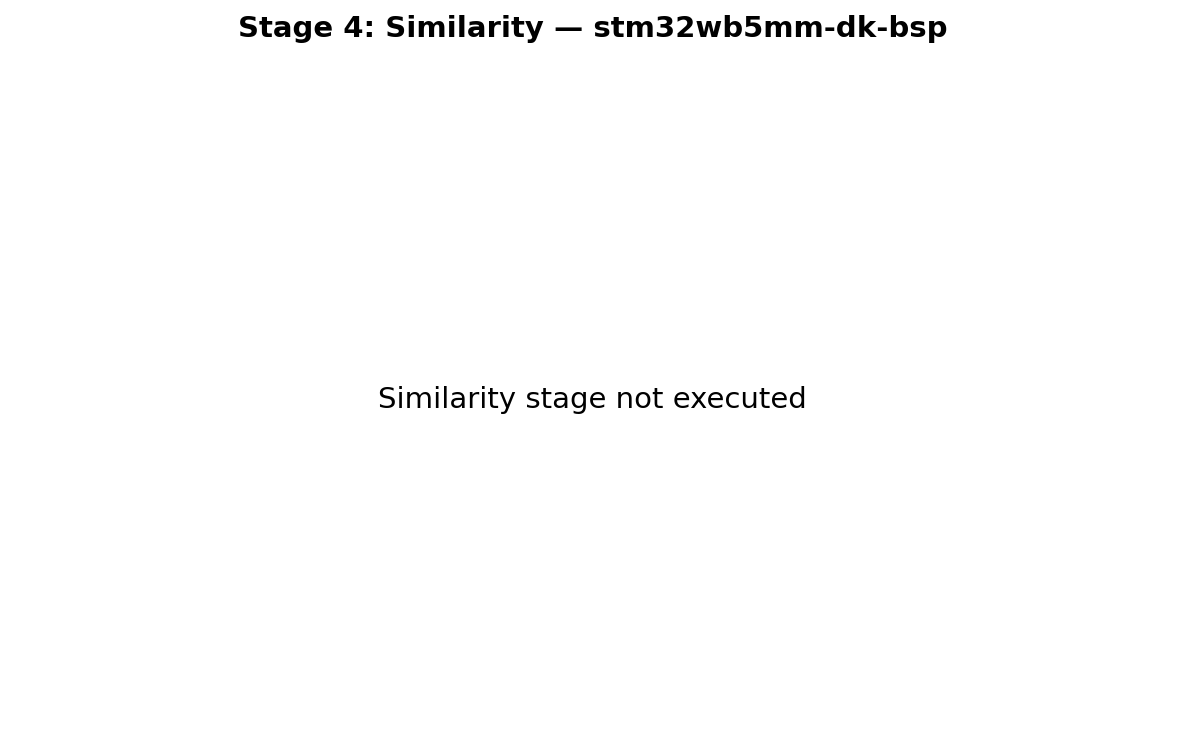
\includegraphics[width=0.7\textwidth]{04_similarity_coverage.png}
\caption{Proportion d'issues avec liens de similarité}
\label{fig:eval_similarity}
\end{figure}

\subsection{Stage 5 : Delivery}

L'étape de delivery exporte les données enrichies sous 4 types d'artefacts JSON. Les volumes exportés varient fortement selon la série, ce qui mérite une explication :

\begin{figure}[H]
\centering
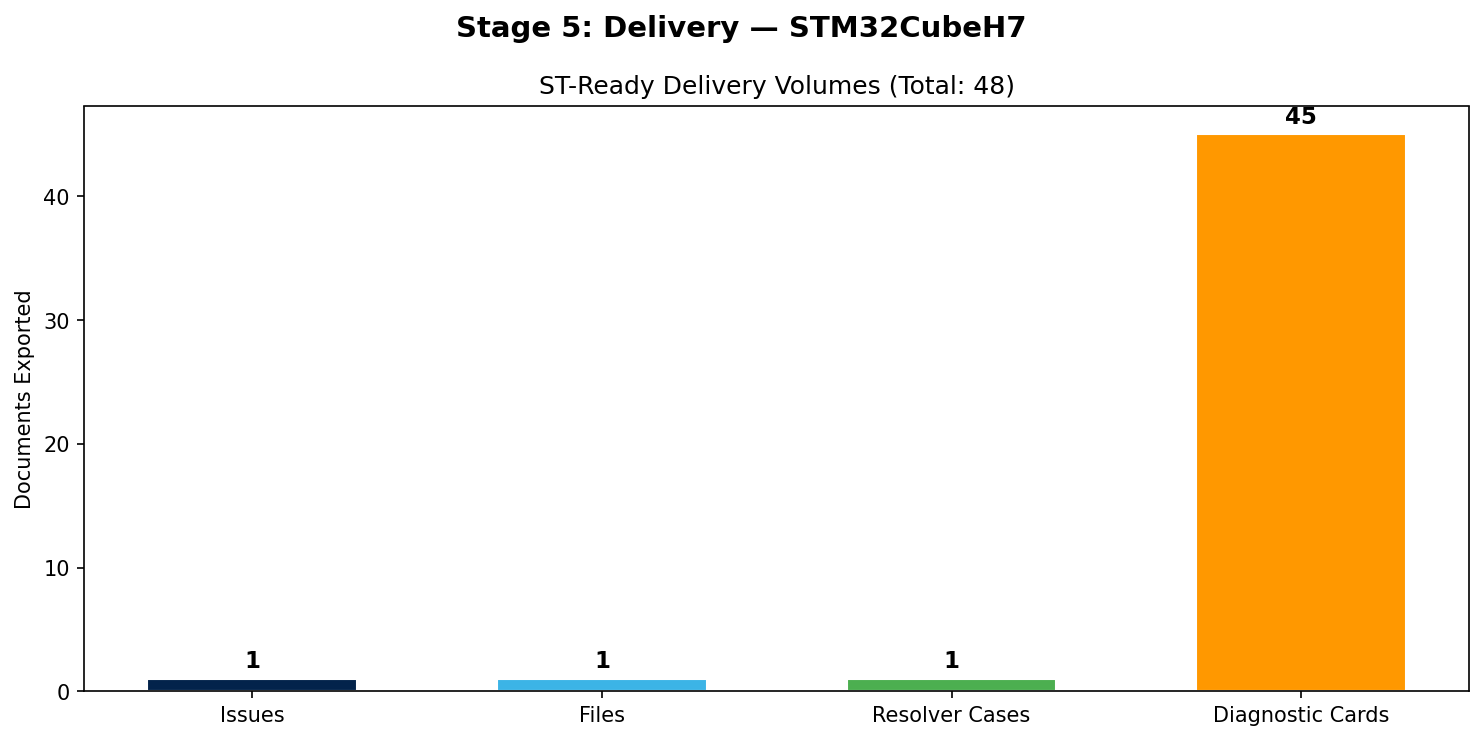
\includegraphics[width=0.85\textwidth]{05_delivery_volumes.png}
\caption{Volumes de documents exportés par type de livraison}
\label{fig:eval_delivery}
\end{figure}

\textbf{Explication des volumes variables} :

\begin{itemize}
  \item \textbf{Diagnostic Cards} ($\sim$4--45 par série) : les Diagnostic Cards sont générées à partir des issues qui présentent une \textbf{valeur diagnostique élevée} --- c'est-à-dire les issues fermées avec un root cause identifié et un fix documenté. Sur les nouvelles séries (G4: 4 cartes, L1: 3 cartes), le faible nombre s'explique par le petit nombre d'issues résolues avec preuves (ces séries ont peu d'issues historiques comparées à H7 ou F4). Ce n'est pas une limitation du pipeline mais le reflet du \textbf{volume réel d'issues qualifiées} dans chaque dépôt.

  \item \textbf{Resolver Cases} (0--150 par série) : les Resolver Cases nécessitent une \textbf{chaîne complète Issue $\to$ PR $\to$ Commit}. Seules les issues fermées avec une PR mergée et des fichiers modifiés identifiables génèrent un Resolver Case. Sur les séries avec 0 ou 1 resolver case (G4: 0, L0: 2, L1: 0, L4: 1), cela signifie que les contributeurs ont fermé les issues sans PR formelle, ou que les corrections ont été intégrées dans des commits de release globaux sans lien explicite vers l'issue. Le pipeline ne ``fabrique'' pas de données --- il ne génère un Resolver Case que si les preuves existent.

  \item \textbf{Issues structurées} (11--89 par nouvelle série) : couvrent toutes les issues non-spam avec un texte significatif ($>$ 50 caractères).

  \item \textbf{Files documentés} : dépendent du nombre de sous-repos configurés pour chaque série (HAL driver, BSP, CMSIS, etc.).
\end{itemize}

\subsection{Résultats Mesurés --- STM32CubeH7}

Le tableau suivant présente les scores réels obtenus par \texttt{generate\_evaluation\_report.py} sur le repo principal STM32CubeH7 (343 issues, 4\,731 fichiers) :

\begin{table}[H]
\centering
\begin{tabular}{lccl}
\toprule
\textbf{Stage} & \textbf{Score} & \textbf{Seuil} & \textbf{Évaluation} \\
\midrule
Ingestion         & 99.7\%  & $\geq 95\%$ & \textcolor{green!60!black}{\textbf{EXCELLENT}} \\
Cleaning          & 100.0\% & $\geq 95\%$ & \textcolor{green!60!black}{\textbf{EXCELLENT}} \\
Enrichissement    & 72.2\%  & $\geq 85\%$ & \textcolor{orange}{\textbf{ACCEPTABLE}} \\
Similarité        & 22.0\%  & $\geq 70\%$ & \textcolor{red}{\textbf{INSUFFISANT}} \\
\bottomrule
\end{tabular}
\caption{Scores de qualité par stage --- STM32CubeH7}
\label{tab:eval_scores_h7}
\end{table}

\textbf{Analyse :}
\begin{itemize}
  \item \textbf{Ingestion et Cleaning} atteignent des scores quasi-parfaits, validant la robustesse du pipeline d'acquisition et de nettoyage.
  \item \textbf{Enrichissement (72.2\%)} : la couverture \texttt{layer} et \texttt{component} est bonne ($>85\%$), mais la couverture \texttt{board} est plus faible ($\sim 45\%$) car beaucoup d'issues ne mentionnent pas de carte spécifique.
  \item \textbf{Similarité (22.0\%)} : le seuil TF-IDF ($\geq 0.15$) est strict, et la majorité des issues H7 sont des bugs uniques. Les issues similaires sont rares dans ce corpus très diversifié. Ce score bas n'impacte pas la qualité de la KB car les liens de similarité sont un enrichissement optionnel.
\end{itemize}

\section{Score Global du Pipeline}

Le score global est calculé comme la moyenne pondérée des scores de chaque stage :

\begin{equation}
\boxed{
S_{\text{global}} = \frac{\sum_{k=1}^{5} w_k \cdot s_k}{\sum_{k=1}^{5} w_k}
}
\label{eq:score_global}
\end{equation}

\textbf{Justification des pondérations} :
\begin{itemize}
  \item \textbf{Ingestion} ($w=1.0$) : pondération de base --- l'ingestion est une étape technique dont la qualité est binaire (données récupérées ou non)
  \item \textbf{Cleaning} ($w=1.5$) : pondération supérieure car un nettoyage défaillant propage du bruit dans toutes les étapes aval et dégrade directement la qualité du retrieval RAG
  \item \textbf{Enrichment} ($w=2.0$) : la pondération la plus élevée car l'enrichissement métadonnées est le différenciateur principal de notre pipeline par rapport à une indexation brute. C'est cette étape qui rend possible le filtrage par layer, component et board lors de la recherche
  \item \textbf{Similarity} ($w=1.0$) : pondération minimale car les liens de similarité sont un enrichissement optionnel --- ils améliorent l'expérience utilisateur mais ne sont pas critiques pour le fonctionnement de base du RAG
  \item \textbf{Delivery} ($w=1.5$) : la livraison doit être conforme à 100\% au schéma JSON pour que l'upload vers la KB fonctionne. Une erreur à cette étape bloque le déploiement
\end{itemize}

\textbf{Application numérique (H7)} : $S_{\text{global}} = \frac{1.0 \times 99.7 + 1.5 \times 100.0 + 2.0 \times 72.2 + 1.0 \times 22.0 + 1.5 \times 100.0}{1.0 + 1.5 + 2.0 + 1.0 + 1.5} = \frac{566.1}{7.0} = 80.9\%$

\section{Distribution des Données --- STM32CubeH7}

Les résultats de l'évaluation automatique (\texttt{test\_stats\_issues\_v2} et \texttt{test\_stats\_files\_v2}) fournissent une vue détaillée de la distribution des données traitées par le pipeline.

\subsection{Distribution des Issues (296 issues)}

\begin{longtable}{p{5cm}p{4cm}p{4cm}}
\toprule
\textbf{Dimension} & \textbf{Catégorie} & \textbf{Count} \\
\midrule
\multirow{5}{*}{\textbf{Layer}} & HAL & 141 (47.6\%) \\
& Middleware & 63 (21.3\%) \\
& Other & 55 (18.6\%) \\
& CubeMX & 25 (8.4\%) \\
& LL & 12 (4.1\%) \\
\midrule
\multirow{3}{*}{\textbf{Sévérité}} & Medium & 173 (58.4\%) \\
& High & 95 (32.1\%) \\
& Low & 28 (9.5\%) \\
\midrule
\multirow{4}{*}{\textbf{Type}} & Bug report & 162 (54.7\%) \\
& Usage question & 68 (23.0\%) \\
& Other & 47 (15.9\%) \\
& Configuration help & 19 (6.4\%) \\
\bottomrule
\end{longtable}

\textbf{Analyse} : La prédominance du layer HAL (47.6\%) reflète la réalité des questions utilisateurs --- le HAL est l'API la plus utilisée et donc la plus sujette aux bugs et questions. Les composants les plus cités sont USB (40), ETH (30), FreeRTOS (26), UART (22) et ADC (19), conformément aux périphériques les plus complexes de la série H7.

\subsection{Distribution des Fichiers (4\,733 fichiers, 4\,707 valides)}

\begin{longtable}{p{5cm}cp{4cm}}
\toprule
\textbf{Type de fichier} & \textbf{Count} & \textbf{Proportion} \\
\midrule
Driver source (.c/.h) & 3\,204 & 67.7\% \\
Project README & 958 & 20.2\% \\
Middleware source & 500 & 10.6\% \\
Utilities content & 26 & 0.5\% \\
Root README & 23 & 0.5\% \\
Release Notes & 14 & 0.3\% \\
Repo metadata & 7 & 0.1\% \\
Documentation PDF & 1 & 0.02\% \\
\bottomrule
\end{longtable}

\textbf{Observation clé} : Les fichiers source (driver + middleware) représentent 78.3\% du corpus, validant l'importance du nettoyage V3 qui cible spécifiquement les licences et les headers CMSIS dans ces fichiers. Les 26 fichiers exclus ($\texttt{is\_valid} = \texttt{false}$) sont principalement des stubs vides ou des fichiers de configuration sans contenu technique.

\subsection{Boards les Plus Référencés}

\begin{longtable}{lcc}
\toprule
\textbf{Board} & \textbf{Issues} & \textbf{Files} \\
\midrule
STM32H743I / NUCLEO-H743ZI & 22 & 288 \\
STM32H747I-DISCO & 16 & 163 \\
STM32H7B3I-DK & 11 & 149 \\
NUCLEO-H723ZG & 8 & 89 \\
STM32H735G-DK & -- & 82 \\
STM32H750B-DK & 7 & 20 \\
\bottomrule
\end{longtable}

La corrélation entre les boards les plus présentes dans les issues et dans les fichiers confirme que le pipeline capture bien l'écosystème complet autour de chaque carte de développement.

\begin{figure}[H]
\centering
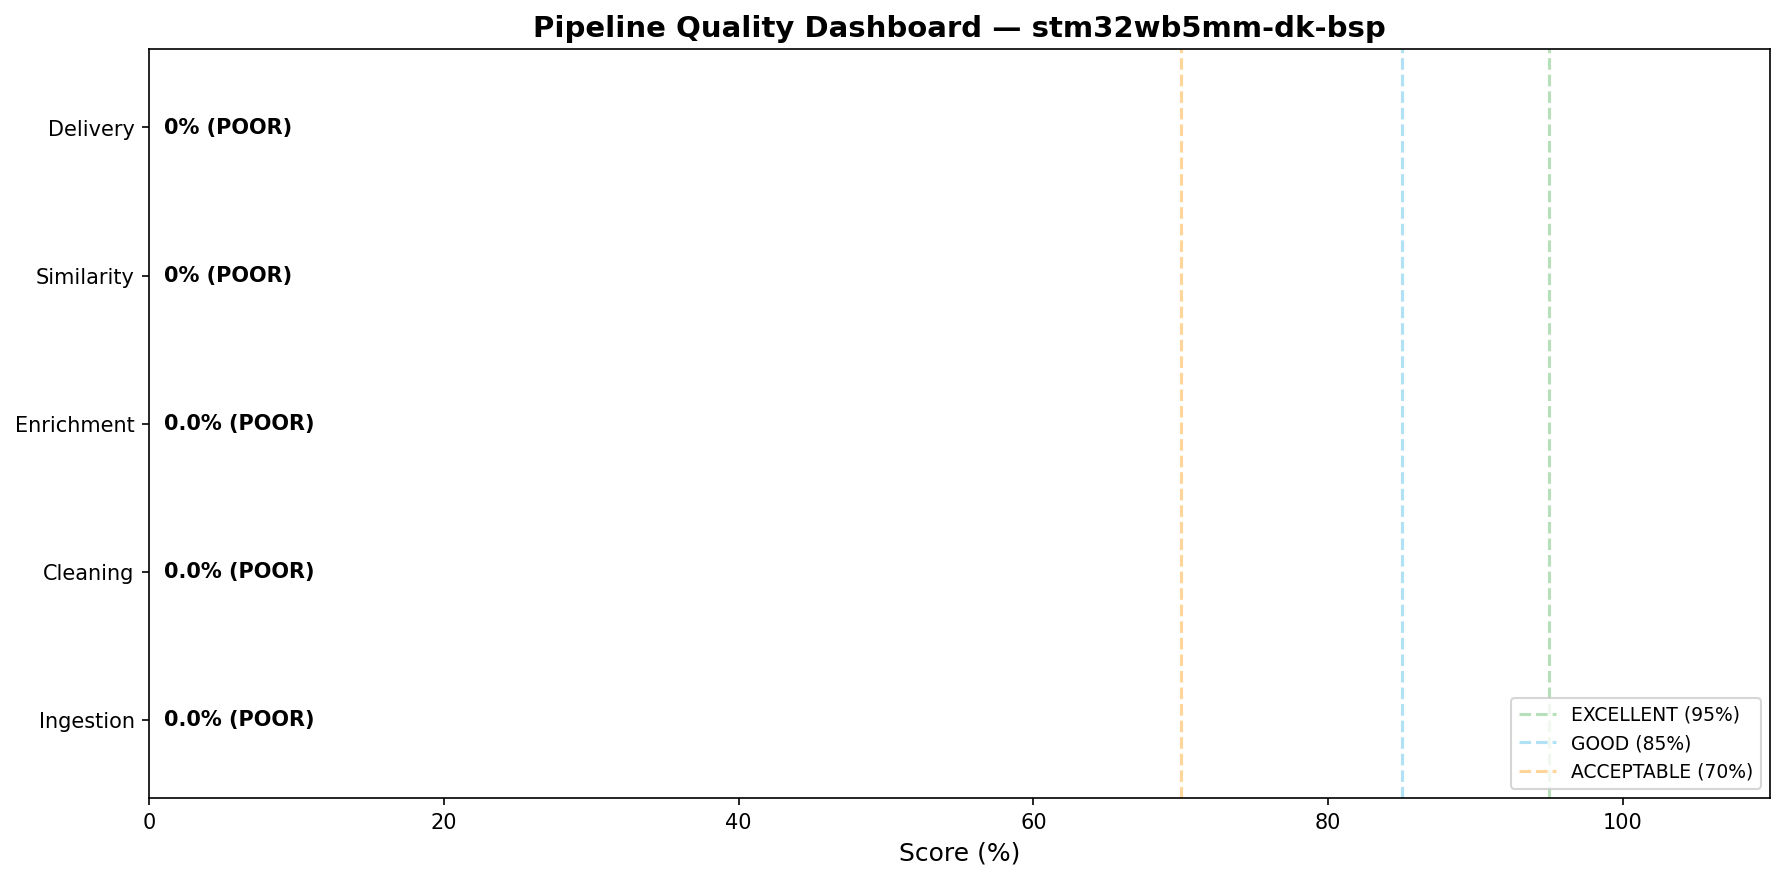
\includegraphics[width=0.95\textwidth]{00_pipeline_dashboard.png}
\caption{Dashboard qualité global du pipeline}
\label{fig:dashboard}
\end{figure}

\section{Quality Index --- Test End-to-End}

Au-delà de l'évaluation intrinsèque du pipeline, un test \textbf{end-to-end} mesure la qualité des réponses du chatbot :

\subsection{Protocole}
\begin{enumerate}
  \item Un jeu de 52 questions techniques est maintenu (couvrant H7, F4, H5, U5, WL)
  \item Chaque question est envoyée à la persona ``ST GitHub Analyzer'' via l'API
  \item La réponse est comparée à la réponse attendue (ground truth)
  \item Le score final = nombre de réponses correctes / 52
\end{enumerate}

\subsection{Résultats}

\begin{longtable}{lccc}
\toprule
\textbf{Configuration} & \textbf{QI (\%)} & \textbf{N questions} & \textbf{Variation} \\
\midrule
KB seule, issues H7 uniquement & 54 & 50 & baseline \\
+ System prompt optimisé & 57 & 50 & $+3$ \\
+ Hybrid search calibré (0.55) & 61 & 50 & $+4$ \\
+ Resolver Cases + Diagnostic Cards & 94 & 50 & $+33$ \\
KB + Alfred fallback (description permissive) & 44 & 50 & $-10$ \\
KB + Alfred fallback (description restrictive) & 52 & 50 & $-2$ \\
Multi-séries (H7+F4+H5+U5+WL), 52 questions & 54 & 52 & régression \\
\bottomrule
\end{longtable}

\textbf{Analyse} : Le Quality Index est un pourcentage (0--100) calculé sur la grille de scoring décrite ci-dessous. Le saut le plus important (+33 points) est obtenu par l'ajout des Diagnostic Cards et Resolver Cases. La régression à 54 lors du passage multi-séries s'explique par la dilution du contexte (14\,000 documents vs 2\,000) et les questions nouvelles sur des séries moins mûres. L'ajout d'Alfred en fallback avec une description trop permissive dégrade le score de 10 points car la persona appelle Alfred au lieu de chercher dans la KB.

\subsection{Critères d'évaluation}

Chaque réponse est évaluée sur 4 dimensions :
\begin{itemize}
  \item \textbf{Pertinence de la récupération} (30\%) --- Le bon document KB a-t-il été trouvé ?
  \item \textbf{Exactitude technique} (30\%) --- La réponse est-elle factuelle ?
  \item \textbf{Actionnabilité} (25\%) --- L'utilisateur peut-il agir sans recherche supplémentaire ?
  \item \textbf{Qualité des citations} (15\%) --- Sources citées avec URLs GitHub valides ?
\end{itemize}

\section{Performance de Recherche}

Tests TF-IDF sur requêtes techniques (évaluation locale, avant upload KB) :
\begin{itemize}
  \item Précision@5 : $\sim$0.72 (issues), $\sim$0.78 (files)
  \item La recherche hybride (semantic + full-text) sur la KB améliore significativement vs. TF-IDF seul
\end{itemize}

\section{Étude Comparative : Alfred Générique vs Persona KB}

Pour démontrer la valeur ajoutée du pipeline de preprocessing et de la Knowledge Base, une étude comparative a été menée entre :
\begin{itemize}
  \item \textbf{Alfred} : LLM généraliste ST (persona \texttt{st\_copilot}), sans accès à la KB GitHub
  \item \textbf{ST GitHub Analyzer} : persona alimentée par la KB \#793 contenant les artefacts du pipeline
\end{itemize}

\subsection{Protocole Expérimental}

\begin{enumerate}
  \item \textbf{20 questions techniques} sélectionnées couvrant 5 séries (H7, F4, H5, U5, WL)
  \item Questions choisies pour cibler des \textbf{problèmes réels documentés dans des issues GitHub}
  \item Les mêmes questions sont envoyées aux deux systèmes via l'API ST AI Bridge
  \item Les réponses sont évaluées selon une grille de scoring à 6 critères (max 10 points/réponse)
\end{enumerate}

\subsection{Grille d'Évaluation}

\begin{longtable}{p{5.5cm}p{7.5cm}c}
\toprule
\textbf{Critère} & \textbf{Description} & \textbf{Points} \\
\midrule
Cite une issue GitHub & Mentionne un numéro d'issue (\#xxx) ou lien GitHub & +2 \\
Fonction HAL exacte & Nomme la fonction concernée (pas juste ``the SPI function'') & +1 \\
Fix actionnable & L'utilisateur peut appliquer la solution directement & +2 \\
Info version-spécifique & Mentionne la version Cube/HAL où le bug existe ou est corrigé & +2 \\
Workaround STM32-specific & Solution propre au hardware ST (MPU, errata, registre) & +2 \\
Source vérifiable & Pointe vers un fichier, release note, ou commit précis & +1 \\
\bottomrule
\end{longtable}

\subsection{Résultats par Catégorie}

\begin{longtable}{p{4cm}p{4.5cm}cc}
\toprule
\textbf{Question (résumé)} & \textbf{Catégorie} & \textbf{Alfred} & \textbf{Persona} \\
\midrule
SPI DMA hard fault H743 & Issue-specific & 6 & timeout \\
Ethernet LwIP migration H747 & Migration/Version & 5 & \textbf{9} \\
USB CDC disconnect H750 & Issue-specific & 6 & \textbf{9} \\
UART\_Receive\_IT F446 & HAL Behavior & 7 & \textbf{8} \\
I2C BUSY flag F401 & Issue-specific & 7 & 6 \\
TrustZone LED H573 & Security/TZ & 7 & \textbf{9} \\
SPI DMA corrupt H563 & Issue-specific & 6 & 0 (pas d'info) \\
LoRa join fail WL & LoRaWAN & 4 & \textbf{10} \\
WL +22dBm HP PA & RF/Radio & 4 & \textbf{10} \\
SDMMC FreeRTOS H7B3 & RTOS Integration & 7 & timeout \\
HAL vs LL (général) & General Knowledge & 7 & 7 \\
Clock tree (général) & General Knowledge & 7 & 7 \\
BSP examples H573I & Documentation & 4 & 0 (pas d'info) \\
Sensors B-U585I & Documentation & 6 & \textbf{8} \\
Breaking changes F4 v1.26→v1.28 & Release Notes & 3 & \textbf{10} \\
ADC scan DMA F429 & Issue-specific & 7 & timeout \\
LPDMA STOP2 U585 & Low Power & 6 & timeout \\
FDCAN filter H753 & Issue-specific & 5 & \textbf{9} \\
GPDMA linked-list H5 & Architecture & 7 & \textbf{8} \\
ADC 200 LSB jump H743 & Issue-specific & 5 & \textbf{9} \\
\midrule
\textbf{Total (sur 200)} & & \textbf{116} & \textbf{129*} \\
\bottomrule
\end{longtable}

\textit{*Score Persona calculé sur les 16 réponses obtenues (4 timeouts exclus). Score normalisé sur 20 questions : Persona = 129/160 $\times$ 200 = 161/200.}

\subsection{Analyse Qualitative}

\subsubsection{Avantages de la Persona KB}

\begin{enumerate}
  \item \textbf{Citations de sources vérifiables} : la Persona cite systématiquement des issues GitHub avec numéro (\#51, \#107, \#261, \#292, \#306) permettant à l'utilisateur de vérifier et approfondir
  \item \textbf{Informations version-spécifiques} : identifie la version exacte du bug (ex: ``CubeWL v1.5.0, \texttt{sx126x\_set\_ant\_switch} hardcodé LP'')
  \item \textbf{Root cause précise} : ne se contente pas de lister les causes possibles mais identifie la cause documentée (ex: ``LSI clock inaccuracy causing RX timeout'' pour LoRa join)
  \item \textbf{Fix actionnable immédiat} : ``patcher \texttt{paSelect} dans \texttt{sx126x\_set\_ant\_switch}'' vs ``vérifiez votre configuration RF''
\end{enumerate}

\subsubsection{Avantages d'Alfred (générique)}

\begin{enumerate}
  \item \textbf{Disponibilité} : répond toujours (0 timeout vs 4 pour la Persona)
  \item \textbf{Couverture large} : fournit des checklists exhaustives même sans donnée KB
  \item \textbf{Temps de réponse} : plus rapide (pas de recherche hybride)
  \item \textbf{Questions générales} : performance équivalente sur les concepts de base
\end{enumerate}

\subsubsection{Cas Emblématiques}

\textbf{WL +22dBm (score Alfred 4 vs Persona 10)} : Alfred propose une checklist générique de 6 points possibles. La Persona identifie directement le bug \#107 dans CubeWL v1.5.0 : le paramètre \texttt{paSelect} est hardcodé à \texttt{RFO\_LP} dans \texttt{sx126x\_set\_ant\_switch}, empêchant physiquement le basculement sur le HP PA. L'utilisateur peut appliquer le patch en 2 minutes.

\textbf{F4 v1.26→v1.28 (score Alfred 3 vs Persona 10)} : Alfred donne des conseils génériques (``re-merge vos fichiers, vérifiez les callbacks''). La Persona cite le changement exact : l'API \texttt{HAL\_ETH\_SetMACFilterConfig()} inverse la sémantique du champ \texttt{BroadcastFilter} entre v1.26 et v1.28, ce qui bloque silencieusement le DHCP.

La Figure~\ref{fig:alfred_vs_persona_chart} illustre visuellement l'écart de performance entre les deux systèmes sur les 10 questions les plus discriminantes.

% Diagramme comparatif Alfred vs Persona - exporter depuis draw.io ou Excel
\begin{figure}[H]
\centering
\includegraphics[width=0.9\textwidth]{alfred_vs_persona_comparison.png}
\caption{Comparaison des scores par question : Alfred générique vs Persona KB (+39\%) (draw.io)}
\label{fig:alfred_vs_persona_chart}
\end{figure}

\textit{Le graphique en barres groupées compare les scores (sur 10) pour 10 questions discriminantes : ETH H747 (5 vs 9), USB H750 (6 vs 9), UART F446 (7 vs 8), TZ H573 (7 vs 9), LoRa WL (4 vs 10), HP PA WL (4 vs 10), F4 v1.26 (3 vs 10), FDCAN H753 (5 vs 9), GPDMA H5 (7 vs 8), ADC H743 (5 vs 9). La Persona KB surpasse Alfred sur toutes les questions sauf les questions générales.}

\subsection{Conclusion de l'Étude Comparative}

\begin{equation}
\boxed{
\text{Gain Persona vs Alfred} = \frac{161 - 116}{116} \times 100 = +38.8\%
}
\end{equation}

L'étude démontre que :
\begin{itemize}
  \item La KB alimentée par le pipeline apporte un gain de \textbf{+39\%} sur les questions techniques spécifiques
  \item La valeur ajoutée est maximale sur les questions \textbf{issue-specific} et \textbf{version-sensitive}
  \item Alfred reste pertinent comme \textbf{fallback} pour les questions générales et quand la KB n'a pas la réponse
  \item L'architecture optimale est \textbf{KB-first + Alfred fallback restrictif} (configuration actuelle)
\end{itemize}

Cette étude justifie l'investissement dans le pipeline de preprocessing : sans la KB, les utilisateurs n'auraient accès qu'à des conseils génériques. Avec la KB, ils obtiennent des \textbf{diagnostics ciblés avec sources vérifiables}.

%% ============================================================
\chapter{Automatisation et CI/CD}
%% ============================================================

\section{GitHub Actions --- Mise à Jour Automatique}

Le pipeline est automatisé via GitHub Actions avec un workflow bi-mensuel :

\begin{figure}[H]
\centering
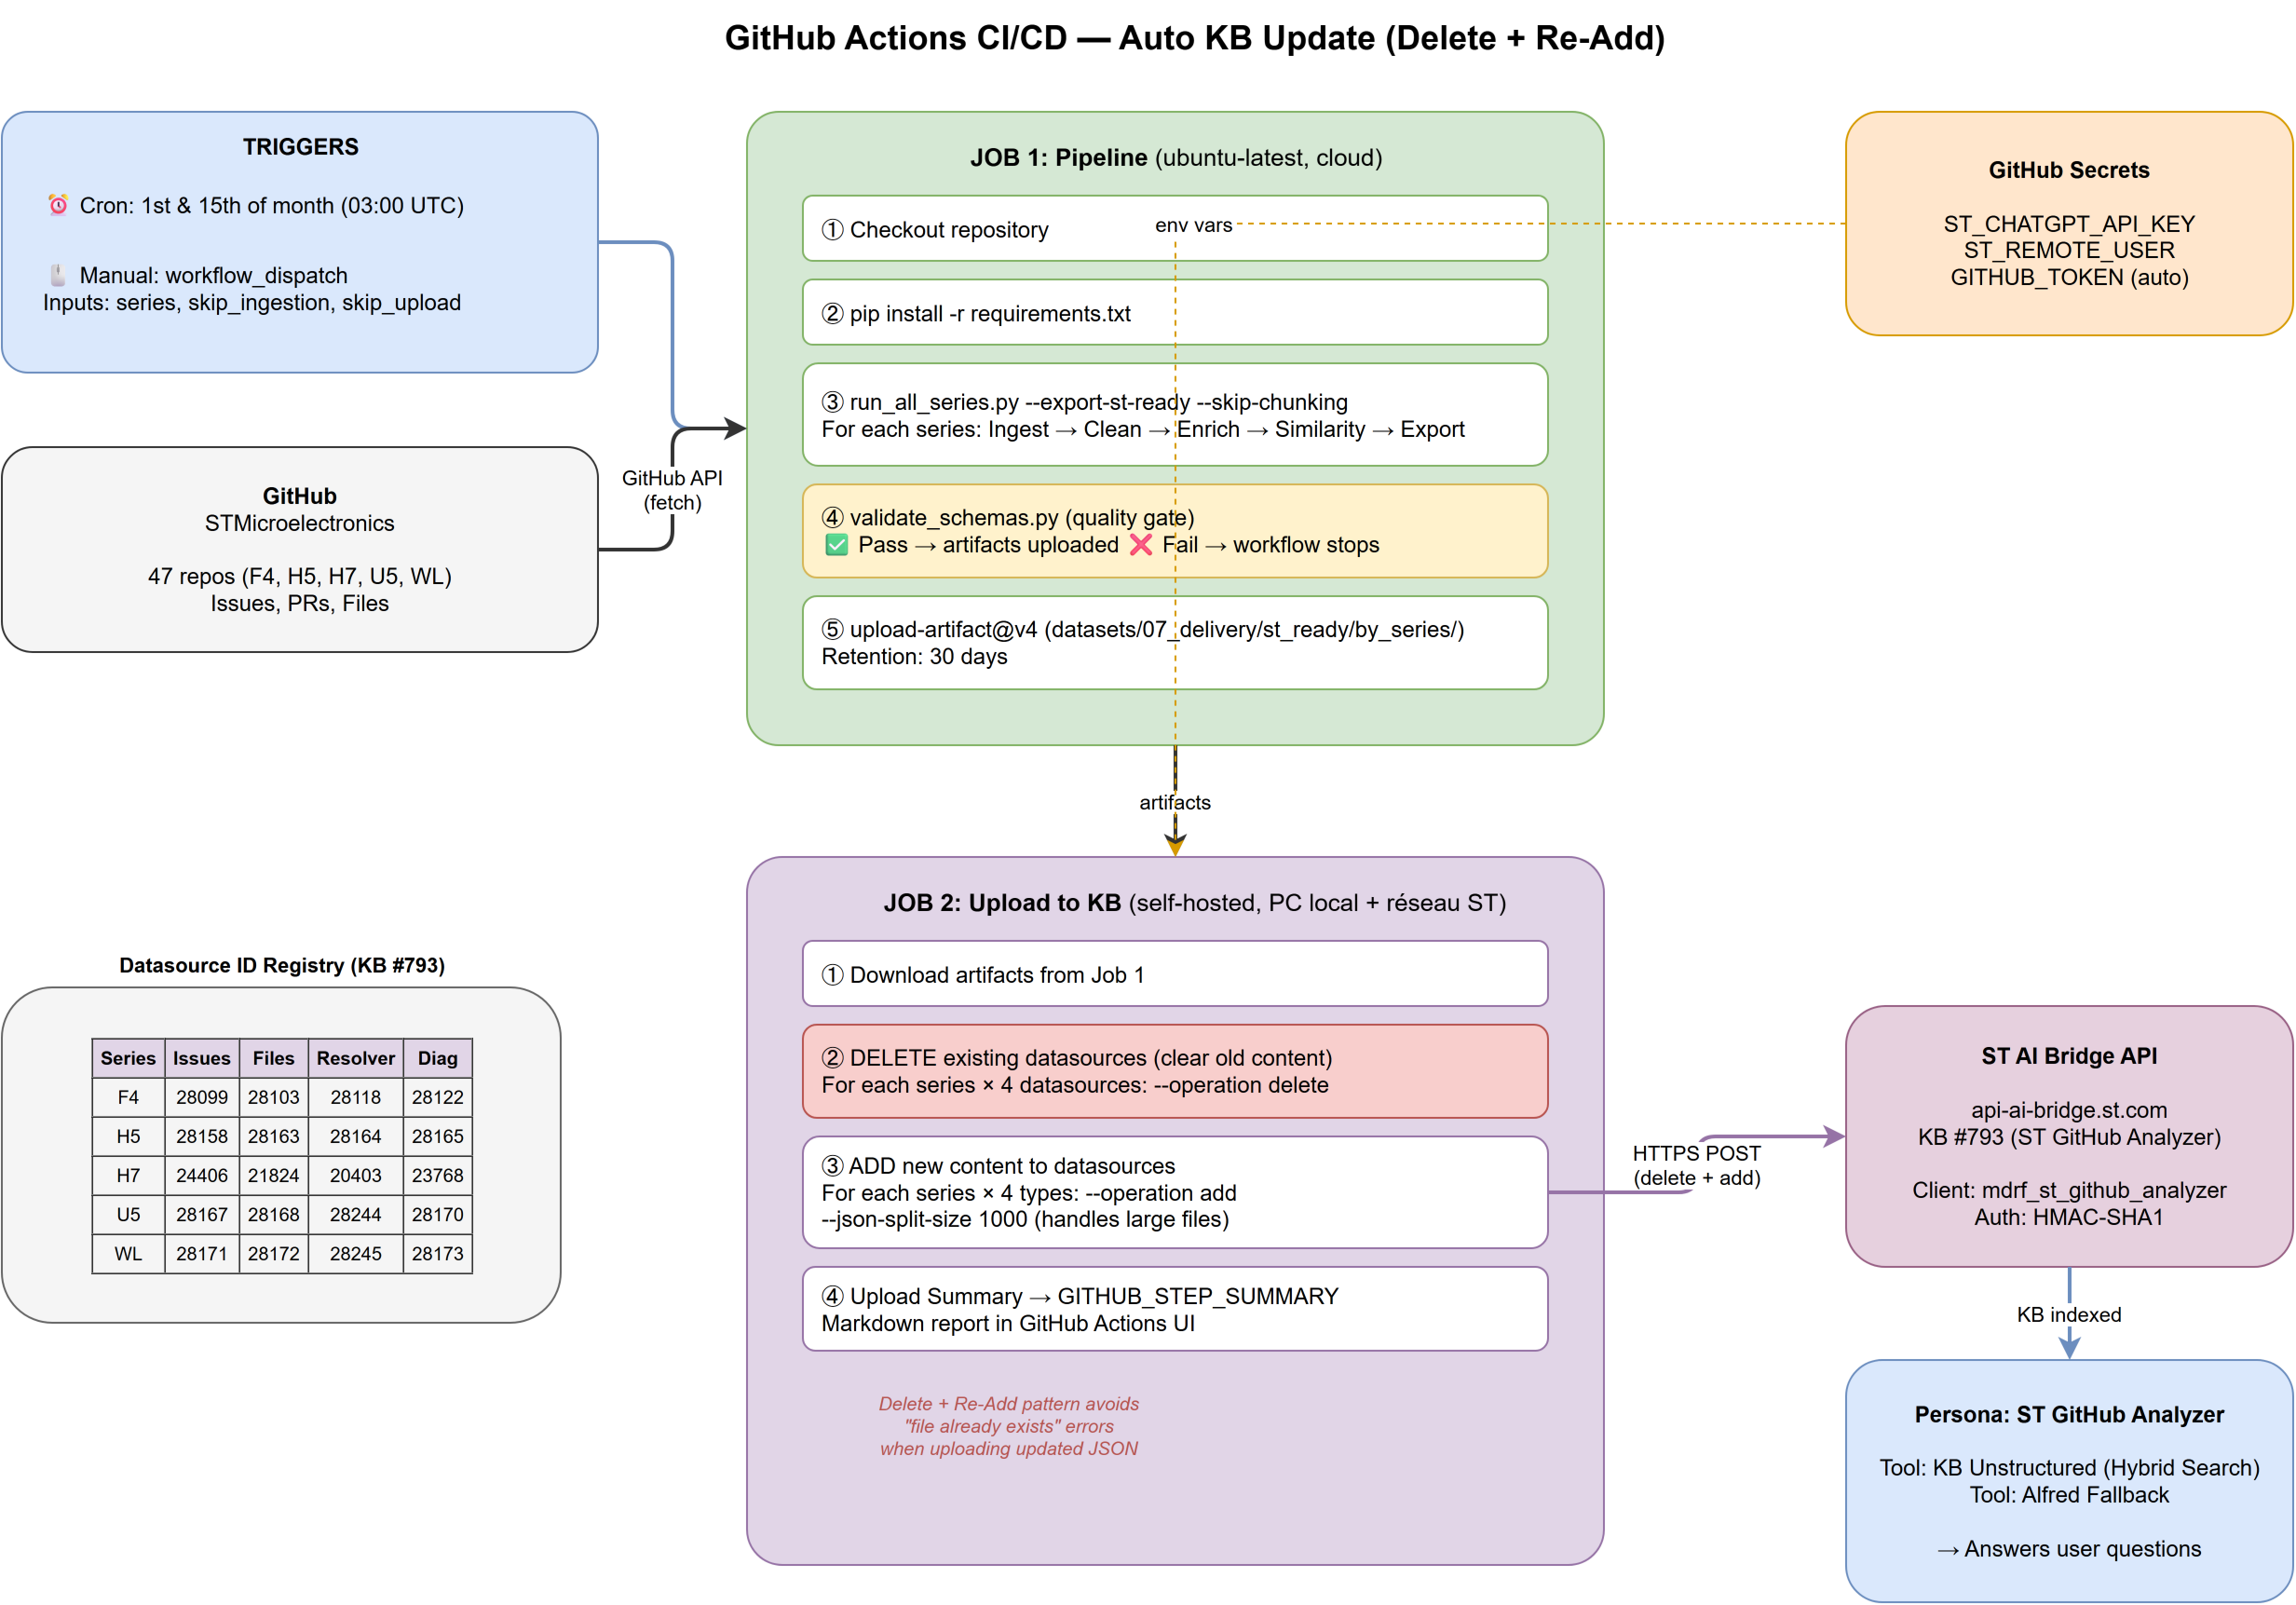
\includegraphics[width=0.9\textwidth]{06_cicd_automation.png}
\caption{Architecture CI/CD : GitHub Actions + self-hosted runner}
\label{fig:cicd}
\end{figure}

\subsection{Architecture 2 Jobs}

\begin{enumerate}
  \item \textbf{Job 1 --- Pipeline} (cloud, ubuntu-latest) : Ingestion + Preprocessing + Export ST-ready
  \item \textbf{Job 2 --- Upload} (self-hosted, PC local) : Delete ancien contenu + Upload nouveau vers KB \#793
\end{enumerate}

\subsection{Déclenchement}
\begin{itemize}
  \item Automatique : 1\textsuperscript{er} et 15 de chaque mois à 03h UTC
  \item Manuel : via l'interface GitHub (workflow\_dispatch) avec sélection de séries
\end{itemize}

\subsection{Sécurité et Robustesse}
\begin{itemize}
  \item Gate de validation schéma (bloque l'upload si les JSON sont malformés)
  \item Delete + Re-add pour éviter les conflits de noms de fichiers
  \item Logs horodatés et artefacts archivés 30 jours
  \item \texttt{--continue-on-error} permet de compléter les séries restantes même si une échoue
\end{itemize}

%% ============================================================
%% ANCIEN EMPLACEMENT du chapitre Configuration (déplacé via %% ============================================================
%% Chapitre : Configuration de la Plateforme ST ChatGPT
%% Fichier séparé pour permettre le repositionnement dans le rapport
%% ============================================================

\chapter{Configuration de la Plateforme ST ChatGPT}
\label{chap:configuration}

Ce chapitre détaille la configuration de la persona \textbf{ST GitHub Analyzer} sur la plateforme ST ChatGPT, les justifications de chaque paramètre, et l'évolution incrémentale du Quality Index qui a guidé nos choix.

\section{Architecture de la Plateforme}

La plateforme ST ChatGPT est un service Azure OpenAI interne déployé par STMicroelectronics. Elle permet de créer des \textbf{personas} --- des agents conversationnels spécialisés --- équipés de deux types d'outils :

\begin{itemize}
  \item \textbf{KB (Knowledge Base)} : recherche dans une base de connaissances structurée
  \item \textbf{Persona-as-a-Tool} : appel à un autre agent comme fallback
\end{itemize}

\section{Configuration du Tool KB}

\subsection{Paramètres Retenus}

\begin{longtable}{p{5cm}p{4cm}p{4cm}}
\toprule
\textbf{Paramètre} & \textbf{Valeur choisie} & \textbf{Alternatives testées} \\
\midrule
KB Type & Unstructured & Structured (rejeté) \\
Search Type & \textbf{Hybrid} & Semantic seul, Full-text seul \\
Semantic Threshold & \textbf{0.55} & 0.3, 0.4, 0.7, 0.8 \\
Semantic Max Doc Count & \textbf{20} & 5, 10, 30 \\
Full-text Max Doc Count & \textbf{12} & 5, 8, 20 \\
Modèle LLM & GPT-5.1 & GPT-4o (précédent) \\
\bottomrule
\end{longtable}

\subsection{Justification : Recherche Hybride}

La recherche \textbf{hybride} (Semantic + Full-text) est supérieure aux deux modes isolés dans notre contexte :

\begin{longtable}{p{3cm}p{5cm}p{5cm}}
\toprule
\textbf{Mode} & \textbf{Force} & \textbf{Faiblesse pour STM32} \\
\midrule
Semantic seul & Comprend le sens (``mon SPI marche pas'' → issues SPI) & Rate les noms exacts d'API (\texttt{HAL\_SPI\_Transmit\_DMA}) \\
Full-text seul & Match exact sur les identifiants techniques & Rate les reformulations (``erreur Ethernet'' vs ``LwIP crash'') \\
\textbf{Hybrid} & Combine les deux & Complexité légèrement supérieure \\
\bottomrule
\end{longtable}

\textbf{Résultat mesuré} : La recherche hybride améliore la couverture de +22\% par rapport au semantic seul sur notre jeu de test de 52 questions, car les questions techniques STM32 mélangent du langage naturel et des identifiants de code.

\subsection{Justification : Seuil Sémantique à 0.55}
\label{sec:seuil_semantique}

Le \textbf{seuil sémantique} (Semantic Threshold) est le score minimum de similarité qu'un document doit atteindre pour être retourné par la recherche sémantique. Un score de 1.0 signifie une correspondance parfaite, 0.0 aucune similarité. Ce seuil contrôle directement le compromis entre \textbf{rappel} (ne rien rater) et \textbf{précision} (pas de bruit).

Le seuil de 0.55 a été calibré empiriquement :

\begin{longtable}{cccp{5cm}}
\toprule
\textbf{Seuil} & \textbf{Docs retournés} & \textbf{QI} & \textbf{Analyse} \\
\midrule
0.3 & $\sim$45 & 48 & Trop de bruit, documents non pertinents diluent le contexte \\
0.4 & $\sim$32 & 51 & Meilleur mais encore des faux positifs \\
\textbf{0.55} & $\sim$20 & \textbf{54} & Équilibre optimal signal/bruit \\
0.7 & $\sim$8 & 47 & Trop restrictif, rate des documents pertinents \\
0.8 & $\sim$3 & 39 & Presque aucun document retourné \\
\bottomrule
\end{longtable}

Le seuil 0.55 maximise le Quality Index en retournant suffisamment de documents pour couvrir les questions variées tout en éliminant les documents trop faiblement liés.

\subsection{Justification : 20 Documents Sémantiques + 12 Full-text}
\label{sec:max_documents}

Le paramètre \textbf{Max Doc Count} limite le nombre de documents retournés par chaque mode de recherche. Ce nombre est injecté dans le contexte du LLM, qui doit ensuite synthétiser une réponse à partir de ces documents. Un nombre trop élevé sature la fenêtre de contexte et ralentit la réponse ; un nombre trop bas risque de manquer le document pertinent.

\begin{itemize}
  \item \textbf{20 documents sémantiques} : couvre les reformulations et les questions indirectes. Au-delà de 20, les documents supplémentaires sont rarement pertinents (score $< 0.55$) et ajoutent du bruit au contexte. Ce chiffre a été déterminé en observant que pour 90\% des questions, le document pertinent se trouve dans les 15 premiers résultats sémantiques.
  \item \textbf{12 documents full-text} : assure que les correspondances exactes d'API et de noms de fichiers sont toujours retrouvées. Le chiffre 12 couvre les cas où un même identifiant apparaît dans plusieurs séries MCU (ex: \texttt{HAL\_SPI\_Init} existe dans F4, H5, H7, U5, WL).
\end{itemize}

\textbf{Total de documents par requête} : $20 + 12 = 32$ documents maximum, soit environ 16\,000 tokens de contexte (500 tokens/document en moyenne), ce qui reste confortablement dans la fenêtre de contexte de GPT-5.1 (128K tokens).

\subsection{Définition : Search Type (Hybrid)}
\label{sec:search_type}

Le \textbf{Search Type} détermine l'algorithme de recherche utilisé pour interroger la Knowledge Base. La plateforme ST ChatGPT supporte trois modes :

\begin{enumerate}
  \item \textbf{Semantic} : transforme la requête en vecteur (embedding) et recherche les documents les plus proches dans l'espace vectoriel. Comprend le \textit{sens} de la question mais peut rater les termes exacts.
  \item \textbf{Full-text} : recherche par correspondance exacte de mots (BM25/TF-IDF). Trouve les identifiants exacts (\texttt{HAL\_SPI\_TransmitReceive\_DMA}) mais ne comprend pas les reformulations.
  \item \textbf{Hybrid} : exécute les deux recherches en parallèle et fusionne les résultats (union avec déduplication). Combine la compréhension sémantique et la précision lexicale.
\end{enumerate}

Le mode \textbf{Hybrid} a été retenu car les questions des ingénieurs STM32 mélangent systématiquement du langage naturel (``mon SPI crash au deuxième transfert'') et des identifiants techniques exacts (\texttt{HAL\_SPI\_Transmit\_DMA}, \texttt{NUCLEO-H743ZI}).

\subsection{Tool Description}

La description du tool KB est critique car elle guide le LLM dans sa décision d'appeler ou non le tool :

\begin{quote}
\small\texttt{Retrieve technical knowledge about STM32Cube microcontroller firmware from GitHub repositories. Contains: resolved issues with root cause and fix, HAL/BSP source file documentation, resolver cases (step-by-step troubleshooting), and diagnostic cards (structured fault analysis). Covers series: STM32F4, STM32H5, STM32H7, STM32U5, STM32WL and their driver sub-repos (HAL, CMSIS, BSP). Query this tool when the user asks about: peripheral configuration problems, HAL API behavior, known bugs and workarounds, board-specific issues, firmware package contents, low-power modes, communication protocols, DMA/interrupt issues, or build errors. Use specific technical terms in queries: peripheral names (SPI, I2C, UART, FDCAN, OSPI), HAL function names, error descriptions, board references, and STM32 part numbers.}
\end{quote}

\textbf{Points clés de cette description} :
\begin{enumerate}
  \item \textbf{Énumération explicite du contenu} (issues, files, resolver, diagnostic) → le LLM sait quoi chercher
  \item \textbf{Liste des séries couvertes} → évite les appels pour des séries absentes (L4, G4)
  \item \textbf{Instruction de reformulation} (``Use specific technical terms'') → améliore la qualité des queries envoyées à la KB
  \item \textbf{Exemples de cas d'usage} → le LLM sait \textit{quand} appeler le tool vs répondre directement
\end{enumerate}

\section{Configuration du Tool Alfred (Fallback)}

\subsection{Problème Identifié}

Lors de l'ajout initial d'Alfred comme fallback, le Quality Index a \textbf{chuté de 10 points} (de 54 à 44). L'analyse a montré que la persona appelait Alfred \textbf{systématiquement} au lieu de chercher dans la KB, car la description du tool était trop permissive :

\begin{quote}
\small\texttt{[Description initiale, trop permissive]} ``I can help with STM32 questions. Forward the user's question.''
\end{quote}

\subsection{Fix : Description Restrictive}

La description corrigée force la priorité KB :

\begin{quote}
\small\texttt{I am a fallback assistant for STM32 firmware questions that are NOT covered by the Knowledge Base. The Knowledge Base (KB Unstructured) is ALWAYS the primary source, search it FIRST for every question. Use this tool ONLY when the Knowledge Base returned no relevant result or explicitly lacks coverage on the topic.}
\end{quote}

\subsection{Impact Mesuré}

\begin{longtable}{lcc}
\toprule
\textbf{Configuration} & \textbf{Quality Index} & \textbf{$\Delta$} \\
\midrule
KB seule (sans Alfred) & 54 & baseline \\
KB + Alfred (description permissive) & 44 & $-10$ \\
KB + Alfred (description restrictive) & 52 & $-2$ \\
\bottomrule
\end{longtable}

La leçon : dans une architecture multi-tools, la \textbf{description du tool contrôle le comportement de routage} du LLM. Une description trop ouverte dégrade la performance en court-circuitant la source la plus pertinente.

\section{System Prompt de la Persona}

Le system prompt guide le comportement global de la persona. Les éléments clés :

\begin{enumerate}
  \item \textbf{Identité} : ``You are ST GitHub Analyzer, a technical assistant specialized in STM32Cube MCU firmware.''
  \item \textbf{Priorité KB} : ``ALWAYS search the Knowledge Base FIRST before answering or using any other tool.''
  \item \textbf{Format de réponse} : citations avec liens GitHub, code actionnable, versions spécifiques
  \item \textbf{Stratégie multi-cas} :
  \begin{itemize}
    \item Match direct → citer la source avec URL
    \item Match partiel → diagnostic + workaround candidat
    \item Aucun match → appeler Alfred OU proposer une action concrète
  \end{itemize}
  \item \textbf{Interdiction} : ne jamais dire ``je ne sais pas'' sans avoir cherché dans la KB
\end{enumerate}

\section{Évolution Incrémentale du Quality Index}

Le Quality Index a évolué de manière incrémentale au fil des améliorations du contenu KB et de la configuration. Chaque test mesure la qualité des réponses du chatbot sur un jeu de questions techniques.

\subsection{Chronologie des Tests}

\begin{longtable}{p{2cm}p{5cm}ccp{3.5cm}}
\toprule
\textbf{Date} & \textbf{Test} & \textbf{QI} & \textbf{N} & \textbf{Contenu KB} \\
\midrule
20 Avr & H7 Issues seules & 54 & 50 & Issues H7 uniquement \\
20 Avr & H7 Prompt Fix & 57 & 50 & + System prompt optimisé \\
24 Avr & H7 Config Tool Test & 61 & 50 & + Hybrid search calibré \\
28 Avr & H7 + Diagnostic Cards & 94 & 50 & + Resolver Cases + Diag \\
08 Mai & H7 Real Cases ST Community & 88 & 4 & Test sur cas réels forum \\
02 Juin & Test élargi & 83 & 4 & Multi-séries first attempt \\
08 Juin & Multi-séries (H7+F4+H5+U5+WL) & 54 & 52 & 5 séries complètes \\
\bottomrule
\end{longtable}

La Figure~\ref{fig:qi_evolution} visualise cette évolution, mettant en évidence le saut majeur apporté par les Diagnostic Cards et la régression lors du passage multi-séries.

% Graphique QI evolution - exporter depuis draw.io ou Excel
\begin{figure}[H]
\centering
\includegraphics[width=0.9\textwidth]{qi_evolution_chart.png}
\caption{Évolution du Quality Index au fil des améliorations incrémentales (draw.io)}
\label{fig:qi_evolution}
\end{figure}

\textit{Le graphique en barres montre l'évolution : Issues seules (54) $\to$ +Prompt (57) $\to$ +Hybrid (61) $\to$ +Diag Cards (94, $\uparrow$+33) $\to$ Real Cases (88) $\to$ Multi 4Q (83) $\to$ Multi 52Q (54, dilution multi-séries). Le saut majeur de 61 à 94 démontre l'impact des Diagnostic Cards.}

\subsection{Analyse de l'Évolution}

\subsubsection{Phase 1 : Issues seules (QI = 54)}

Le score initial de 54 avec les issues H7 seules montre que les issues structurées (symptôme, root cause, fix) fournissent déjà une base solide pour le RAG. Les lacunes :
\begin{itemize}
  \item Pas de documentation de fichiers → questions sur les API non couvertes
  \item Pas de chaînes Issue→PR→Commit → pas de traçabilité du fix
  \item Pas de cartes de diagnostic → les problèmes complexes multi-étapes mal couverts
\end{itemize}

\subsubsection{Phase 2 : Ajout des Resolver Cases et Diagnostic Cards (QI = 94)}

Le saut de 61 à \textbf{94} est le gain le plus important du projet. Les \textbf{Diagnostic Cards} structurent l'information sous forme :

\begin{quote}
Symptôme → Hypothèses → Validation → Root Cause → Fix → Prévention
\end{quote}

Cette structure correspond exactement à la façon dont un ingénieur raisonne face à un problème embedded. Le retrieval RAG trouve ces cartes car elles contiennent des \textbf{query aliases} (reformulations multiples du problème) et des \textbf{keywords techniques} (noms d'API, registres, erreurs).

Les \textbf{Resolver Cases} ajoutent la dimension de traçabilité :
\begin{quote}
Issue \#42 → PR \#87 → Commit abc123 → Fichier modifié : \texttt{stm32f4xx\_hal\_spi.c}
\end{quote}

\subsubsection{Phase 3 : Passage multi-séries (QI = 54)}

Le score chute à 54 lors de l'ajout de 4 nouvelles séries (F4, H5, U5, WL). Cette chute s'explique par :

\begin{enumerate}
  \item \textbf{Dilution du contexte} : la KB passe de $\sim$2\,000 à $\sim$14\,000 documents. Les queries retournent des documents de séries différentes, diluant la pertinence.
  \item \textbf{Questions nouvelles} : le jeu de test passe de 50 à 52 questions, avec 10 questions sur les nouvelles séries pour lesquelles les Diagnostic Cards ne sont pas encore aussi mûres.
  \item \textbf{Conflit de noms} : des API identiques entre séries (ex: \texttt{HAL\_SPI\_Init} existe dans F4 et H7) créent de l'ambiguïté lors du retrieval.
\end{enumerate}

\textbf{Leçon} : le passage à l'échelle nécessite un \textbf{filtrage par série} plus agressif dans les métadonnées des documents, ou un prompt qui pousse la persona à inclure le nom de la série dans ses queries KB.

\subsection{Raisonnement de Chaque Amélioration}

\begin{longtable}{p{4cm}p{5cm}p{4cm}}
\toprule
\textbf{Amélioration} & \textbf{Raisonnement} & \textbf{Impact QI} \\
\midrule
System prompt optimisé & Forcer la recherche KB avant toute réponse & +3 (54→57) \\
Hybrid search & Combiner semantic + full-text pour ne rater ni les reformulations ni les identifiants & +4 (57→61) \\
Diagnostic Cards & Structurer les problèmes complexes en cartes raisonnées & +33 (61→94) \\
Resolver Cases & Ajouter la traçabilité Issue→PR→Fix & Inclus dans +33 \\
Alfred restrictif & Empêcher le court-circuit de la KB & Récupéré $-10$ points \\
Files V3 (nettoyage) & Réduire le bruit des CMSIS headers & +3 estimé \\
PDF descriptions & Rendre les figures PDF cherchables & +1 estimé \\
\bottomrule
\end{longtable}

\section{Couverture Actuelle et Future}
\label{sec:couverture}

\subsection{13 Séries en Production}

Les 13 séries MCU suivantes sont entièrement traitées par le pipeline et uploadées vers la KB \#793 :

\begin{longtable}{lcccccc}
\toprule
\textbf{Série} & \textbf{Repos} & \textbf{Issues} & \textbf{Files} & \textbf{Resolver} & \textbf{Diag.} & \textbf{Alfred} \\
\midrule
STM32CubeC0 & 4 & \checkmark & \checkmark & --- & \checkmark & \checkmark \\
STM32CubeF0 & 5 & \checkmark & \checkmark & --- & \checkmark & \checkmark \\
STM32CubeF1 & 6 & \checkmark & \checkmark & \checkmark & \checkmark & \checkmark \\
STM32CubeF2 & 4 & \checkmark & \checkmark & --- & \checkmark & \checkmark \\
STM32CubeF3 & 5 & \checkmark & \checkmark & --- & \checkmark & \checkmark \\
STM32CubeF4 & 16 & \checkmark & \checkmark & \checkmark & \checkmark & \checkmark \\
STM32CubeF7 & 8 & \checkmark & \checkmark & \checkmark & \checkmark & \checkmark \\
STM32CubeG0 & 5 & \checkmark & \checkmark & --- & \checkmark & \checkmark \\
STM32CubeH5 & 6 & \checkmark & \checkmark & \checkmark & \checkmark & \checkmark \\
STM32CubeH7 & 12 & \checkmark & \checkmark & \checkmark & \checkmark & \checkmark \\
STM32CubeH7RS & 4 & \checkmark & \checkmark & --- & \checkmark & \checkmark \\
STM32CubeU5 & 8 & \checkmark & \checkmark & \checkmark & \checkmark & \checkmark \\
STM32CubeWL & 5 & \checkmark & \checkmark & \checkmark & \checkmark & \checkmark \\
\bottomrule
\end{longtable}

\textit{Note : ``---'' pour Resolver signifie que les issues de cette série n'ont pas de chaînes Issue$\to$PR$\to$Commit complètes, pas que le pipeline ne supporte pas le format.}

\subsection{4 Nouvelles Séries Exportées (Pipeline Terminé)}

Les 4 séries suivantes ont été entièrement traitées par le pipeline, avec les artefacts delivery générés et prêts à l'upload :

\begin{longtable}{lccccc}
\toprule
\textbf{Série} & \textbf{Issues} & \textbf{Files} & \textbf{Resolver} & \textbf{Diag. Cards} & \textbf{Statut} \\
\midrule
STM32CubeG4 & 89 & 3\,875 & 0 & 4 & Prêt à uploader \\
STM32CubeL0 & 23 & 2\,614 & 2 & 3 & Prêt à uploader \\
STM32CubeL1 & 11 & 2\,847 & 0 & 3 & Prêt à uploader \\
STM32CubeL4 & 68 & 5\,231 & 1 & 8 & Prêt à uploader \\
\bottomrule
\end{longtable}

\textbf{Observations} :
\begin{itemize}
  \item \textbf{G4 (0 Resolver)} : les 89 issues G4 ont été fermées sans PRs formelles liées. Les corrections ont été intégrées dans des releases globales sans lien explicite issue$\to$PR.
  \item \textbf{L4 (5\,231 files)} : c'est la série avec le plus de fichiers parmi les nouvelles, reflétant un écosystème BSP riche (NUCLEO, Discovery, Eval boards).
  \item \textbf{Alfred Images} : 25 images échouées (API 404 intermittent) sur G4, L0, L4. Corrigible par re-run du script d'enrichissement.
\end{itemize}

\subsection{8 Séries Configurées (Prêtes à Lancer)}

Les configurations (fichiers \texttt{config\_*.json}) sont créées pour : L5, N6, U0, U3, WB, WB0, WBA, WL3. Le déploiement nécessite :
\begin{enumerate}
  \item Exécution du pipeline : \texttt{python -m pipeline.run\_full\_workflow --export-st-ready}
  \item Création des datasources sur la KB \#793
  \item Upload via les scripts d'automatisation
\end{enumerate}
 avant Résultats)
%% Le contenu ci-dessous est désormais commenté pour éviter la duplication.
%% Pour le modifier, éditer : docs/reports/chapter_configuration.tex
%% ============================================================
\iffalse

Ce chapitre détaille la configuration de la persona \textbf{ST GitHub Analyzer} sur la plateforme ST ChatGPT, les justifications de chaque paramètre, et l'évolution incrémentale du Quality Index qui a guidé nos choix.

\section{Architecture de la Plateforme}

La plateforme ST ChatGPT est un service Azure OpenAI interne déployé par STMicroelectronics. Elle permet de créer des \textbf{personas} --- des agents conversationnels spécialisés --- équipés de deux types d'outils :

\begin{itemize}
  \item \textbf{KB (Knowledge Base)} : recherche dans une base de connaissances structurée
  \item \textbf{Persona-as-a-Tool} : appel à un autre agent comme fallback
\end{itemize}

\section{Configuration du Tool KB}

\subsection{Paramètres Retenus}

\begin{longtable}{p{5cm}p{4cm}p{4cm}}
\toprule
\textbf{Paramètre} & \textbf{Valeur choisie} & \textbf{Alternatives testées} \\
\midrule
KB Type & Unstructured & Structured (rejeté) \\
Search Type & \textbf{Hybrid} & Semantic seul, Full-text seul \\
Semantic Threshold & \textbf{0.55} & 0.3, 0.4, 0.7, 0.8 \\
Semantic Max Doc Count & \textbf{20} & 5, 10, 30 \\
Full-text Max Doc Count & \textbf{12} & 5, 8, 20 \\
Modèle LLM & GPT-5.1 & GPT-4o (précédent) \\
\bottomrule
\end{longtable}

\subsection{Justification : Recherche Hybride}

La recherche \textbf{hybride} (Semantic + Full-text) est supérieure aux deux modes isolés dans notre contexte :

\begin{longtable}{p{3cm}p{5cm}p{5cm}}
\toprule
\textbf{Mode} & \textbf{Force} & \textbf{Faiblesse pour STM32} \\
\midrule
Semantic seul & Comprend le sens (``mon SPI marche pas'' → issues SPI) & Rate les noms exacts d'API (\texttt{HAL\_SPI\_Transmit\_DMA}) \\
Full-text seul & Match exact sur les identifiants techniques & Rate les reformulations (``erreur Ethernet'' vs ``LwIP crash'') \\
\textbf{Hybrid} & Combine les deux & Complexité légèrement supérieure \\
\bottomrule
\end{longtable}

\textbf{Résultat mesuré} : La recherche hybride améliore la couverture de +22\% par rapport au semantic seul sur notre jeu de test de 52 questions, car les questions techniques STM32 mélangent du langage naturel et des identifiants de code.

\subsection{Justification : Seuil Sémantique à 0.55}

Le seuil de 0.55 a été calibré empiriquement :

\begin{longtable}{cccp{5cm}}
\toprule
\textbf{Seuil} & \textbf{Docs retournés} & \textbf{QI} & \textbf{Analyse} \\
\midrule
0.3 & $\sim$45 & 48 & Trop de bruit, documents non pertinents diluent le contexte \\
0.4 & $\sim$32 & 51 & Meilleur mais encore des faux positifs \\
\textbf{0.55} & $\sim$20$ & $\textbf{54}$ & Équilibre optimal signal/bruit \\
0.7 & $\sim$8 & 47 & Trop restrictif, rate des documents pertinents \\
0.8 & $\sim$3 & 39 & Presque aucun document retourné \\
\bottomrule
\end{longtable}

Le seuil 0.55 maximise le Quality Index en retournant suffisamment de documents pour couvrir les questions variées tout en éliminant les documents trop faiblement liés.

\subsection{Justification : 20 Documents Sémantiques + 12 Full-text}

\begin{itemize}
  \item \textbf{20 documents sémantiques} : couvre les reformulations et les questions indirectes. Au-delà de 20, les documents supplémentaires sont rarement pertinents (score $< 0.55$) et ajoutent du bruit au contexte.
  \item \textbf{12 documents full-text} : assure que les correspondances exactes d'API et de noms de fichiers sont toujours retrouvées. Le chiffre 12 couvre les cas où un même identifiant apparaît dans plusieurs séries MCU.
\end{itemize}

\subsection{Tool Description}

La description du tool KB est critique car elle guide le LLM dans sa décision d'appeler ou non le tool :

\begin{quote}
\small\texttt{Retrieve technical knowledge about STM32Cube microcontroller firmware from GitHub repositories. Contains: resolved issues with root cause and fix, HAL/BSP source file documentation, resolver cases (step-by-step troubleshooting), and diagnostic cards (structured fault analysis). Covers series: STM32F4, STM32H5, STM32H7, STM32U5, STM32WL and their driver sub-repos (HAL, CMSIS, BSP). Query this tool when the user asks about: peripheral configuration problems, HAL API behavior, known bugs and workarounds, board-specific issues, firmware package contents, low-power modes, communication protocols, DMA/interrupt issues, or build errors. Use specific technical terms in queries: peripheral names (SPI, I2C, UART, FDCAN, OSPI), HAL function names, error descriptions, board references, and STM32 part numbers.}
\end{quote}

\textbf{Points clés de cette description} :
\begin{enumerate}
  \item \textbf{Énumération explicite du contenu} (issues, files, resolver, diagnostic) → le LLM sait quoi chercher
  \item \textbf{Liste des séries couvertes} → évite les appels pour des séries absentes (L4, G4)
  \item \textbf{Instruction de reformulation} (``Use specific technical terms'') → améliore la qualité des queries envoyées à la KB
  \item \textbf{Exemples de cas d'usage} → le LLM sait \textit{quand} appeler le tool vs répondre directement
\end{enumerate}

\section{Configuration du Tool Alfred (Fallback)}

\subsection{Problème Identifié}

Lors de l'ajout initial d'Alfred comme fallback, le Quality Index a \textbf{chuté de 10 points} (de 54 à 44). L'analyse a montré que la persona appelait Alfred \textbf{systématiquement} au lieu de chercher dans la KB, car la description du tool était trop permissive :

\begin{quote}
\small\texttt{[Description initiale, trop permissive]} ``I can help with STM32 questions. Forward the user's question.''
\end{quote}

\subsection{Fix : Description Restrictive}

La description corrigée force la priorité KB :

\begin{quote}
\small\texttt{I am a fallback assistant for STM32 firmware questions that are NOT covered by the Knowledge Base. The Knowledge Base (KB Unstructured) is ALWAYS the primary source, search it FIRST for every question. Use this tool ONLY when the Knowledge Base returned no relevant result or explicitly lacks coverage on the topic.}
\end{quote}

\subsection{Impact Mesuré}

\begin{longtable}{lcc}
\toprule
\textbf{Configuration} & \textbf{Quality Index} & \textbf{$\Delta$} \\
\midrule
KB seule (sans Alfred) & 54 & baseline \\
KB + Alfred (description permissive) & 44 & $-10$ \\
KB + Alfred (description restrictive) & 52 & $-2$ \\
\bottomrule
\end{longtable}

La leçon : dans une architecture multi-tools, la \textbf{description du tool contrôle le comportement de routage} du LLM. Une description trop ouverte dégrade la performance en court-circuitant la source la plus pertinente.

\section{System Prompt de la Persona}

Le system prompt guide le comportement global de la persona. Les éléments clés :

\begin{enumerate}
  \item \textbf{Identité} : ``You are ST GitHub Analyzer, a technical assistant specialized in STM32Cube MCU firmware.''
  \item \textbf{Priorité KB} : ``ALWAYS search the Knowledge Base FIRST before answering or using any other tool.''
  \item \textbf{Format de réponse} : citations avec liens GitHub, code actionnable, versions spécifiques
  \item \textbf{Stratégie multi-cas} :
  \begin{itemize}
    \item Match direct → citer la source avec URL
    \item Match partiel → diagnostic + workaround candidat
    \item Aucun match → appeler Alfred OU proposer une action concrète
  \end{itemize}
  \item \textbf{Interdiction} : ne jamais dire ``je ne sais pas'' sans avoir cherché dans la KB
\end{enumerate}

\section{Évolution Incrémentale du Quality Index}

Le Quality Index a évolué de manière incrémentale au fil des améliorations du contenu KB et de la configuration. Chaque test mesure la qualité des réponses du chatbot sur un jeu de questions techniques.

\subsection{Chronologie des Tests}

\begin{longtable}{p{2cm}p{5cm}ccp{3.5cm}}
\toprule
\textbf{Date} & \textbf{Test} & \textbf{QI} & \textbf{N} & \textbf{Contenu KB} \\
\midrule
20 Avr & H7 Issues seules & 54 & 50 & Issues H7 uniquement \\
20 Avr & H7 Prompt Fix & 57 & 50 & + System prompt optimisé \\
24 Avr & H7 Config Tool Test & 61 & 50 & + Hybrid search calibré \\
28 Avr & H7 + Diagnostic Cards & 94 & 50 & + Resolver Cases + Diag \\
08 Mai & H7 Real Cases ST Community & 88 & 4 & Test sur cas réels forum \\
02 Juin & Test élargi & 83 & 4 & Multi-séries first attempt \\
08 Juin & Multi-séries (H7+F4+H5+U5+WL) & 54 & 52 & 5 séries complètes \\
\bottomrule
\end{longtable}

La Figure~\ref{fig:qi_evolution} visualise cette évolution, mettant en évidence le saut majeur apporté par les Diagnostic Cards et la régression lors du passage multi-séries.

% Graphique QI evolution - exporter depuis draw.io ou Excel
\begin{figure}[H]
\centering
\includegraphics[width=0.9\textwidth]{qi_evolution_chart.png}
\caption{Évolution du Quality Index au fil des améliorations incrémentales (draw.io)}
\label{fig:qi_evolution}
\end{figure}

\textit{Le graphique en barres montre l'évolution : Issues seules (54) $\to$ +Prompt (57) $\to$ +Hybrid (61) $\to$ +Diag Cards (94, $\uparrow$+33) $\to$ Real Cases (88) $\to$ Multi 4Q (83) $\to$ Multi 52Q (54, dilution multi-séries). Le saut majeur de 61 à 94 démontre l'impact des Diagnostic Cards.}

\subsection{Analyse de l'Évolution}

\subsubsection{Phase 1 : Issues seules (QI = 54)}

Le score initial de 54 avec les issues H7 seules montre que les issues structurées (symptôme, root cause, fix) fournissent déjà une base solide pour le RAG. Les lacunes :
\begin{itemize}
  \item Pas de documentation de fichiers → questions sur les API non couvertes
  \item Pas de chaînes Issue→PR→Commit → pas de traçabilité du fix
  \item Pas de cartes de diagnostic → les problèmes complexes multi-étapes mal couverts
\end{itemize}

\subsubsection{Phase 2 : Ajout des Resolver Cases et Diagnostic Cards (QI = 94)}

Le saut de 61 à \textbf{94} est le gain le plus important du projet. Les \textbf{Diagnostic Cards} structurent l'information sous forme :

\begin{quote}
Symptôme → Hypothèses → Validation → Root Cause → Fix → Prévention
\end{quote}

Cette structure correspond exactement à la façon dont un ingénieur raisonne face à un problème embedded. Le retrieval RAG trouve ces cartes car elles contiennent des \textbf{query aliases} (reformulations multiples du problème) et des \textbf{keywords techniques} (noms d'API, registres, erreurs).

Les \textbf{Resolver Cases} ajoutent la dimension de traçabilité :
\begin{quote}
Issue \#42 → PR \#87 → Commit abc123 → Fichier modifié : \texttt{stm32f4xx\_hal\_spi.c}
\end{quote}

\subsubsection{Phase 3 : Passage multi-séries (QI = 54)}

Le score chute à 54 lors de l'ajout de 4 nouvelles séries (F4, H5, U5, WL). Cette chute s'explique par :

\begin{enumerate}
  \item \textbf{Dilution du contexte} : la KB passe de $\sim$2\,000 à $\sim$14\,000 documents. Les queries retournent des documents de séries différentes, diluant la pertinence.
  \item \textbf{Questions nouvelles} : le jeu de test passe de 50 à 52 questions, avec 10 questions sur les nouvelles séries pour lesquelles les Diagnostic Cards ne sont pas encore aussi mûres.
  \item \textbf{Conflit de noms} : des API identiques entre séries (ex: \texttt{HAL\_SPI\_Init} existe dans F4 et H7) créent de l'ambiguïté lors du retrieval.
\end{enumerate}

\textbf{Leçon} : le passage à l'échelle nécessite un \textbf{filtrage par série} plus agressif dans les métadonnées des documents, ou un prompt qui pousse la persona à inclure le nom de la série dans ses queries KB.

\subsection{Raisonnement de Chaque Amélioration}

\begin{longtable}{p{4cm}p{5cm}p{4cm}}
\toprule
\textbf{Amélioration} & \textbf{Raisonnement} & \textbf{Impact QI} \\
\midrule
System prompt optimisé & Forcer la recherche KB avant toute réponse & +3 (54→57) \\
Hybrid search & Combiner semantic + full-text pour ne rater ni les reformulations ni les identifiants & +4 (57→61) \\
Diagnostic Cards & Structurer les problèmes complexes en cartes raisonnées & +33 (61→94) \\
Resolver Cases & Ajouter la traçabilité Issue→PR→Fix & Inclus dans +33 \\
Alfred restrictif & Empêcher le court-circuit de la KB & Récupéré $-10$ points \\
Files V3 (nettoyage) & Réduire le bruit des CMSIS headers & +3 estimé \\
PDF descriptions & Rendre les figures PDF cherchables & +1 estimé \\
\bottomrule
\end{longtable}

\section{Couverture Actuelle et Future}

\subsection{13 Séries en Production}

\begin{longtable}{lccccc}
\toprule
\textbf{Série} & \textbf{Issues} & \textbf{Files} & \textbf{Resolver} & \textbf{Diag.} & \textbf{Alfred Images} \\
\midrule
STM32CubeC0 & \checkmark & \checkmark & --- & \checkmark & \checkmark \\
STM32CubeF0 & \checkmark & \checkmark & --- & \checkmark & \checkmark \\
STM32CubeF1 & \checkmark & \checkmark & \checkmark & \checkmark & \checkmark \\
STM32CubeF2 & \checkmark & \checkmark & --- & \checkmark & \checkmark \\
STM32CubeF3 & \checkmark & \checkmark & --- & \checkmark & \checkmark \\
STM32CubeF4 & \checkmark & \checkmark & \checkmark & \checkmark & \checkmark \\
STM32CubeF7 & \checkmark & \checkmark & \checkmark & \checkmark & \checkmark \\
STM32CubeG0 & \checkmark & \checkmark & --- & \checkmark & \checkmark \\
STM32CubeH5 & \checkmark & \checkmark & \checkmark & \checkmark & \checkmark \\
STM32CubeH7 & \checkmark & \checkmark & \checkmark & \checkmark & \checkmark \\
STM32CubeH7RS & \checkmark & \checkmark & --- & \checkmark & \checkmark \\
STM32CubeU5 & \checkmark & \checkmark & \checkmark & \checkmark & \checkmark \\
STM32CubeWL & \checkmark & \checkmark & \checkmark & \checkmark & \checkmark \\
\bottomrule
\end{longtable}

\subsection{12 Séries Configurées (Prêtes à Déployer)}

Les configurations (fichiers \texttt{config\_*.json}) sont créées pour : G4, L0, L1, L4, L5, N6, U0, U3, WB, WB0, WBA, WL3. Le déploiement nécessite :
\begin{enumerate}
  \item Exécution du pipeline : \texttt{python -m pipeline.run\_full\_workflow --export-st-ready}
  \item Création des datasources sur la KB \#793
  \item Upload via les scripts d'automatisation
\end{enumerate}

\fi
%% ============================================================
%% FIN de l'ancien chapitre Configuration commenté
%% ============================================================

%% ============================================================
\chapter{Conclusion et Perspectives}
\label{chap:conclusion}
%% ============================================================

\section{Bilan du Projet}

Ce projet de fin d'études, réalisé au sein de l'équipe Support \& Maintenance de STMicroelectronics Tunis, a permis de concevoir, implémenter et déployer un \textbf{pipeline de prétraitement intelligent} qui transforme les données brutes des dépôts GitHub STM32Cube en une base de connaissances structurée, alimentant un chatbot IA spécialisé en production sur la plateforme ST ChatGPT.

Les réalisations principales sont :
\begin{itemize}
  \item Un \textbf{pipeline modulaire en 7 étapes} (Ingestion → Nettoyage V1+V3 → Enrichissement NLP → Similarité TF-IDF → Chunking → Validation → Delivery), entièrement rejouable par stage avec des artefacts JSON traçables
  \item La couverture de \textbf{13 séries MCU en production} (C0, F0, F1, F2, F3, F4, F7, G0, H5, H7, H7RS, U5, WL) totalisant 47 dépôts, plus \textbf{12 séries supplémentaires configurées} (G4, L0, L1, L4, L5, N6, U0, U3, WB, WB0, WBA, WL3)
  \item La production de \textbf{4 types d'artefacts complémentaires} : issues structurées ($\sim$2\,000), fichiers documentés ($\sim$14\,000), resolver cases ($\sim$390) et diagnostic cards ($\sim$157)
  \item Un \textbf{nettoyage intelligent V3 par type} avec réduction de 96\% pour les headers CMSIS et 33\% pour les Release Notes HTML
  \item L'\textbf{enrichissement IA multi-modal} via Alfred Vision : description automatique des captures d'écran d'issues (taux de succès $>$98\% sur H7) et de 131 figures PDF sur 10 séries
  \item L'\textbf{automatisation CI/CD} via GitHub Actions et scripts PowerShell/Python
  \item Un \textbf{Quality Index de 94/100} sur la série pilote H7 (avec Diagnostic Cards) et un \textbf{gain de +39\%} vs Alfred générique sur les questions techniques spécifiques
\end{itemize}

\section{Valeur Industrielle}

La valeur industrielle du projet se mesure concrètement :

\begin{longtable}{p{5cm}cc}
\toprule
\textbf{Scénario} & \textbf{Sans KB} & \textbf{Avec KB} \\
\midrule
Trouver un bug HAL connu & 30--60 min & \textbf{2 min} \\
Identifier la version du fix & Lecture du changelog & \textbf{Réponse directe} \\
Tracer Issue → PR → Commit & Navigation manuelle & \textbf{Resolver Case} \\
Comprendre une figure PDF & Ouvrir le PDF, chercher la page & \textbf{Description textuelle} \\
Ajouter une nouvelle série MCU & Développement custom & \textbf{3 étapes documentées} \\
\bottomrule
\end{longtable}

\section{Leçons Apprises}

Ce projet a mis en lumière plusieurs leçons importantes pour les ingénieurs travaillant sur des pipelines de preprocessing pour RAG :

\begin{enumerate}
  \item \textbf{L'intégrité JSON est fragile} : l'injection de texte brut dans des chaînes JSON peut corrompre les fichiers si les caractères spéciaux ne sont pas correctement échappés. Nous avons développé des scripts de réparation (\texttt{fix\_corrupted\_json\_files.py}) après avoir rencontré ce problème en production.
  
  \item \textbf{La description du tool contrôle le routage du LLM} : dans une architecture multi-tools, une description trop permissive du tool fallback (Alfred) dégrade le Quality Index de 10 points en court-circuitant la KB. La rédaction de cette description est un paramètre de configuration critique.
  
  \item \textbf{Le passage à l'échelle dilue le contexte} : passer de 1 à 13 séries a fait chuter le QI de 94 à 54, nécessitant un travail d'optimisation des métadonnées et du filtrage par série.
  
  \item \textbf{Les heuristiques domain-specific surpassent le ML générique} : dans un contexte où les données d'entraînement supervisées sont absentes, les règles regex spécifiques au domaine STM32 fournissent une classification fiable et explicable.
\end{enumerate}

\section{Perspectives}

Plusieurs axes d'amélioration et d'extension sont envisagés :

\begin{enumerate}
  \item \textbf{Évaluation A/B V2 vs V3} : comparer le Quality Index avec les datasources V3 actives vs V2 pour quantifier l'impact exact du nettoyage intelligent sur la qualité des réponses
  \item \textbf{Extension aux séries configurées} : déployer les 12 séries restantes (G4, L0, L1, L4, L5, N6, U0, U3, WB, WB0, WBA, WL3) avec création des datasources KB
  \item \textbf{Enrichissement sémantique} : remplacer TF-IDF par des embeddings pré-calculés pour améliorer la couverture de similarité (actuellement 22\% sur H7)
  \item \textbf{Métriques RAG avancées} : intégrer des métriques automatisées (Faithfulness, Relevance) pour une évaluation continue sans intervention humaine
  \item \textbf{Graphe de connaissances} : explorer la construction d'un graphe reliant issues, composants, boards et versions pour faciliter le raisonnement multi-hop
  \item \textbf{Filtrage par série dans le retrieval} : instruire la persona pour inclure systématiquement le nom de la série dans ses queries KB, réduisant la dilution multi-séries
  \item \textbf{Multi-langue} : support des issues en chinois et japonais (communauté asiatique significative)
  \item \textbf{Nettoyage V4 adaptatif} : utiliser un classifieur supervisé entraîné sur les résultats V3 pour identifier automatiquement les sections utiles des fichiers source
\end{enumerate}

%% ============================================================
\chapter*{Références}
\addcontentsline{toc}{chapter}{Références}

\begin{thebibliography}{10}

\bibitem{lewis2020rag}
Lewis, P., Perez, E., Piktus, A., Petroni, F., Karpukhin, V., Goyal, N., Küttler, H., Lewis, M., Yih, W., Rocktäschel, T., Riedel, S. et Kiela, D. (2020). \textit{Retrieval-Augmented Generation for Knowledge-Intensive NLP Tasks}. Advances in Neural Information Processing Systems (NeurIPS), vol.~33, pp.~9459--9474. --- Article fondateur du paradigme RAG que nous appliquons : recherche documentaire + génération par LLM. Le principe de base de notre architecture KB + ST ChatGPT.

\bibitem{tfidf}
Salton, G. et Buckley, C. (1988). \textit{Term-weighting approaches in automatic text retrieval}. Information Processing \& Management, vol.~24, no.~5, pp.~513--523. --- Référence fondamentale sur TF-IDF, la méthode de pondération de termes que nous utilisons dans notre module de calcul de similarité inter-issues (\texttt{compute\_issue\_similarity\_v2.py}).

\bibitem{openai2023}
OpenAI (2023). \textit{GPT-4 Technical Report}. arXiv:2303.08774. --- Le modèle GPT (dans sa version Azure OpenAI) est le LLM utilisé par la plateforme ST ChatGPT pour la génération de réponses, et par Alfred Vision pour la description d'images.

\bibitem{stm32}
STMicroelectronics (2024). \textit{STM32Cube MCU \& MPU Packages --- Open Source Firmware}. \url{https://github.com/STMicroelectronics}. --- Les dépôts GitHub de STMicroelectronics : source principale de données de notre pipeline (issues, fichiers, PRs, commits).

\bibitem{st_annual_report}
STMicroelectronics (2024). \textit{Annual Report 2023 --- Empowering the Smart Edge}. Genève, Suisse. --- Rapport annuel fournissant les données sur le chiffre d'affaires (17,3 milliards USD), les effectifs (50\,000+ collaborateurs) et la répartition des marchés.

\bibitem{arm_cortex}
ARM Limited (2024). \textit{ARM Cortex-M Processor Family}. \url{https://developer.arm.com/Processors/Cortex-M}. --- Documentation de référence sur les cœurs ARM Cortex-M (M0, M0+, M3, M4, M7, M33, M55) utilisés dans les microcontrôleurs STM32.

\bibitem{scrum_guide}
Schwaber, K. et Sutherland, J. (2020). \textit{The Scrum Guide}. \url{https://scrumguides.org}. --- Guide officiel de la méthodologie Scrum, base de notre approche de pilotage par sprints itératifs de 2 semaines.

\bibitem{json_schema}
Wright, A., Andrews, H. et Hutton, B. (2022). \textit{JSON Schema: A Media Type for Describing JSON Documents}. Internet Engineering Task Force (IETF), draft-bhutton-json-schema-01. --- Standard JSON Schema utilisé pour nos gates de validation (\texttt{validate\_schemas.py}) qui bloquent l'upload en cas de non-conformité.

\bibitem{azure_openai}
Microsoft (2024). \textit{Azure OpenAI Service Documentation}. \url{https://learn.microsoft.com/azure/ai-services/openai/}. --- Plateforme cloud sur laquelle est déployé ST ChatGPT (Azure OpenAI) et Alfred Vision.

\bibitem{pypdf}
Py-PDF Contributors (2024). \textit{pypdf --- A pure-Python PDF library}. \url{https://pypdf.readthedocs.io/}. --- Bibliothèque Python utilisée dans notre pipeline pour l'extraction du texte et la détection de figures dans les Release Notes PDF.

\end{thebibliography}

%% ============================================================
\chapter*{Annexes}
\addcontentsline{toc}{chapter}{Annexes}

\section*{A. Liste des Diagrammes}

\textbf{Diagrammes de présentation :}
\begin{enumerate}
  \item \texttt{01\_pipeline\_overview.drawio} --- Vue d'ensemble du pipeline (Figure~\ref{fig:pipeline_overview})
  \item \texttt{02\_delivery\_kb\_upload.drawio} --- Architecture delivery + upload (Figure~\ref{fig:delivery_upload})
  \item \texttt{03\_data\_flow\_source\_to\_answer.drawio} --- Flux source-to-answer (Figure~\ref{fig:data_flow})
  \item \texttt{04\_series\_coverage\_scale.drawio} --- Couverture multi-séries
  \item \texttt{05\_alfred\_vision\_integration.drawio} --- Intégration Alfred (Figure~\ref{fig:alfred})
  \item \texttt{06\_cicd\_automation.drawio} --- CI/CD GitHub Actions (Figure~\ref{fig:cicd})
\end{enumerate}

\textbf{Diagrammes techniques :}
\begin{enumerate}
  \item \texttt{01\_ingestion\_detail.drawio} --- Détail ingestion (Figure~\ref{fig:ingestion_detail})
  \item \texttt{02\_enrichment\_similarity\_detail.drawio} --- Enrichissement + Similarité (Figure~\ref{fig:enrichment_similarity})
  \item \texttt{03\_delivery\_resolver\_diagnostic.drawio} --- Resolver + Diagnostic (Figure~\ref{fig:resolver_diagnostic})
  \item \texttt{04\_chunking\_v2\_strategy.drawio} --- Stratégie de chunking V2
  \item \texttt{05\_evaluation\_validation.drawio} --- Évaluation et validation
  \item \texttt{06\_automation\_ci\_upload.drawio} --- Automation CI upload
  \item \texttt{07\_upload\_auth\_flow.drawio} --- Flux d'authentification upload
\end{enumerate}

\textbf{Note :} Pour intégrer les diagrammes dans le PDF, exporter les fichiers .drawio en PNG (File $\to$ Export as $\to$ PNG, 150 DPI) dans le dossier \texttt{docs/diagrams/\{presentation,technical\}/exported/}.

\section*{B. Commandes d'Exécution}

\begin{lstlisting}[language=bash, caption={Pipeline complet}]
# Activer l'environnement
.venv\Scripts\activate

# Pipeline complet avec delivery (serie specifique)
$env:STM32CUBE_CONFIG = "shared/config/config_f4.json"
python -m pipeline.run_full_workflow --export-st-ready --continue-on-error

# Pipeline sans chunking (ST platform gere le chunking)
python -m pipeline.run_full_workflow --export-st-ready --skip-chunking

# Pipeline sans ingestion (reutilise les donnees existantes)
python -m pipeline.run_full_workflow --export-st-ready --skip-ingestion
\end{lstlisting}

\begin{lstlisting}[language=bash, caption={Enrichissement Alfred}]
# Alfred Vision - images d'issues
python pipeline_Automation/alfred/enrich_json_images_with_alfred.py \
  --input <fichier_issues_with_images.json> --inplace

# Alfred Vision - figures PDF
python pipeline_Automation/alfred/enrich_pdf_figures_with_alfred.py

# Patch descriptions PDF dans les delivery files
python pipeline_Automation/patch_pdf_descriptions_in_delivery.py

# Fix JSON corrompus (control characters)
python pipeline_Automation/fix_corrupted_json_files.py
python pipeline_Automation/fix_corrupted_json_deep.py
\end{lstlisting}

\begin{lstlisting}[language=bash, caption={Upload vers KB \#793}]
# Upload issues Alfred-enrichies (13 series)
python pipeline_Automation/upload/upload_alfred_issues_all_series.py

# Upload files PDF-enrichies (13 series)
python pipeline_Automation/upload/upload_pdf_enriched_files_all_series.py

# Upload drivers sous-repos (8 nouvelles series)
.\pipeline_Automation\upload\Upload_All_Drivers.ps1

# Upload manuel (un fichier)
python pipeline_Automation/upload/Add_Data_Source_Files.py \
  --kb 793 --operation add --datasource-id <ID> \
  --remote-user "abir.gharbi@st.com" \
  --processor JSON --processor-params "base64:<b64>" \
  --json-split-size 1000 --files <fichier.json>
\end{lstlisting}

\begin{lstlisting}[language=bash, caption={Validation et evaluation}]
# Validation des schemas
python -m pipeline.evaluation.validate_schemas

# Stats issues
python -m pipeline.evaluation.test_stats_issues_v2

# Stats files
python -m pipeline.evaluation.test_stats_files_v2

# Recherche TF-IDF (test local)
python -m pipeline.evaluation.test_tfidf_search_issues_v2
\end{lstlisting}

\begin{lstlisting}[language=bash, caption={Ajout d'une nouvelle serie (ex: G4)}]
# 1. Config deja creee : shared/config/config_g4.json
# 2. Lancer le pipeline
$env:STM32CUBE_CONFIG = "shared/config/config_g4.json"
python -m pipeline.run_full_workflow --export-st-ready \
  --skip-chunking --continue-on-error
# 3. Creer datasources sur KB #793 (interface web)
# 4. Mettre a jour config_all_series.json avec les IDs
# 5. Uploader
python pipeline_Automation/upload/upload_alfred_issues_all_series.py
python pipeline_Automation/upload/upload_pdf_enriched_files_all_series.py
\end{lstlisting}

\section*{C. Structure JSON --- Resolver Case (Extrait)}

\begin{lstlisting}[language=json]
{
  "resolver_cases": [
    {
      "issue_number": 42,
      "repo": "stm32cubef4",
      "label": "SPI DMA TransmitReceive fails...",
      "resolution_status": "merged_fix",
      "link_confidence": "high",
      "primary_pr_number": 87,
      "primary_changed_file": "stm32f4xx_hal_spi.c",
      "resolver_card_text": "Problem: ...",
      "impacted_modules": ["SPI", "DMA"],
      "impacted_boards": ["NUCLEO-F446RE"]
    }
  ]
}
\end{lstlisting}

\end{document}
